%% Template for Trabajos Fin de Master (Master thesis) 
%% Master in Deep Learning for Audio and Visual Processing.
%% Created by Juan Carlos San Miguel (juancarlos.sanmiguel@uam.es)
%% Fecha: January 2021
%% TFM author: Pablo Marcos Manchon

\documentclass[12pt,english,a4paper]{tfmdl4avsp}

%PACKAGES REQUIRED (add more as needed)
% \usepackage[spanish,es-tabla]{babel} 		% Uncomment to write in Spanish
\usepackage[utf8]{inputenc}                 % to use UTF-8 characters
\usepackage{graphicx}    	                % to insert images https://bit.ly/3bLx8F3
\usepackage{xcolor}        	                % to use color in text https://bit.ly/2X4uJkS
\usepackage{setspace}   	                % to use double spacing with \doublespacing
\usepackage{geometry}		                % to set page margins https://bit.ly/3dLYQ6l
\usepackage[pagebackref=true]{hyperref}     % to highlight links https://bit.ly/39yGfHz
\usepackage{appendix}			            % to format the appendix https://bit.ly/2wQ06F7
\usepackage{subcaption}                     % to add subfigures
\usepackage{amsmath}                        % to add equations 
\usepackage[nottoc,notlot,notlof]{tocbibind} % to add bibliography and remove LoF & LoT in TOC
\usepackage{amssymb}
\usepackage{algpseudocode}
\usepackage{algorithm}
\usepackage{multicol}
\usepackage{multirow}
%\usepackage{booktabs}
\usepackage{amsmath}
%\usepackage{listings}   % Add code snippets
%\usepackage{minted} % colored code snippet

%DOCUMENT SETTINGS
\geometry{verbose,tmargin=2.5cm,bmargin=2.5cm,lmargin=3cm,rmargin=2.5cm, nomarginpar} % margins as EPS-UAM regulations
\hypersetup{colorlinks=true, linkcolor=red, filecolor=magenta, urlcolor=blue} % link colors
\pagestyle{headings} % heading style

\renewcommand\appendixtocname{Appendix}	% Label for the appendix in the TOC
\renewcommand\appendixpagename{Appendix} % Label for the appendix page

% Master thesis details
\titletype{Master Thesis}   							                 % Type of work
\degree{Master in Deep Learning for\\ Audio and Video Signal Processing} % Degree
\department{Dpto. Tecnología Electrónica y de las Comunicaciones} 	     % Supervisor's department
\title{Synthetic data generation using latent diffusion models for semantic segmentation of urban scenes}   		 
% Master thesis title
\author{Pablo Marcos Manchón}    % Name and surnames of the student
\supervisor{Juan Carlos San Miguel Avedillo} % Name and surnames of the director/advisor
%\ponente{}   % Name and surnames of the ponente/lecturer (only if applicable)
\date{June 2023}

\renewcommand{\chapterautorefname}{Chapter} %Chapter ref in capital letter

\begin{document}
\maketitle                          % Generate frontpage
%%%%%%%%%%%%%% ABSTRACT PAGE / RESUMEN (VERSION ESPAÑOL) %%%%%%%%%%
\pagenumbering{roman} \setcounter{page}{1}
%\addcontentsline{toc}{chapter}{\numberline{}{Resumen}} % Uncomment to add in TOC
\chapter*{Resumen}

Este estudio investiga la utilización de modelos latentes de difusión texto-imagen (LDM) para generar conjuntos de datos sintéticos en tareas de segmentación semántica. Se enfoca específicamente en su aplicación en escenarios urbanos, donde la escasez de datos anotados motiva el uso de datos sintéticos.

La investigación se centra en los mapas de atribución con atención difusiva (DAAM, por sus siglas en inglés), una técnica existente de explicabilidad que asigna la influencia de cada parte de un texto a las regiones de una imagen generada por un LDM.

Se proponen dos extensiones de DAAM. En primer lugar, se introduce ``Open Vocabulary DAAM'', que permite la construcción de mapas de atribución para textos arbitrarios, independientemente de si se utilizaron como texto de entrada para la generación de las imágenes sintéticas. En segundo lugar, se propone ``Linear DAAM'', una versión simplificada que facilita la generación de mapas de atribución para palabras individuales. Estas modificaciones permiten utilizar este método para la segmentación de objetos basada en descripciones semánticas.

Para abordar el desafío de seleccionar la palabra más apropiada para describir semánticamente un objeto, se propone una estrategia de optimización en el espacio de los textos. Este enfoque tiene como objetivo identificar las palabras más precisas para describir las regiones objetivo, mejorando así la precisión de las máscaras de segmentación.

Para validar la metodología propuesta, se realizaron una serie de experimentos en un conjunto de datos generado mediante el modelo \emph{Stable Diffusion}. Los resultados obtenidos corroboran la efectividad de las palabras optimizadas en la segmentación de objetos en diversas imágenes.

Este trabajo contribuye al problema de investigación en dos aspectos principales. En primer lugar, en el ámbito de la explicabilidad, mediante el desarrollo de "Open Vocabulary DAAM", una herramienta con potencial para analizar las relaciones semánticas aprendidas en estos modelos, así como los posibles sesgos y los mecanismos de síntesis involucrados. En segundo lugar, avanza en la investigación sobre modelos de segmentación basados en vocabulario abierto al proponer una estrategia para buscar palabras descriptivas de objetos, lo que mejora las máscaras de segmentación sin necesidad de volver a entrenar los modelos.

Aunque los hallazgos presentados en este estudio son preliminares, resaltan el potencial del uso de mapas de atención en la segmentación de objetos. En conjunto, este trabajo sienta los cimientos para futuras investigaciones en este campo.

\vfill
\section*{Palabras clave}

 Mapas de Atribución con Atención Difusiva (DAAM), Stable Diffusion, Modelos de Difusión, Generatión de datos sintéticos, Texto-Imagen, Modelos Generativos, Segmentación Semántica, Escenas Urbanas, Visión Artificial

%%%%%%%%%%%%%% ABSTRACT PAGE / RESUMEN (ENGLISH VERSION) %%%%%%%%%%
\newpage
%\addcontentsline{toc}{chapter}{\numberline{}{Abstract}} % Uncomment to add in TOC
\chapter*{Abstract}

This master's thesis investigates the use of text-to-image Latent Diffusion Models (LDM) for generating synthetic datasets in semantic segmentation tasks. Specifically, it focuses on their application in urban scenarios, where the scarcity of annotated data motivates the use of synthetic data.

The research centers around Diffusion Attentive Attribution Maps (DAAM), an existing explainability method used to attribute the influence of each part of a text prompt to regions in a generated image produced by an LDM.

Two extensions of DAAM are proposed. Firstly, ``Open Vocabulary DAAM'' is introduced, enabling the construction of attribution maps for arbitrary texts, regardless of whether they were used as prompts for generating the synthetic images. Secondly, ``Linear DAAM'' is presented as a simplified version that facilitates the generation of attribution maps for individual words. These modifications facilitate the use of this method for object segmentation based on semantic descriptions.

To address the challenge of selecting the most appropriate word to semantically describe an object, an optimization strategy in the text-embedding space is proposed. This approach aims to identify the most accurate words for describing target regions, thereby enhancing the precision of segmentation masks.

To validate the proposed methodology, a series of experiments were conducted on a dataset generated using Stable Diffusion. The results confirm the effectiveness of optimized tokens in segmenting objects across diverse images, thereby emphasizing the valuable semantic information contained within these tokens.

This work contributes to the research problem in two main aspects. Firstly, it deepens the explainability of LDMs through the development of ``Open Vocabulary DAAM,'' a tool with the potential to analyze learned semantic relationships, potential biases, and synthesis mechanisms. Secondly, it advances research on Open Vocabulary-based segmentation models by proposing a strategy for searching descriptive words for an object, resulting in improved segmentation masks without the need for model retraining.

Although these findings are preliminary, they strongly highlight the potential of attention maps in object segmentation. Moreover, they provide a solid foundation for future research in this field.


\vfill
\section*{Keywords}
Diffusion Attentive Attribution Maps (DAAM),  Stable Diffusion, Latent Diffusion Models, Synthetic data generation, Text-to-Image, Generative models,  Semantic Segmentation, Urban Scenes, Computer Vision

%%%%%%%%%%%%%% ACKS PAGE / AGRADECIMIENTOS %%%%%%%%%%
\newpage
%\addcontentsline{toc}{chapter}{\numberline{}{Acknoledgements}} % Uncomment to add in TOC
\chapter*{Agradecimientos}


En primer lugar, me gustaría agradecer a Juan Carlos por guiarme semana tras semana consiguiendo que no me 
dispersase demasiado y pudiera convertir todo este esfuerzo en algo tangible.
Me has enseñado que aún quedan profesores con vocación y la motivación suficiente para escuchar 
lo que sus alumnos tienen que decir.
A Roberto, por tus sabios consejos con los que has evitado que me frustara en exceso y tirara la toalla. 
Aunque en la portada no hubiera hueco para un segundo tutor, realmente has sido uno muy bueno.
Sin vosotros todo este trabajo no habría podido acabar en algo por escrito.

A ChatGPT, por ser el asistente que hubiera soñado tener hace unos meses.

A Marina, por ser el pilar más fundamental en mi vida. Siempre tienes las palabras para alegrame cualquier día. 
En poco estaremos celebrando que nos volverá a dar la luz del sol. Te quiero.

A mi madre, Mar. Por haberme enseñado a no olvidar nunca el lado humano de las cosas.
Todos los días me sigues enseñando pequeñas lecciones de vida.
A mi padre, Juan Ángel. Por apoyarme de la mejor forma que sabes y cuidar de las gatas.

Por último, me gustaría agradecer a toda mi familia y amigos por haber soportado mi desaparición estos meses. Estoy bien, no me habían secuestrado, estaba terminando el máster.	                % Abstract and 

% show ToC, LoF and LoT
{
	\hypersetup{linkcolor=black} %show links using red color only for ToC, LoF and LoT
	\tableofcontents
	\listoffigures
	\listoftables
}
\cleardoublepage                

\pagenumbering{arabic}			    % arabic numbering in the rest of the report
\setcounter{page}{1}			    % reset numbering to 1

%%%%%%%%%%%% INTRODUCCION / INTRODUCTION CHAPTER %%%%%%%%%%%%%%%%

\chapter{Introduction}
\label{cha:intro}


%In recent years, advances in Deep Learning have driven the development of Computer Vision research \cite{Chai2021}. The success of Deep Learning approaches in this field may be explained by the availability of large-scale datasets and computational resources that have enabled the development of highly effective models \cite{Sun2017} capable of performing a wide range of vision tasks. This evolution has accelerated the interest in the field and its use is widespread in many applications, including autonomous driving, surveillance, human-computer interaction, and medicine \cite{Dong2021}.

Deep Learning has revolutionized the field of Computer Vision over the recent years, mainly due to the availability of large-scale datasets and computational resources \cite{Chai2021, Sun2017}. 
This evolution has accelerated the interest in the field and its use is widespread in many applications, including autonomous driving, surveillance, human-computer interaction, and medicine \cite{Dong2021}.

%In parallel with the growth of Computer Vision, the field of generative models has recently seen significant advancements. In contrast to discriminative approaches, as a neural network trained with a cross-entropy loss for classification, generative approaches aim to model the underlying distribution of data rather than just the conditional probability of labels given the input data \cite{NIPS2014_5ca3e9b1}. Particularly, the recent rise of diffusion models \cite{Dhariwal2021}, which have demonstrated a remarkable ability to generate images from text descriptions \cite{Dalle2, rombach2022high}, has led to an explosion of interest in editing and generating high-quality images, audios, and videos \cite{Croitoru2022DiffusionMI, DMSurveyArxivCao} that has quickly transcended outside the research community.


%As generative models become more extended in Computer Vision applications, there is an increasing need for methods to identify important features in input data that contribute to the output and provide insights into how these models generate their results.  While the explainability of deep learning models for Computer Vision has been a longstanding area of research \cite{SALEEM2022165}, the explainability of generative models, and specifically of diffusion models, is still a novel  topic due to their recent rise. Recent efforts, such as the attribution maps based on attention mechanisms \cite{DAAM}, have shown promising advances in this direction. Developing explainability techniques for these models not only improves their reliability and transparency that contributes to their adoption in practical applications \cite{Gerlings2020ReviewingTN}, but also has the potential to extend their applicability to a wider range of domains and uses.

Alongside this, generative models have seen remarkable advancements, with diffusion models gaining popularity due to their prowess in generating high-quality images, audios, and videos from textual descriptions \cite{Dhariwal2021, Dalle2, rombach2022high, Croitoru2022DiffusionMI, DMSurveyArxivCao}. However, there is a growing need for methods that can explain how these models operate, facilitating their transparency, reliability, and adoption in practical applications \cite{Gerlings2020ReviewingTN}. Despite significant progress in explaining discriminative models, explaining generative ones, especially diffusion models, remains relatively new and exploratory due to their recent emergence \cite{SALEEM2022165}.


%Diffusion models have gained popularity for their ability to generate images conditioned on text \cite{Dalle2, rombach2022high}, making them extraordinary for applications such as artistic image generation. However, there is still much to explore regarding their potential applications, including their use for synthetic data generation \cite{jimaging8110310}, where research is already beginning to emerge in different fields \cite{kazerouni2022diffusion, DaDiffusion, TabDDPM}.

Although diffusion models have made strides in artistic image generation from textual cues, the potential of using these models for synthetic data generation, particularly for semantic segmentation tasks, remains an open question \cite{jimaging8110310, kazerouni2022diffusion, DaDiffusion, TabDDPM}.



\section{Motivation}

Semantic segmentation, a fundamental task in Computer Vision, involves assigning semantic labels to every pixel in an image. The availability of large-scale labeled datasets is critical for training deep learning models for this task, but is often constrained due to the high cost of annotation \cite{Lin_2019_ICCV}. Existing solutions, such as coarse annotations, community annotated datasets, and training with synthetic data, have been employed to address this data scarcity \cite{Cityscapes, mapilliary, alcover2021exploring}. However, these methods often grapple with domain adaptation issues and a lack of diversity in training data, which may limit their effectiveness in real-world scenarios \cite{Nowruzi2019HowMR, alcover2021exploring}.

Therefore, there is a strong motivation to develop diverse and adaptable synthetic datasets, which could potentially leverage generative models \cite{DAAM}. This research aims to bridge this gap and enhance the reliability and adaptability of deep learning models for tasks like semantic segmentation, making them more accessible for a wide range of use cases.

Semantic segmentation of urban scenes, taken from the perspective of a vehicle in an urban environment, has a high application potential in autonomous driving for tasks like obstacle detection and lane recognition. However, the availability of realistic synthetic datasets with ground truth for semantic segmentation is limited, despite the growing interest from both research and industry \cite{Geyer2020A2D2AA}. While there are existing synthetic datasets and simulators for semantic segmentation, they often lack realism and variability.



%%%%%%%%%% Objectives
\section{Objectives}

This master's thesis aims to address the open question: ``Is it possible to use diffusion models to generate synthetic datasets for training semantic segmentation models in urban scenes?'' Given the exploratory nature of this question, the work serves as an exploratory analysis to assess the potential of diffusion models, particularly the recent Stable Diffusion architecture \cite{rombach2022high}, which will be the foundation of this work.

Specifically, the objectives of this project can be divided into the following milestones:

\begin{itemize}
\item Conduct a comprehensive study of the state of the art in the use of synthetic data for semantic segmentation to understand the overall problem to be addressed.
\item Explore diffusion model research and examine existing explainability techniques for analyzing these models to identify suitable approaches for addressing the problem.
\item Study the Stable Diffusion architecture and its internal processes to identify key elements for generating accurate ground truth for semantic segmentation. Propose a method to address the challenge.
\item Perform practical experiments using the proposed methods to evaluate their limitations and potential.
\item Identify potential applications and future research directions.
\end{itemize}

% Quito esta frase?? No 
%By achieving these objectives, this thesis aims to contribute to the understanding and potential applications of diffusion models for synthetic data generation in the context of semantic segmentation in urban scenes.

%%%%%%%%%% Report Structure
\section{Report structure}

This work is structured into five chapters, which are as follows:

\begin{itemize}
\item \autoref{cha:intro} provides an introduction to the research problem, outlining the objectives, research questions, hypotheses, and the significance and scope of the study.
\item \autoref{cha:related-work} presents a comprehensive review of the existing literature related to the research problem, focusing on three key areas: semantic segmentation, generative models, and explainability.
\item \autoref{cha:methodology} details the proposed methods for addressing the research problem, providing a theoretical framework underlying the proposed solution.
\item \autoref{cha:experiments} presents the experiments conducted based on the proposed methods and evaluates their results.
\item Finally, \autoref{cha:conclusions} presents the conclusions drawn from this work, analyzing its potential and limitations, and reflects on possible avenues for future research.%, both in addressing this problem and applying the proposed methods to other related problems.
\end{itemize}






			% incluir capítulo de introduccion/introduction
%%%%%%%%%%%%%%%%%%%%%%%%%%%%%%%%%%% ESTADO DEL ARTE / STATE OF THE ART CHAPTER %%%%%%%%%%%%%%%%%%%%%%%%%%%%%%%%%

\chapter{Related work}
\label{cha:related-work}

This chapter overviews the state of the art in three key areas of Computer Vision relevant to this master thesis: semantic segmentation, generative models, and explainability. This review aims to establish a comprehensive understanding of the methods explored in this thesis, as well as to contextualize the motivation of synthetic data generation to develop semantic segmentation methods.

The chapter is divided into three sections, each focusing on the aforementioned areas. We start by exploring the challenges of semantic segmentation and the various approaches taken to overcome the lack of annotated data. Next, we delve into the literature on generative models, with a specific emphasis on the recent Stable Diffusion architecture that is used to generate synthetic images in this work. Finally, we discuss the issue of explainability in Computer Vision, concentrating notably on attention-based methodologies. We specifically examine the ongoing research that employs attention maps for achieving explainability in Latent Diffusion Models. These maps serve as a pivotal approach in text-to-image models, attributing the influence of input prompts on the images generated.


%%%%%%%%%%%%%%%%%%%%%%%%%%%%%%%%%%%%%%%%%%%%%%%%%%%%%%%%%%%%%%%%%%%%%%%%%%%%
%%%%%%%%%%%%%%%%%%%%%%%%%  SEMANTIC SEGMENTATION   %%%%%%%%%%%%%%%%%%%%%%%%%
%%%%%%%%%%%%%%%%%%%%%%%%%%%%%%%%%%%%%%%%%%%%%%%%%%%%%%%%%%%%%%%%%%%%%%%%%%%%

\section{Semantic Segmentation}

Semantic segmentation is a Computer Vision task that aims to assign a semantic label to each pixel of an input image. More formally, the objective is to learn an injective function that maps an image to its corresponding segmentation map, as the one illustrated in Figure \ref{fig:semantic-segmentation-example}.

The task is closely related to other Computer Vision tasks, such as depth estimation, which estimates the depth of each pixel in an image, or lane detection, which predicts the geometry of a road from the perspective of a vehicle. In the domain of urban scenes, solutions to these problems are core components for the development of applications in autonomous driving \cite{Grigorescu2019ASO}. The accuracy and robustness of algorithms for these tasks are critical for developing safe and reliable autonomous vehicles.

Despite significant progress in recent years, semantic segmentation remains a challenging task due to the high variability of natural scenes, as well as the limited availability of annotated data. To address the lack of annotated data, researchers have explored various approaches, such as transfer learning, domain adaptation, and synthetic data generation. In the following subsections, we discuss these approaches in detail.


\begin{figure}
    \centering
    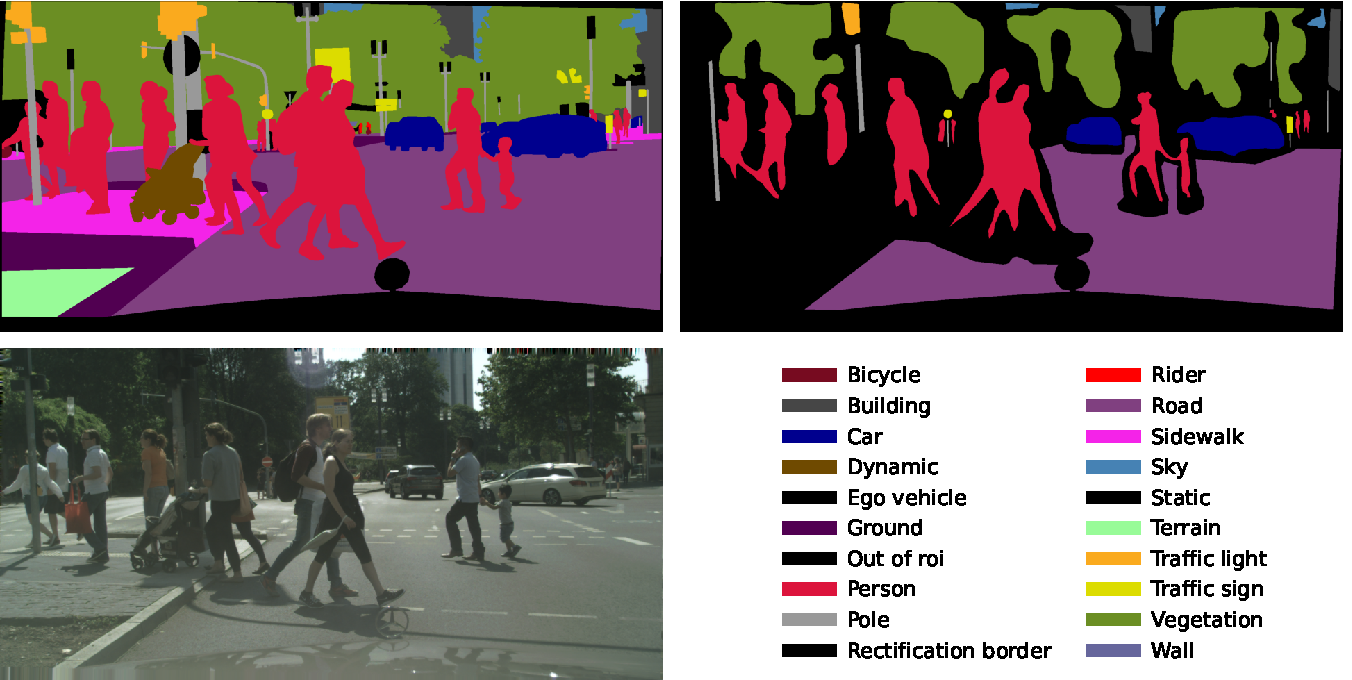
\includegraphics[width=1\columnwidth]{img/2-related-work/1-example-annotation.pdf}
    \caption[Example of semantic segmentation annotations]{Example of an urban scene with semantic segmentation annotations from the Cityscapes Dataset \cite{Cityscapes}. Top-left: Fine-grained ground-truth annotation. Top-right: coarse annotation. Bottom-left: image. Bottom-right: semantic classes.}
    \label{fig:semantic-segmentation-example}
\end{figure}
    

%%%%%% Subsection: architectures


\subsection{Architectures}


Deep convolutional neural networks have emerged as the leading approach to address semantic segmentation \cite{Chai2021}. Unlike other tasks such as classification, where the output of the models is a vector with one score per class, semantic segmentation requires the prediction of a score for each pixel of the input image and its corresponding semantic class, making it a computationally demanding operation. 

Although researchers have proposed successful architectures that process images while maintaining the spatial dimension internally in all layers \cite{Sun2019HighResolutionRF}, the use of such architectures comes with a high computational cost.
For this reason, the most common architectures downsample the images with convolutional layers to reduce computational requirements and upsample the compact representation to produce an output of the same size as the input. This takes advantage of spatial locality, making the process more computationally efficient \cite{SemanticSegmentationSurvey}.


One of the earliest architectures that proposes the aforementioned approach is the Fully Convolutional Network (FCN) \cite{FCN}. FCN uses several convolutional layers to reduce the spatial dimension of the input image while increasing the number of channels to maintain local semantic information. A final pixel-wise layer is used to generate a detailed segmentation, as illustrated in Figure \ref{fig:fcn}.


\begin{figure}
    \centering
    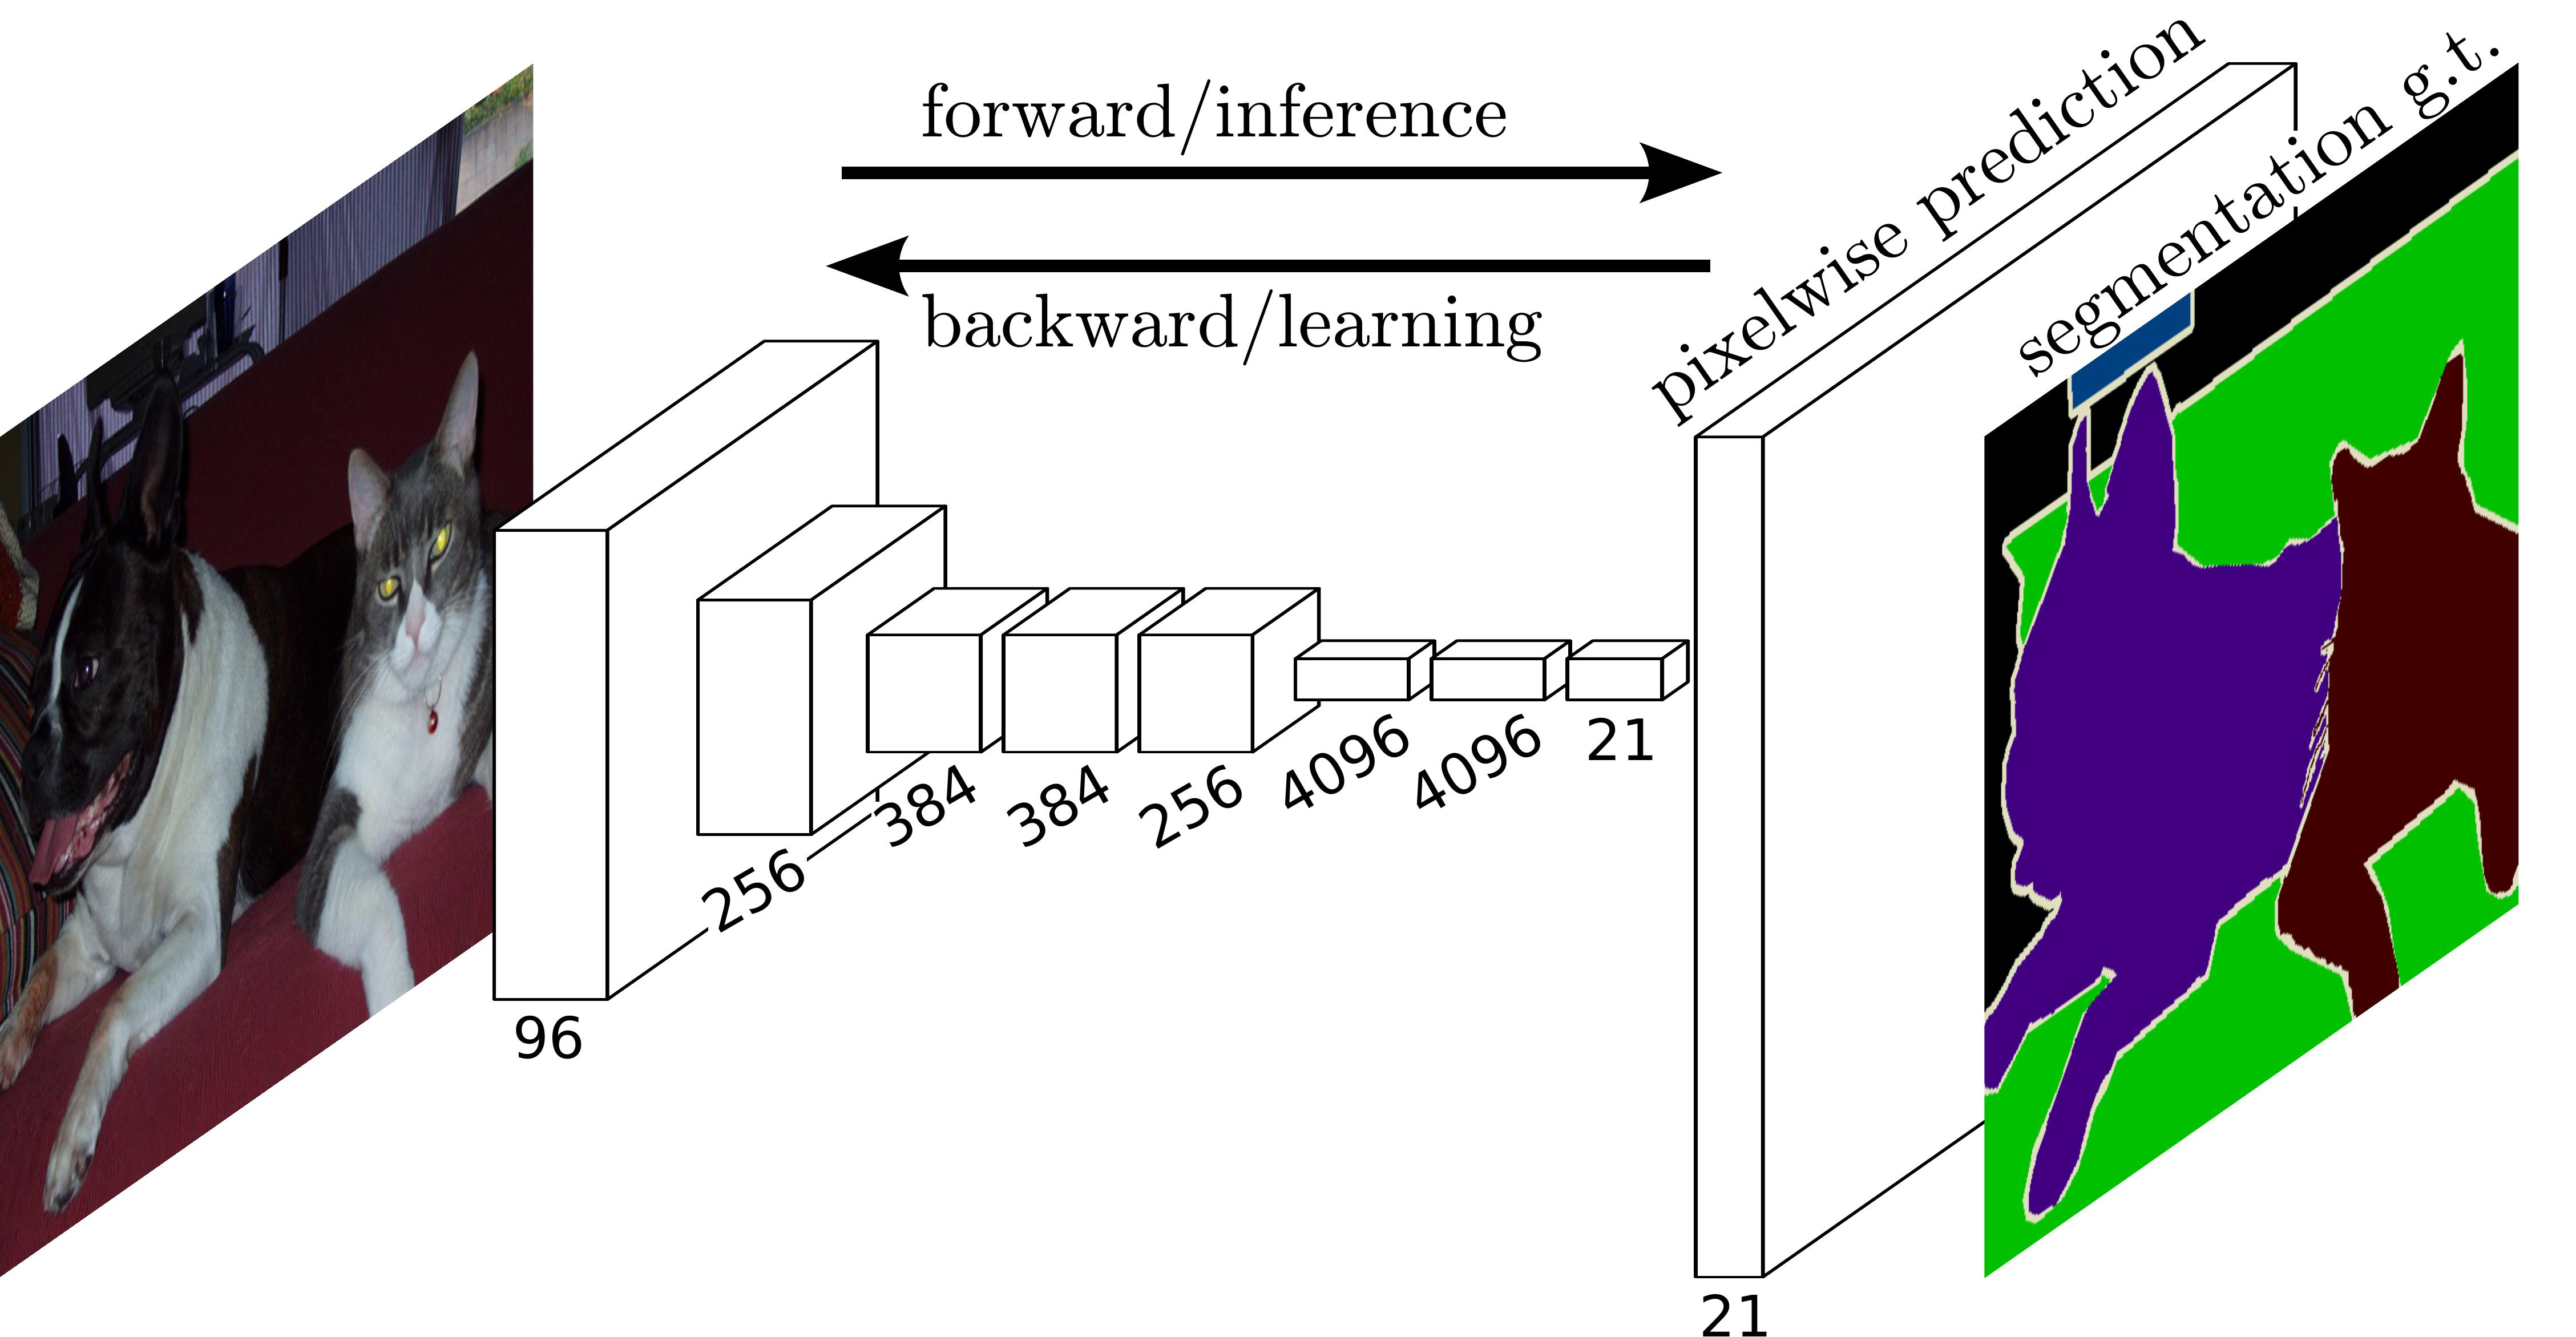
\includegraphics[width=0.7\columnwidth]{img/2-related-work/design-fcn.jpeg}
    \caption[Fully convolutional network n (FCN)]{Fully convolutional network for semantic segmentation \cite{FCN}}
    \label{fig:fcn}
\end{figure}

To prevent the potential loss of spatial information due to the downsampling layers, researchers proposed the U-NET architecture \cite{UNET}, a symmetric encoder-decoder design (shown in Figure \ref{fig:unet}) that incorporates connections between the downsampling and upsampling stages. These connections merge the semantic information from the higher layers with the spatial information from the lower layers obtaining fine-grained predictions.

Many contemporary semantic segmentation architectures are being proposed in this direction, aiming to compactly encode semantic information while minimizing spatial information loss. As an example, two popular approaches are the use of atrous convolutions and multi-resolution features. 
Atrous convolutions \cite{DeeplabV3}, also known as dilated convolutions, increase the receptive field by introducing gaps between kernel elements, resulting in the efficient processing of high-resolution images without increasing the number of parameters. On the other hand, multi-resolution features, used in HRNet \cite{HRNET}, involves using convolutions of different sizes in parallel to extract information at multiple levels of resolution and combine it for a more robust representation. This strategy allows the use of features with complementary information, improving accuracy and enabling fine-grained predictions. 

Since these models are complex and require large amounts of data, training strategies such as curriculum learning \cite{Zhang2017}, knowledge distillation \cite{Tung2019SimilarityPreservingKD}, and adversarial losses \cite{Tsai_adaptseg_2018} are commonly used to improve their performance. For this reason, much of the research efforts are based on exploring new training strategies and creating datasets with increased variability, particularly in domains such as urban scenes. In the following subsection, we introduce some of the most widely used datasets and benchmarks for training and compare the performance of these models.

\begin{figure}
    \centering
    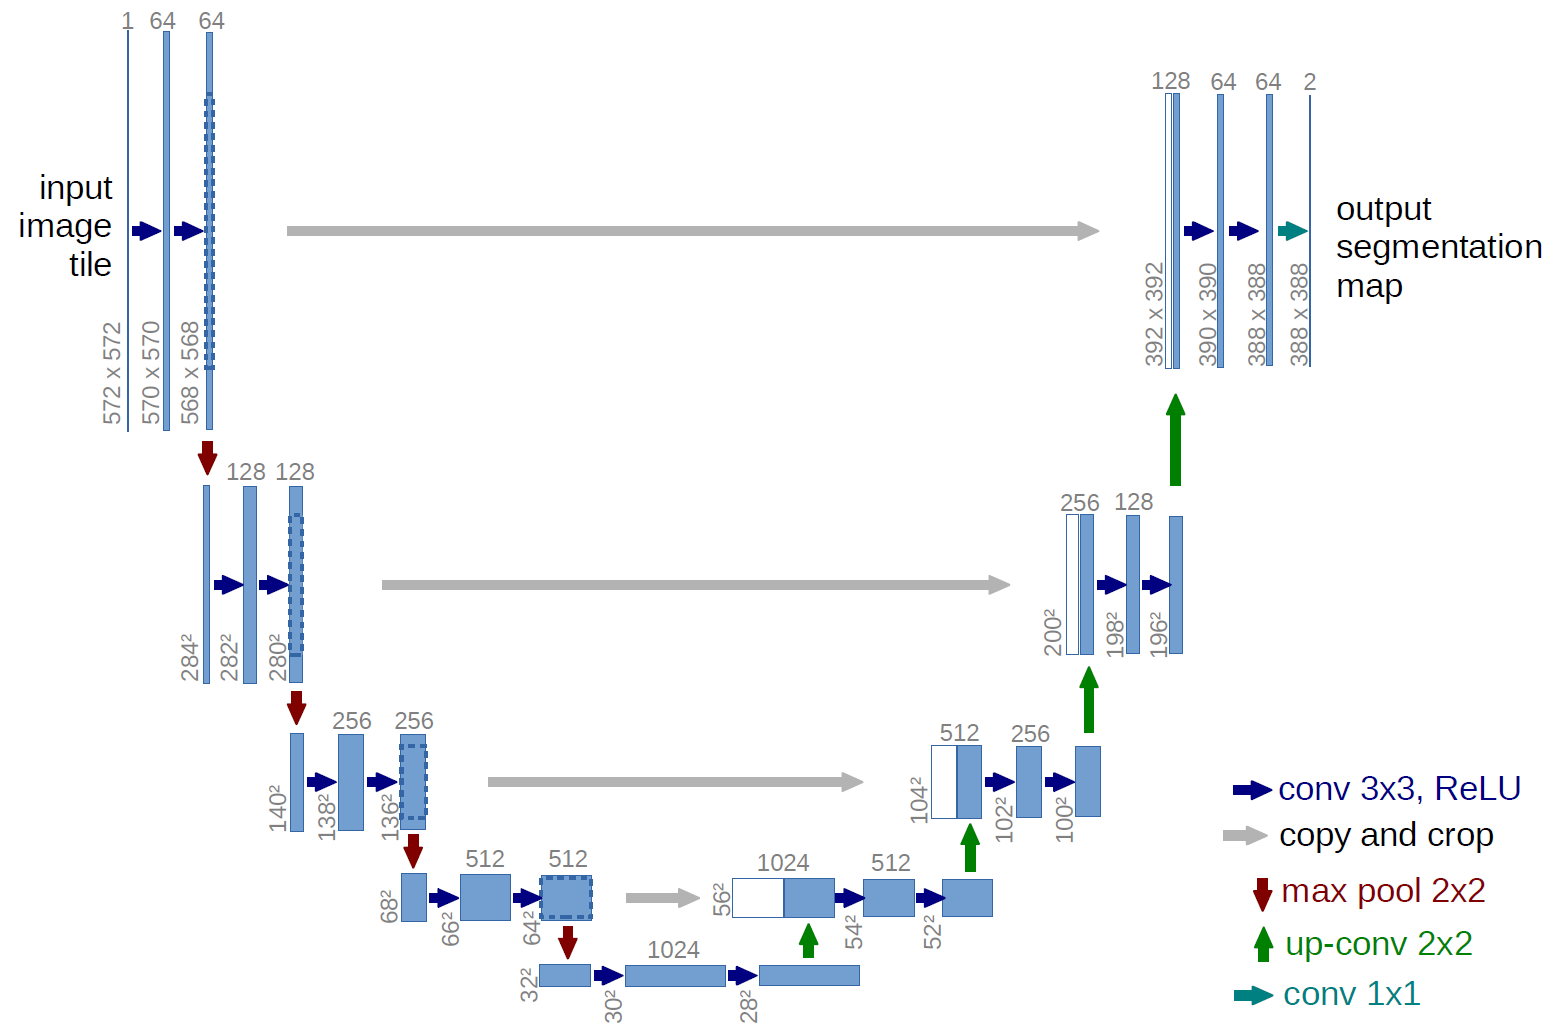
\includegraphics[width=0.75\columnwidth]{img/2-related-work/u-net-architecture.png}
    \caption[U-NET architecture]{U-NET architecture. Source \cite{UNET}.}
    \label{fig:unet}
\end{figure}

\subsection{Datasets and benchmarks}

%% Example of real datasets
\begin{figure}
\centering
  \begin{subfigure}[b]{0.49\columnwidth}
    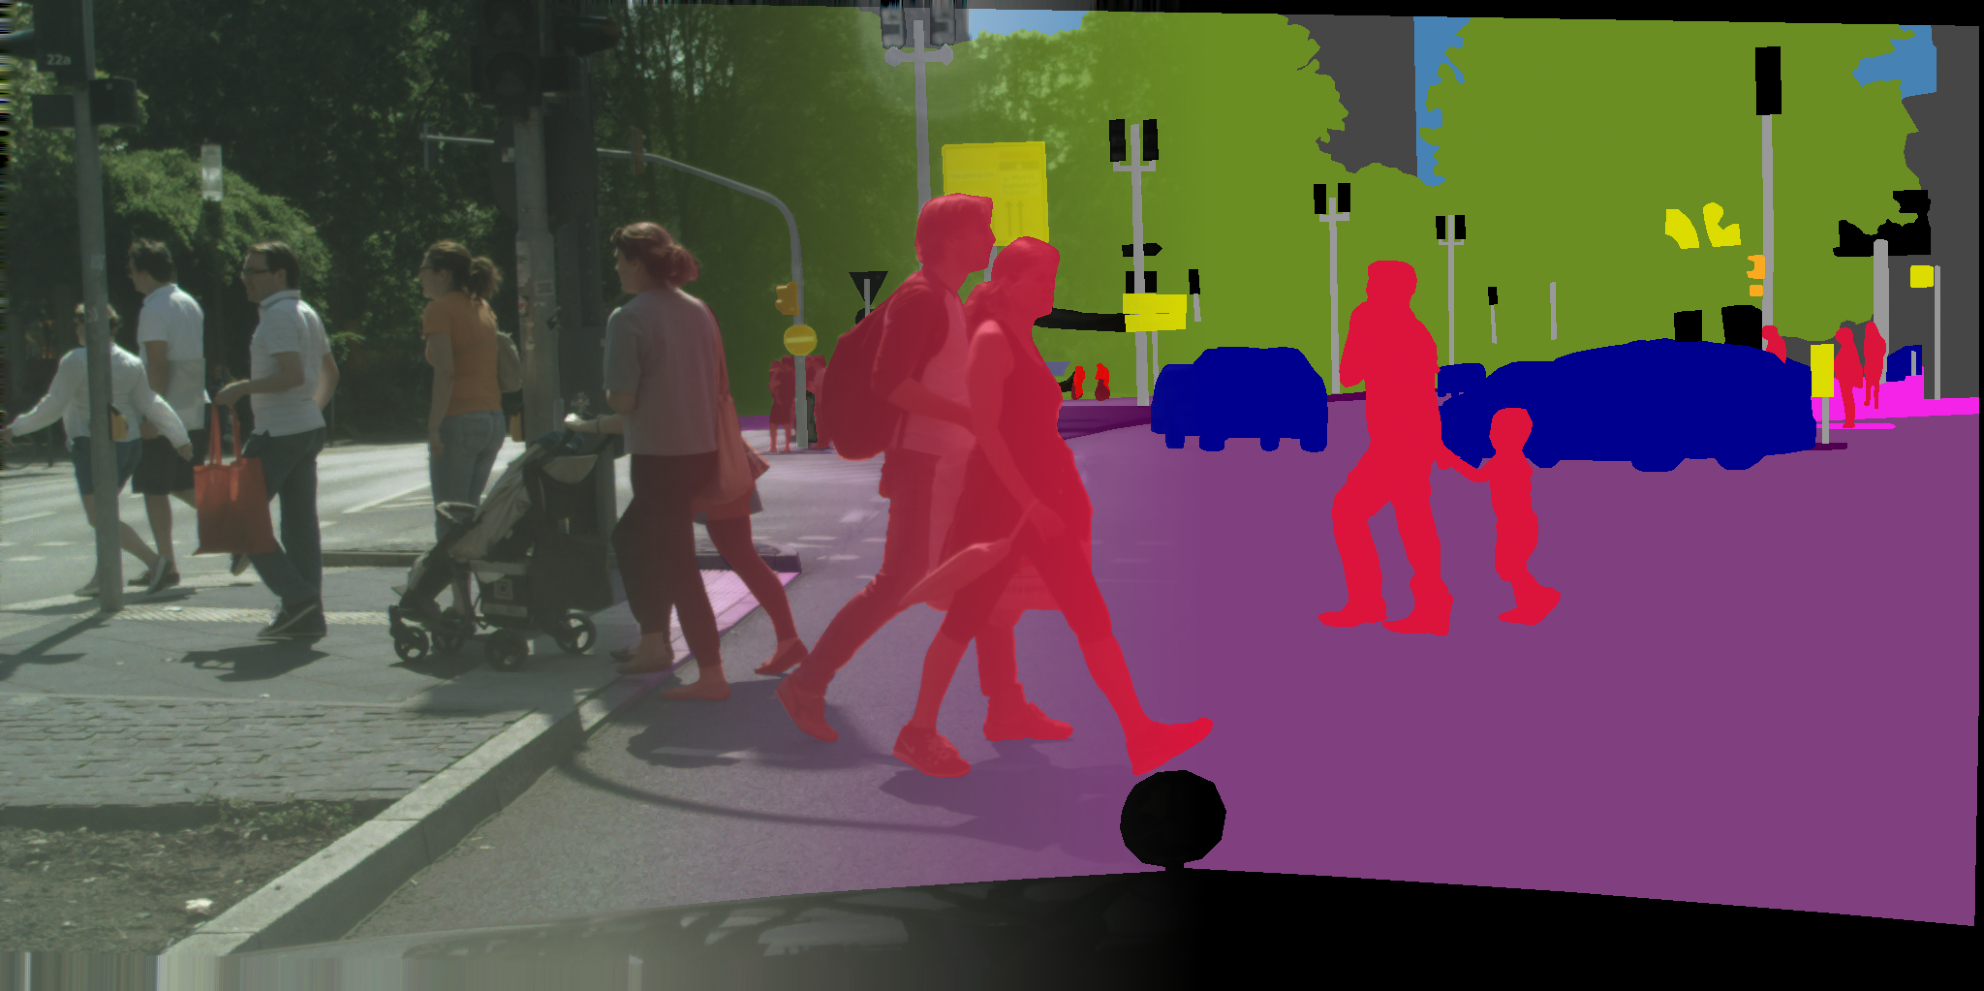
\includegraphics[width=\columnwidth]{img/2-related-work/cityscapes_semantic_segmentation_overlay.png}
    \caption{Cityscapes \cite{Cityscapes}}
    \label{fig:example-city}
  \end{subfigure}
  %
  \begin{subfigure}[b]{0.49\columnwidth}
    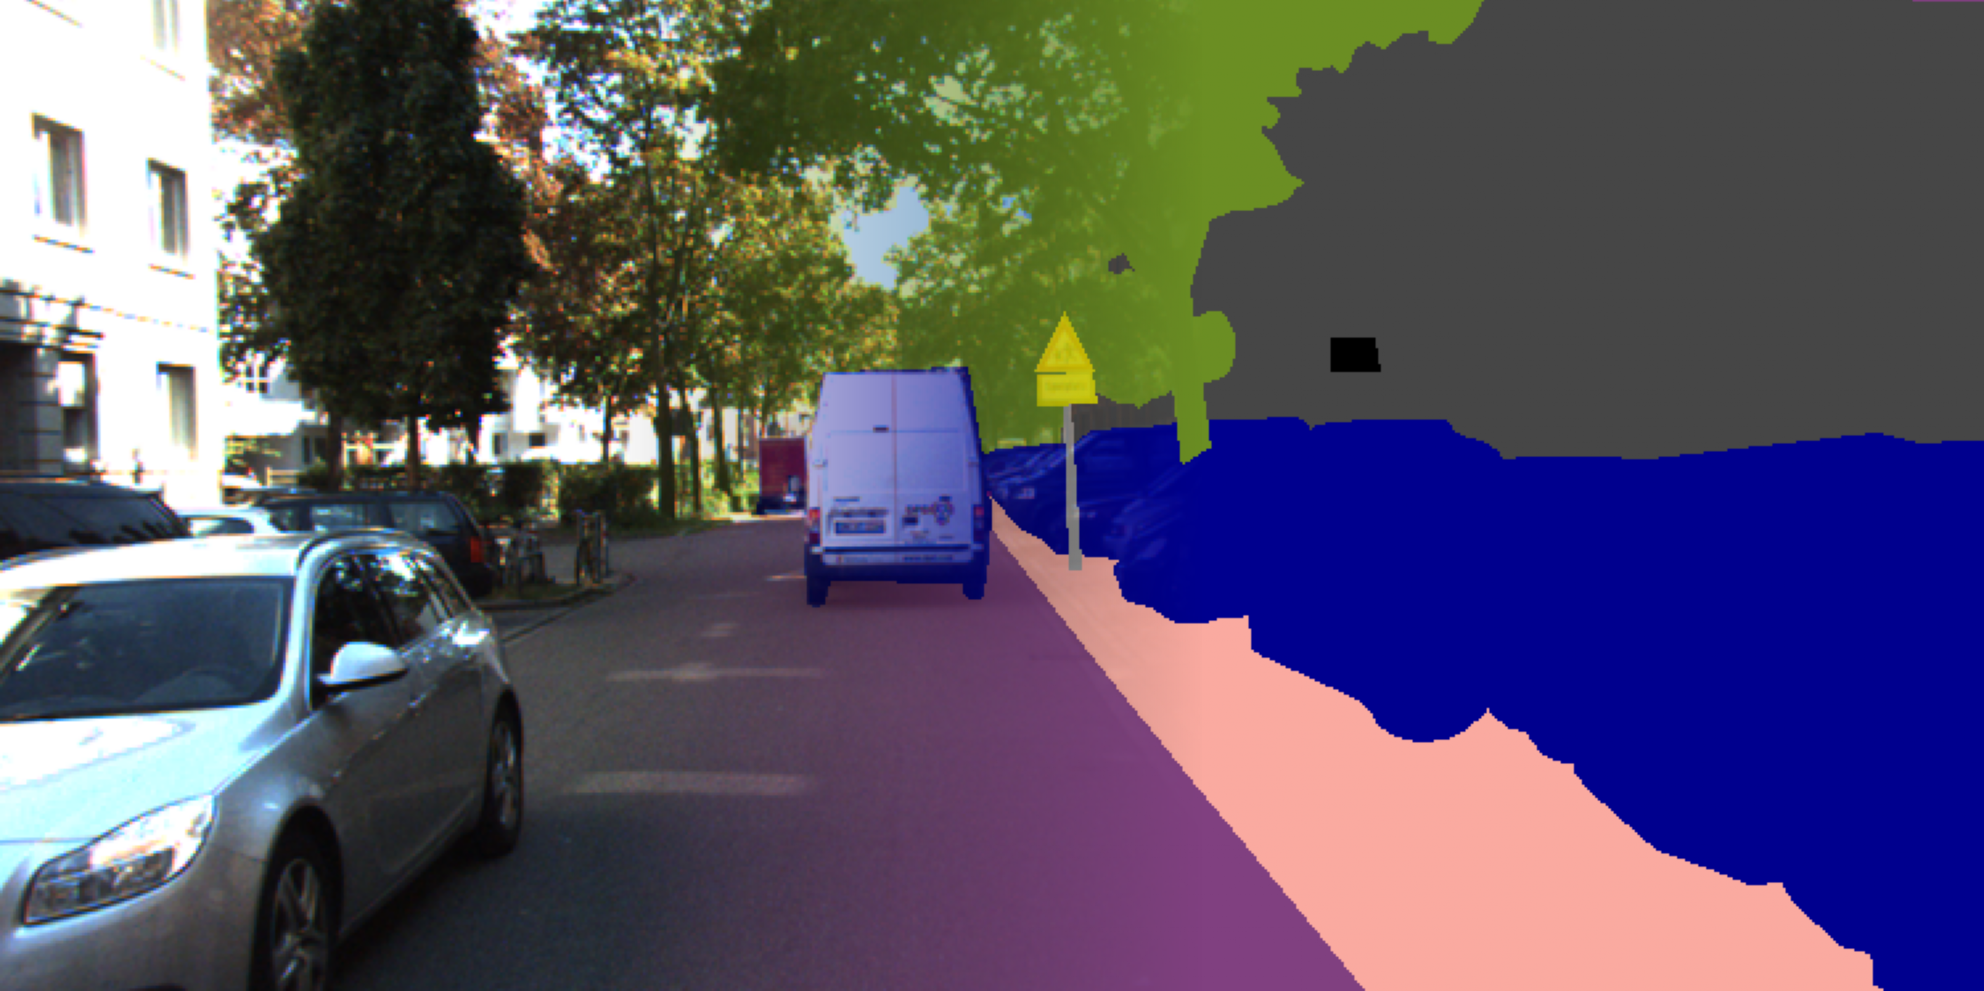
\includegraphics[width=\columnwidth]{img/2-related-work/kitti_semantic_segmentation_overlay.png}
    \caption{KITTI \cite{kitty}}
    \label{fig:example-kitti}
  \end{subfigure}

  \begin{subfigure}{0.49\columnwidth}
    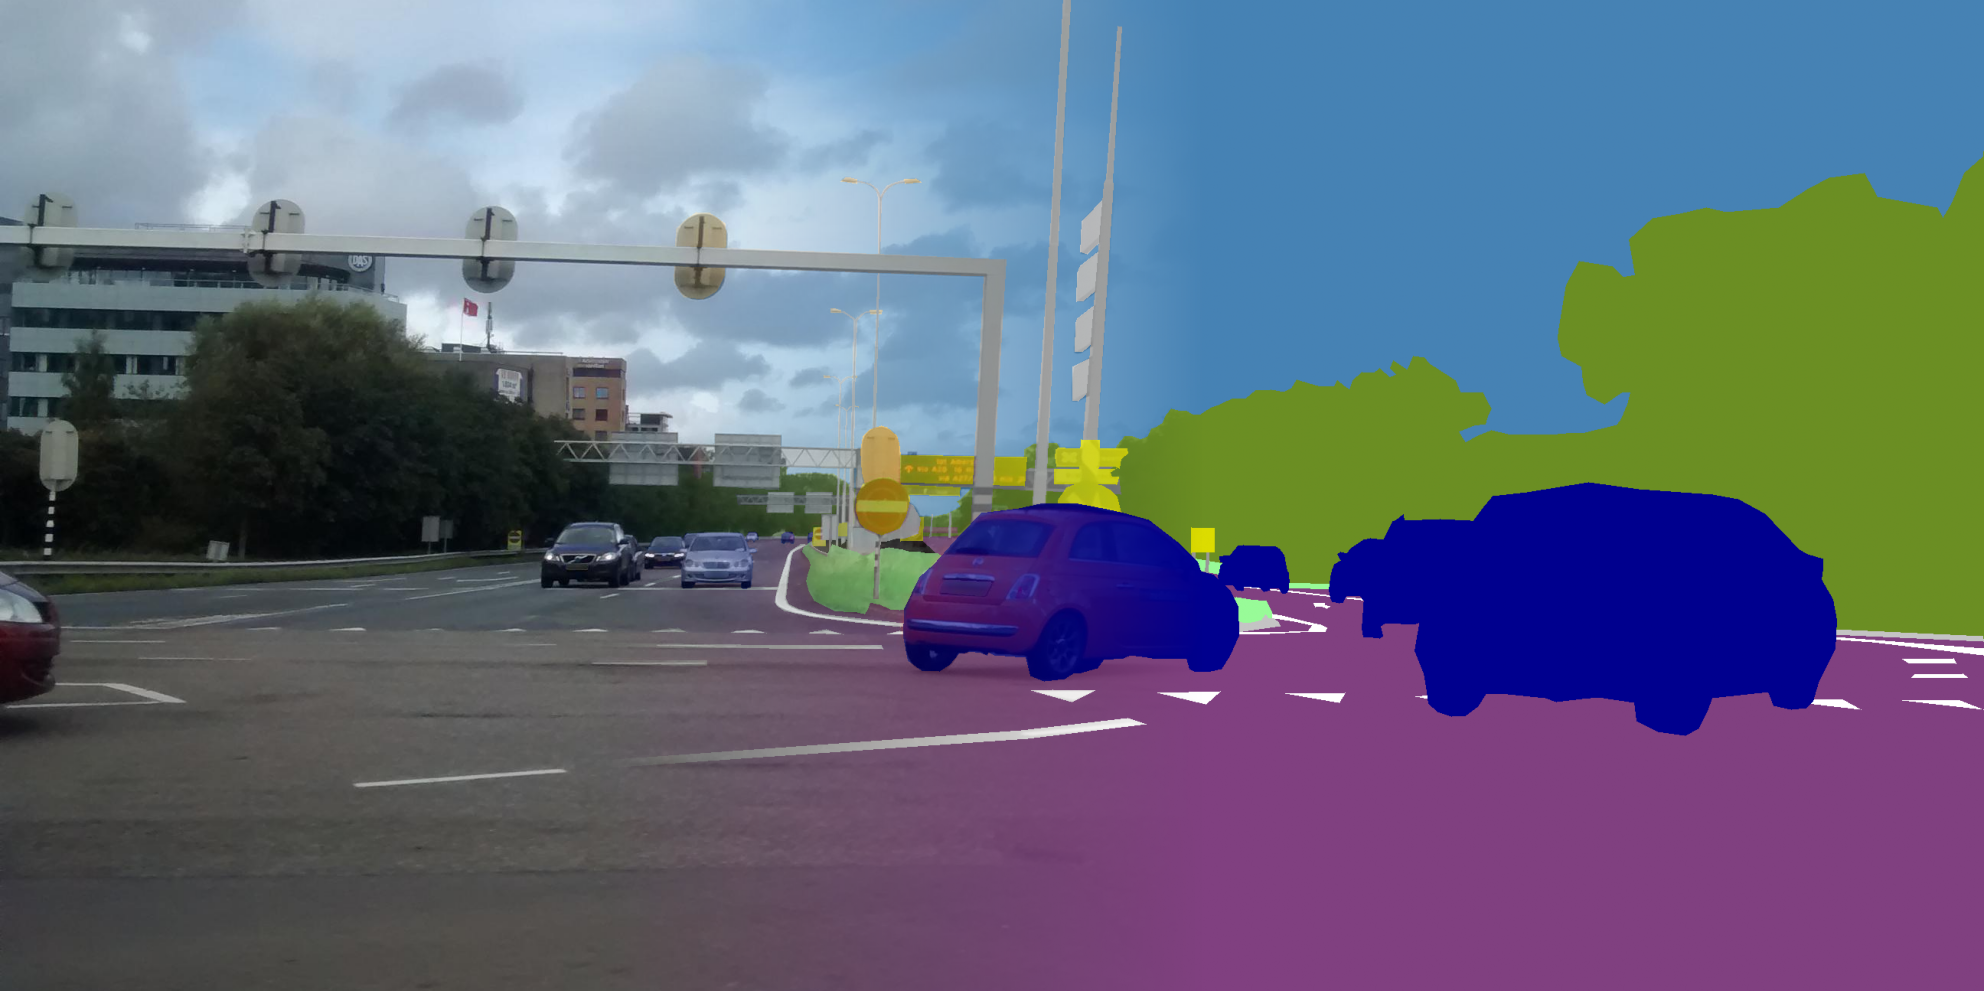
\includegraphics[width=\columnwidth]{img/2-related-work/mapilliary_semantic_segmentation_overlay.png}
    \caption{Mapillary Vistas \cite{mapilliary}}
    \label{fig:example-dbb100k}
  \end{subfigure}
  %
  \begin{subfigure}[b]{0.49\columnwidth}
    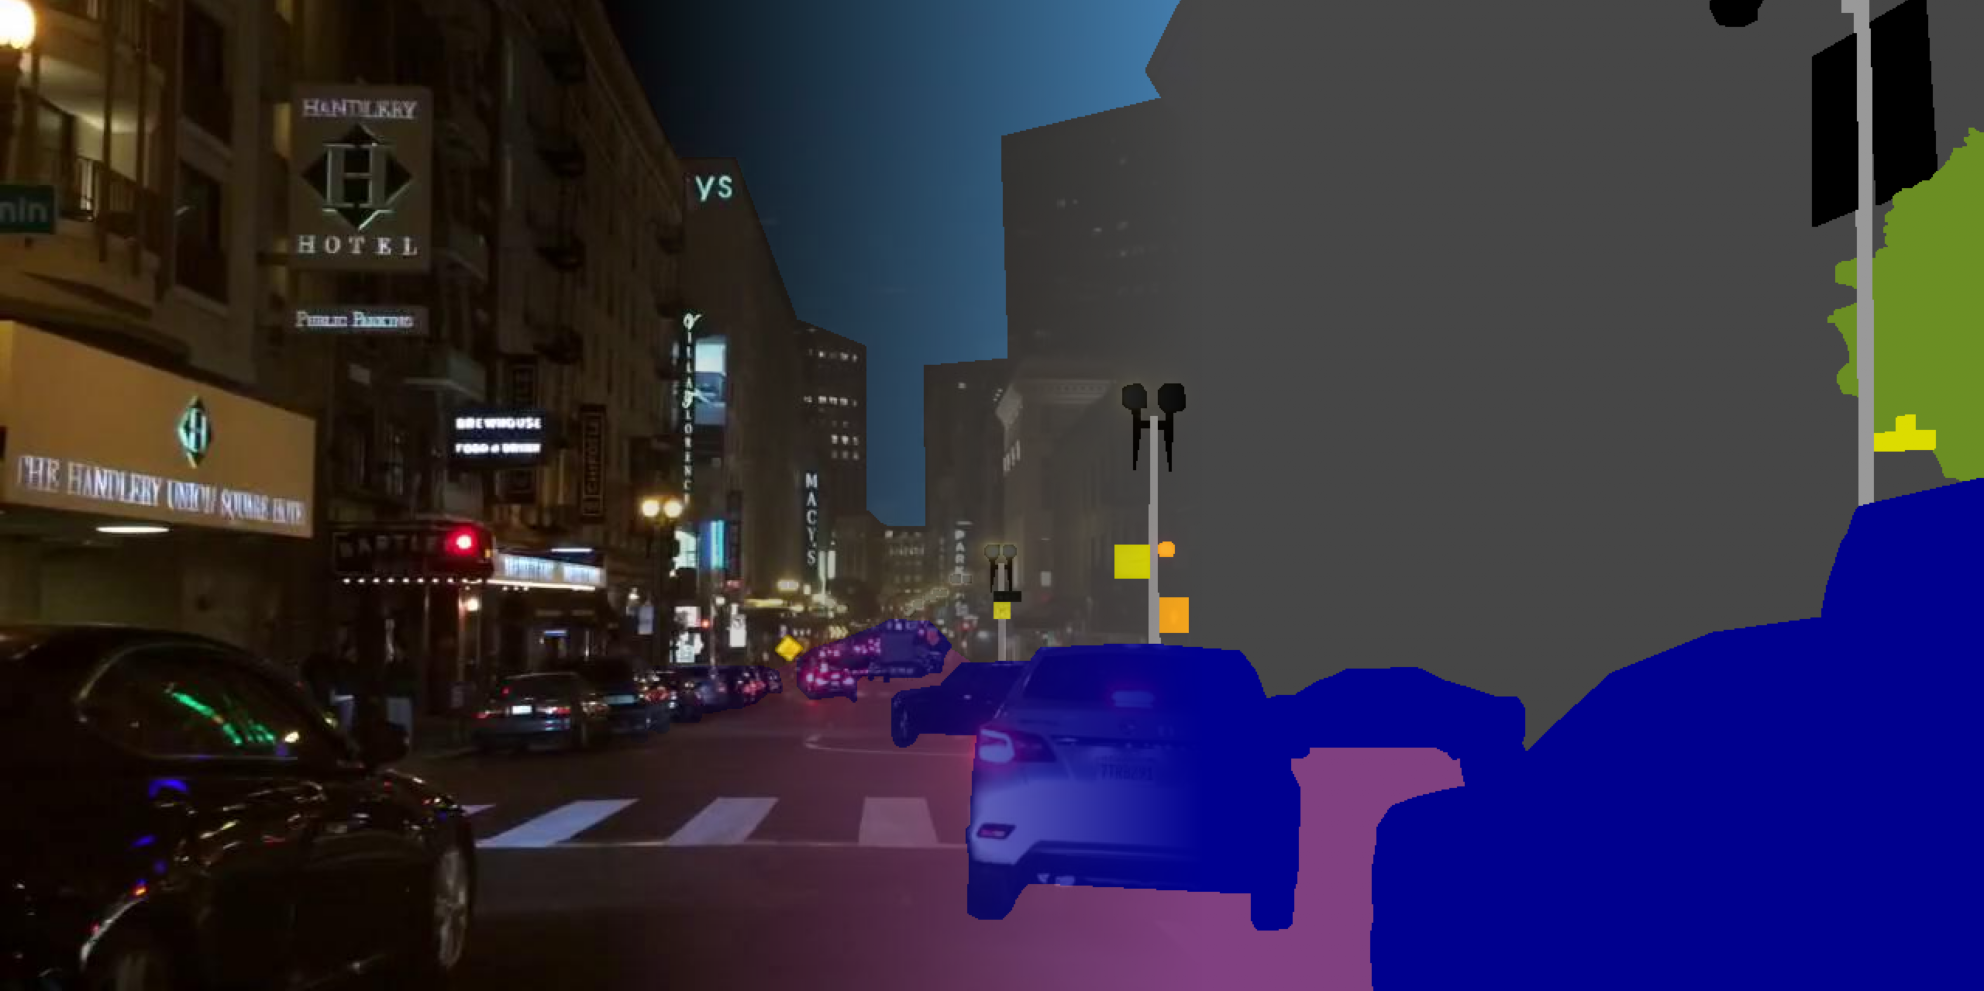
\includegraphics[width=\columnwidth]{img/2-related-work/dbb100k_semantic_segmentation_overlay.png}
    \caption{Berkeley Deepdrive Dataset \cite{BDD100K}}
    \label{fig:example-mapilliary}
  \end{subfigure}

  \caption[Visual examples of real datasets for urban scenes]{Visual examples of real datasets for urban scenes}
    \label{fig:real-datasets-examples}

\end{figure}

%Semantic segmentation is a challenging task that requires complex deep learning models, massive amounts of data, and specialized training strategies to achieve competitive performances. 
One of the main factors contributing to the success of semantic segmentation models is the availability of large datasets with high-quality annotations for training and evaluation. To address this issue, the research community has created several public datasets and benchmarks to train these models and unify comparisons. In this section, we review the most commonly used real datasets for semantic segmentation of urban scenes. 

Urban scenes datasets are composed of images taken from cameras on moving vehicles or captured by drones, and commonly they show the urban environment from the driver's point of view. These images are annotated with pixel-level labels with different semantic categories, such as roads, buildings, pedestrians, and vehicles. The annotations are used as ground truth segmentation maps to train and evaluate semantic segmentation models. Some of the most widely used datasets in this area, illustrated in Figure \ref{fig:real-datasets-examples}, are Cityscapes \cite{Cityscapes}, KITTI \cite{kitty}, Mapillary \cite{mapilliary}, and BDD100K \cite{BDD100K}.

Cityscapes \cite{Cityscapes} contains high-quality images of street scenes from 50 different cities across Europe, with pixel-level annotations of 30 different semantic classes. KITTI \cite{kitty} contains images of urban scenes captured by a camera mounted on a moving vehicle and annotated with semantic labels. Mapillary \cite{mapilliary} is a crowd-sourced dataset that contains images taken from street-level perspectives by a large community of users with global coverage. BDD100K \cite{BDD100K} contains diverse and challenging images with different weather conditions in urban and suburban areas. Table \ref{tab:real-datasets} contains information of these and other of the most widely used datasets of urban scenes.

\begin{table}
    \centering
    \begin{tabular}{|c|c|c|c|}
         \hline 
         Dataset & Geographic coverage & Classes & Public images \\
         \hline 
          Cityscapes \cite{Cityscapes} & 50 cities (Germany) & 30 & 
          5,000 (+20,000)  \\ 
          KITTI \cite{kitty}  & 1 city (Germany) & 30 & 200 \\
          Mapillary Vistas \cite{mapilliary}  & Global coverage & 124 & 20,000 \\
          Berkeley DeepDrive \cite{BDD100K}  & 4 cities (USA) & 40 & 10,000 \\
          Wilddash2 \cite{wildash2}  & Global coverage & 30 & 4,256 \\
          Apollo Scape \cite{wang2019apolloscape}  & 4 regions in China & 25  & 146,997 \\
          India Driving Dataset \cite{Varma_2019} & 182 scenes (India)  & 34 & 10,000 \\
          Audi A2D2 \cite{Geyer2020A2D2AA}  & South of Germany & 38 & 41,277 \\
           \hline
    \end{tabular}
    \caption[Summary of widely used real datasets]{Summary of widely used datasets in semantic segmentation of urban scenes}
    \label{tab:real-datasets}
\end{table}

As a way to increase the variability and the number of annotated images, some datasets provide low-quality annotations that can be used for pre-training. For example, Cityscapes provides 20,000 extra coarse annotations (as shown in Figure \ref{fig:semantic-segmentation-example}). However, due to the high cost of manually annotating images with high detail \cite{Lin_2019_ICCV}, these datasets consist of only a few thousand images. Despite the effort to create more diverse and high-quality datasets, a still unsolved problem is the high bias between them. Models trained on a dataset do not generalize correctly to other ones due to differences in image quality, lighting conditions, and annotation criteria \cite{mapilliary}. This issue is known as domain shift and is one of the main challenges in semantic segmentation research.

To enable the comparison of different models under the same conditions, it is necessary to define a set of evaluation metrics. To address this problem, the research community has created benchmarks associated with each of the main datasets to evaluate models under the same conditions. The most common metric for semantic segmentation is Intersection over Union (IoU), which measures the overlap between the predicted and ground truth segmentation maps. Although other metrics, such as precision and recall, are also used to evaluate model performance, and the choice of new metrics is still an open discussion in the research community \cite{metrics1, Zhang2021RethinkingSS, Cho2021WeightedIO}.




\subsection{Synthetic data}




%\begin{table}
%    \centering
%    \begin{tabular}{|c|c|c|c|}
%         \hline 
%         Dataset & Year & Engine & Notes \\
%         \hline 
%          TORCS & - & - & - \\
%          Virtual KITTI \cite{kitty} & - & - & - \\
%          GTAVision \cite{gtav} & - & - & - \\
%          SYNTHIA \cite{SYNTHIA} & - & - & - \\
%          VIPER & - & - & - \\
%          CARLA \cite{CarlaSimulator} & - & - & - \\
%          AADS & - & - & - \\
%          PreSIL & - & - & - \\
%          MSS & - & - & - \\
%           \hline
%    \end{tabular}
%    \caption[Summary common used synthetic datasets]{Summary of widely used synthetic datasets in semantic segmentation. \emph{NOTA. Citar a Rober, MTAP.}}
%    \label{tab:synthetic-datasets}
%\end{table}


Since the first attempts to develop autonomous driving systems, a major challenge has been the availability of datasets that can capture the variability of driving environments \cite{pomerleau:alvinn}. To address this issue, researchers have employed synthetic data generated by simulators to increase this variability.

In recent years, simulators based on game engines, such as Unity \cite{kitty, SYNTHIA} or GTA V \cite{gtav}, have become popular. Simulators allow the extraction of complete information from the environment, including semantic classes, 3D boxes, multiple perspectives, or depth maps in a pixel-accurate way, as in the examples illustrated in Figure \ref{fig:synthetic-datasets-examples}. 
%Table \ref{tab:synthetic-datasets} provides an overview of widely used synthetic datasets in autonomous driving research.
Other techniques, such as the use of Generative Adversarial Networks \cite{NIPS2014_5ca3e9b1}, have also been employed to increase the amount of data and variability from pre-existing datasets. These methods are typically employed to alter weather or light conditions of scenes, or even to introduce new elements into images.

However, training or pre-training on synthetic data presents challenges due to domain adaptation problems. The domain adaptation problems arise because of the difference in image distributions between synthetic data used for training models and real-world images. Due to this difference, systems lose efficiency when deployed in real-life situations. To mitigate this issue, two primary strategies are used: input and output adaptation.

Input adaptation involves adjusting the synthetic images used during the training step to make them more photorealistic. This can be achieved by using increasingly realistic simulators or by employing generative models to adapt the style of simulator images to make them more photorealistic. However, there is no general consensus on whether photorealism is a necessary aspect that can be solved by increasing the variability in the datasets.

Output adaptation involves incorporating strategies during the training of semantic segmentation models to increase their generalization and reduce the impact of the difference between synthetic and real distributions. This group of strategies includes the use of transfer learning, curriculum learning \cite{Zhang2017}, knowledge distillation \cite{Tung2019SimilarityPreservingKD}, or adversarial losses \cite{Tsai_adaptseg_2018}.

In conclusion, the generation of scenarios capable of including as much variability as possible is fundamental for the development of semantic segmentation systems. Synthetic datasets can include environmental situations that are difficult to simulate and can reduce the need for large real-world datasets, which is crucial for the development of more robust autonomous driving systems. For these reasons, both the scientific community and the industry are putting great efforts into developing new methods for the creation of synthetic data and techniques to reduce the problems of domain shift and domain adaptation.


%% Example of real datasets
\begin{figure}
\centering
  \begin{subfigure}[b]{0.49\columnwidth}
    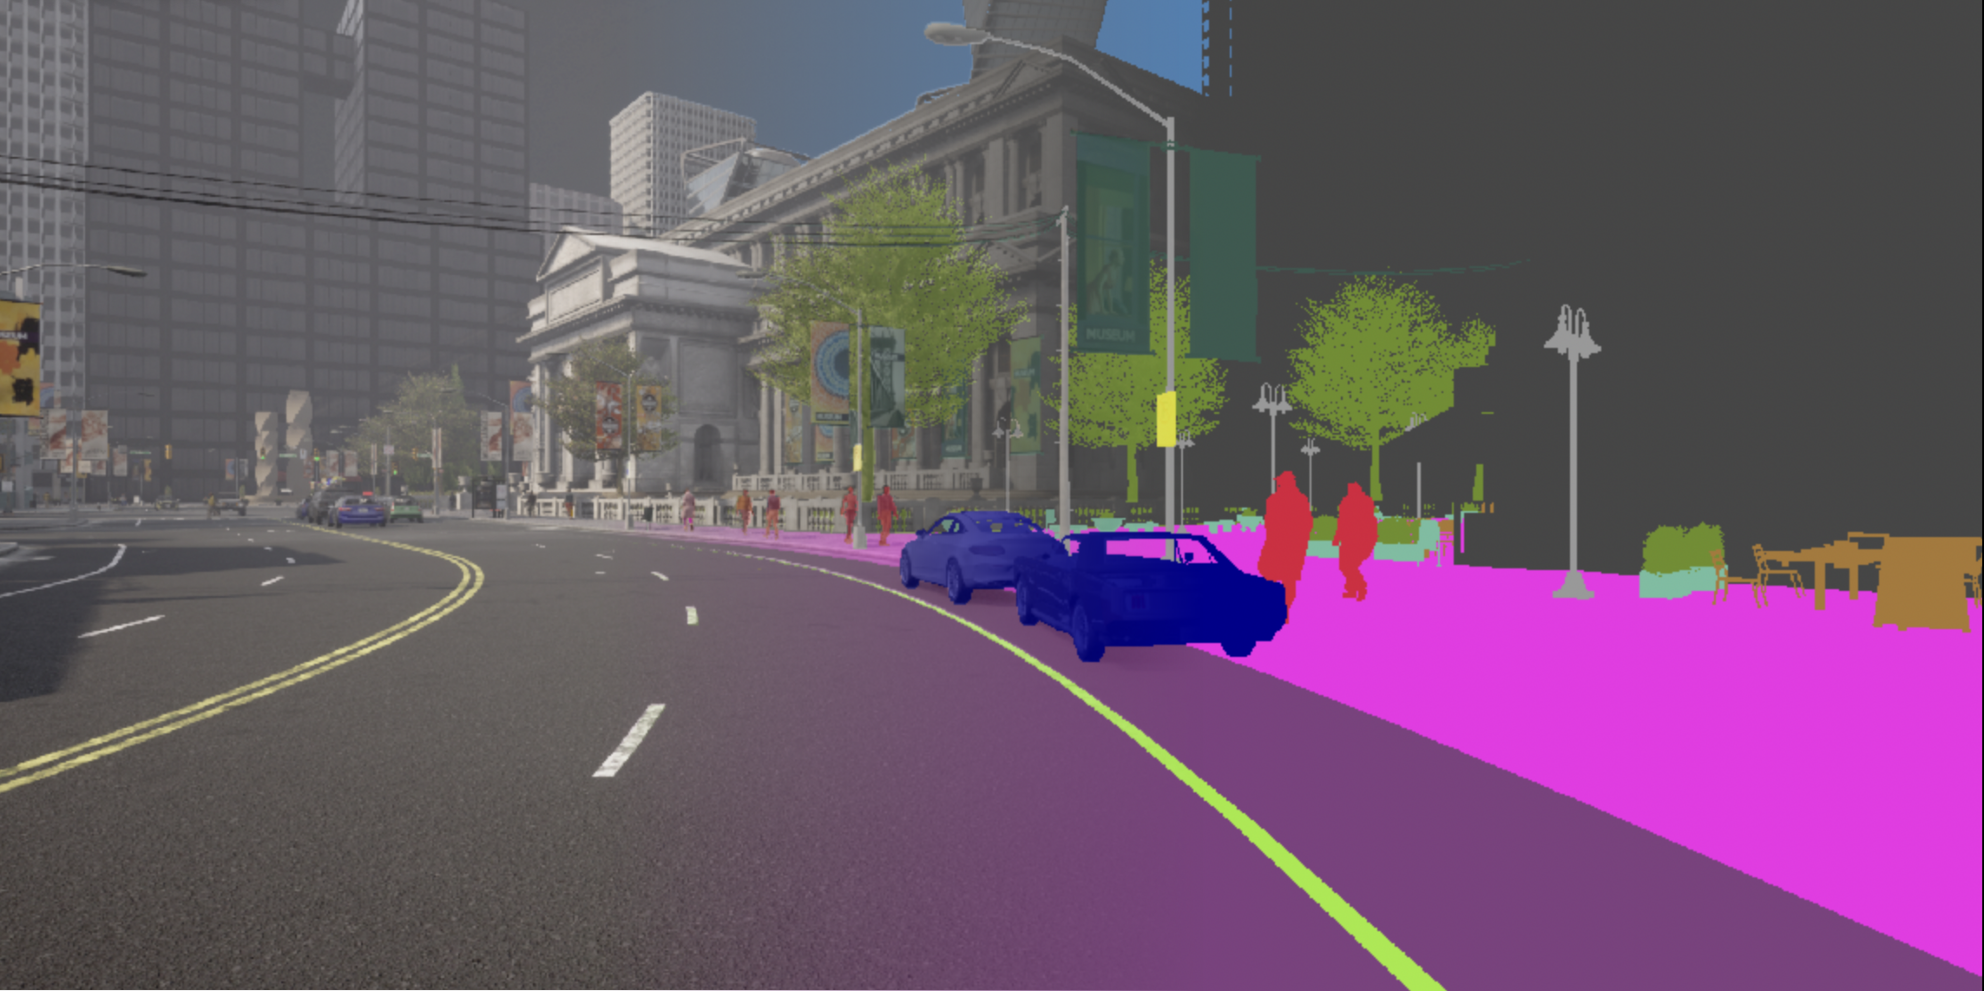
\includegraphics[width=\columnwidth]{img/2-related-work/carla_semantic_segmentation_overlay.png}
    \caption{Carla Simulator \cite{CarlaSimulator}}
    \label{fig:example-carla}
  \end{subfigure}
  %
  \begin{subfigure}[b]{0.49\columnwidth}
    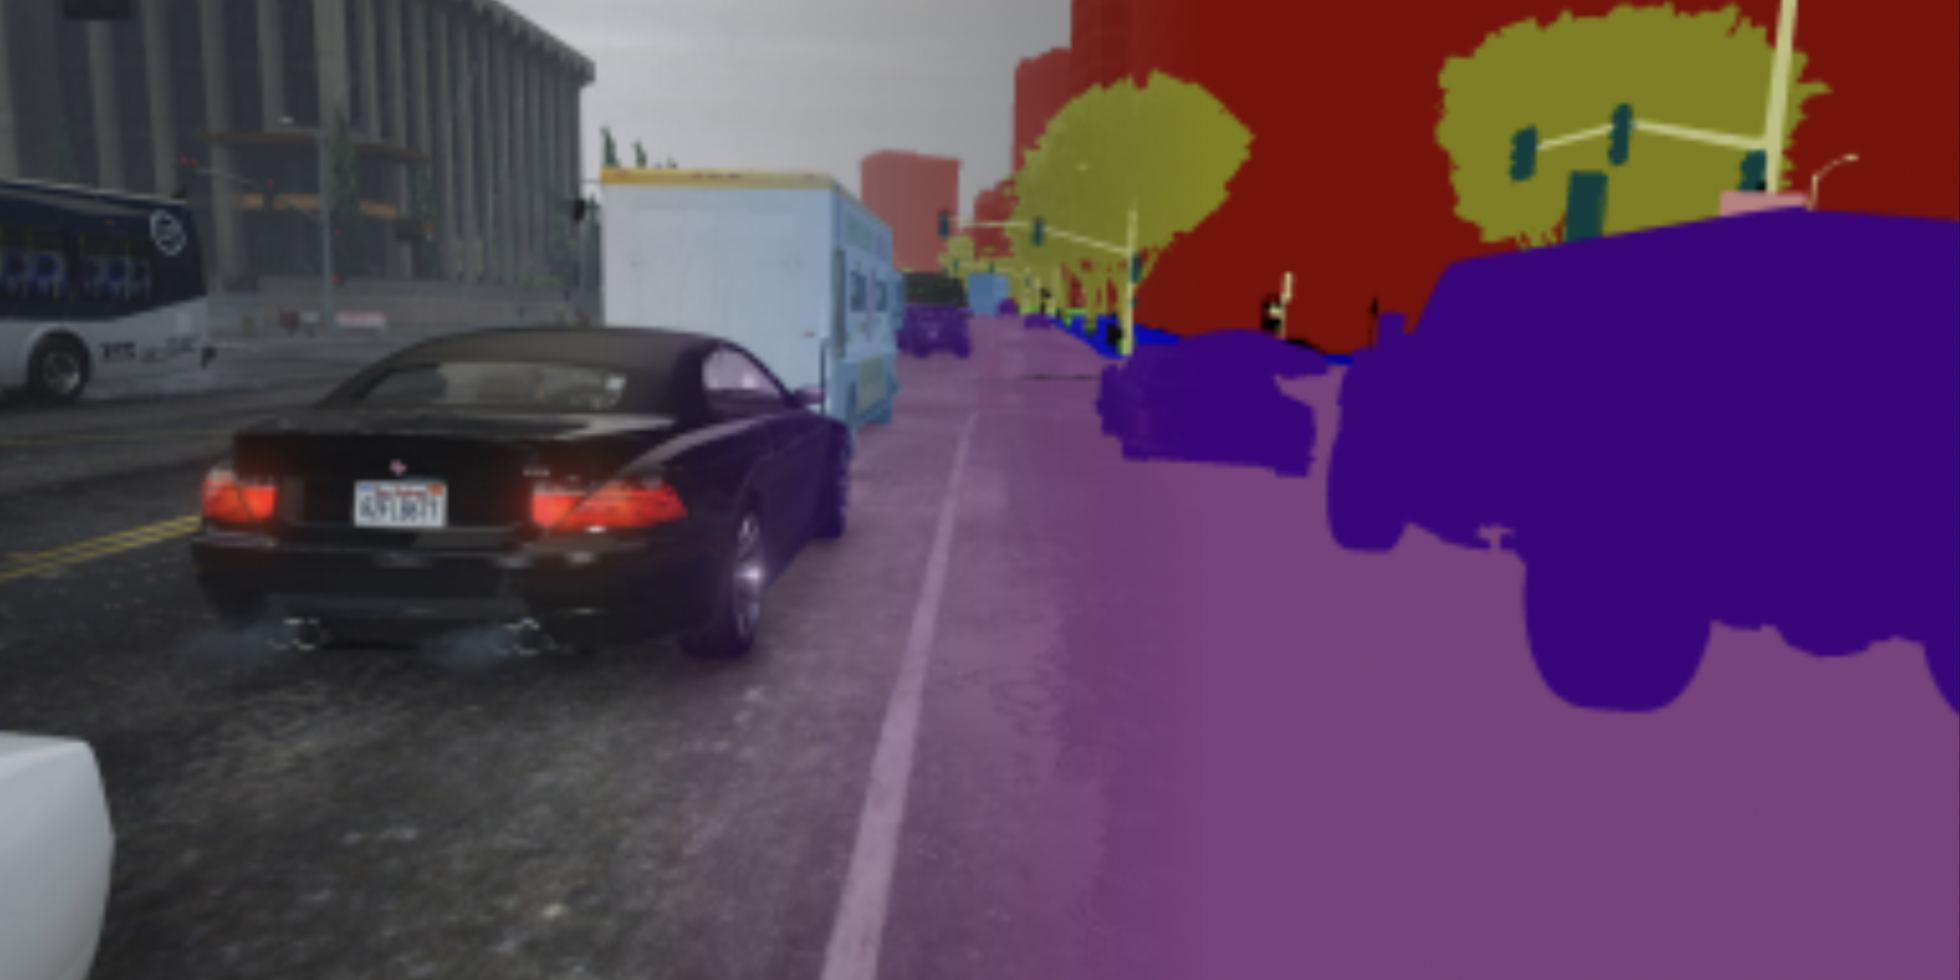
\includegraphics[width=\columnwidth]{img/2-related-work/gtav_semantic_segmentation_overlay_resized.png}
    \caption{GTA Vision \cite{gtav}}
    \label{fig:example-gta}
  \end{subfigure}

  \begin{subfigure}{0.49\columnwidth}
    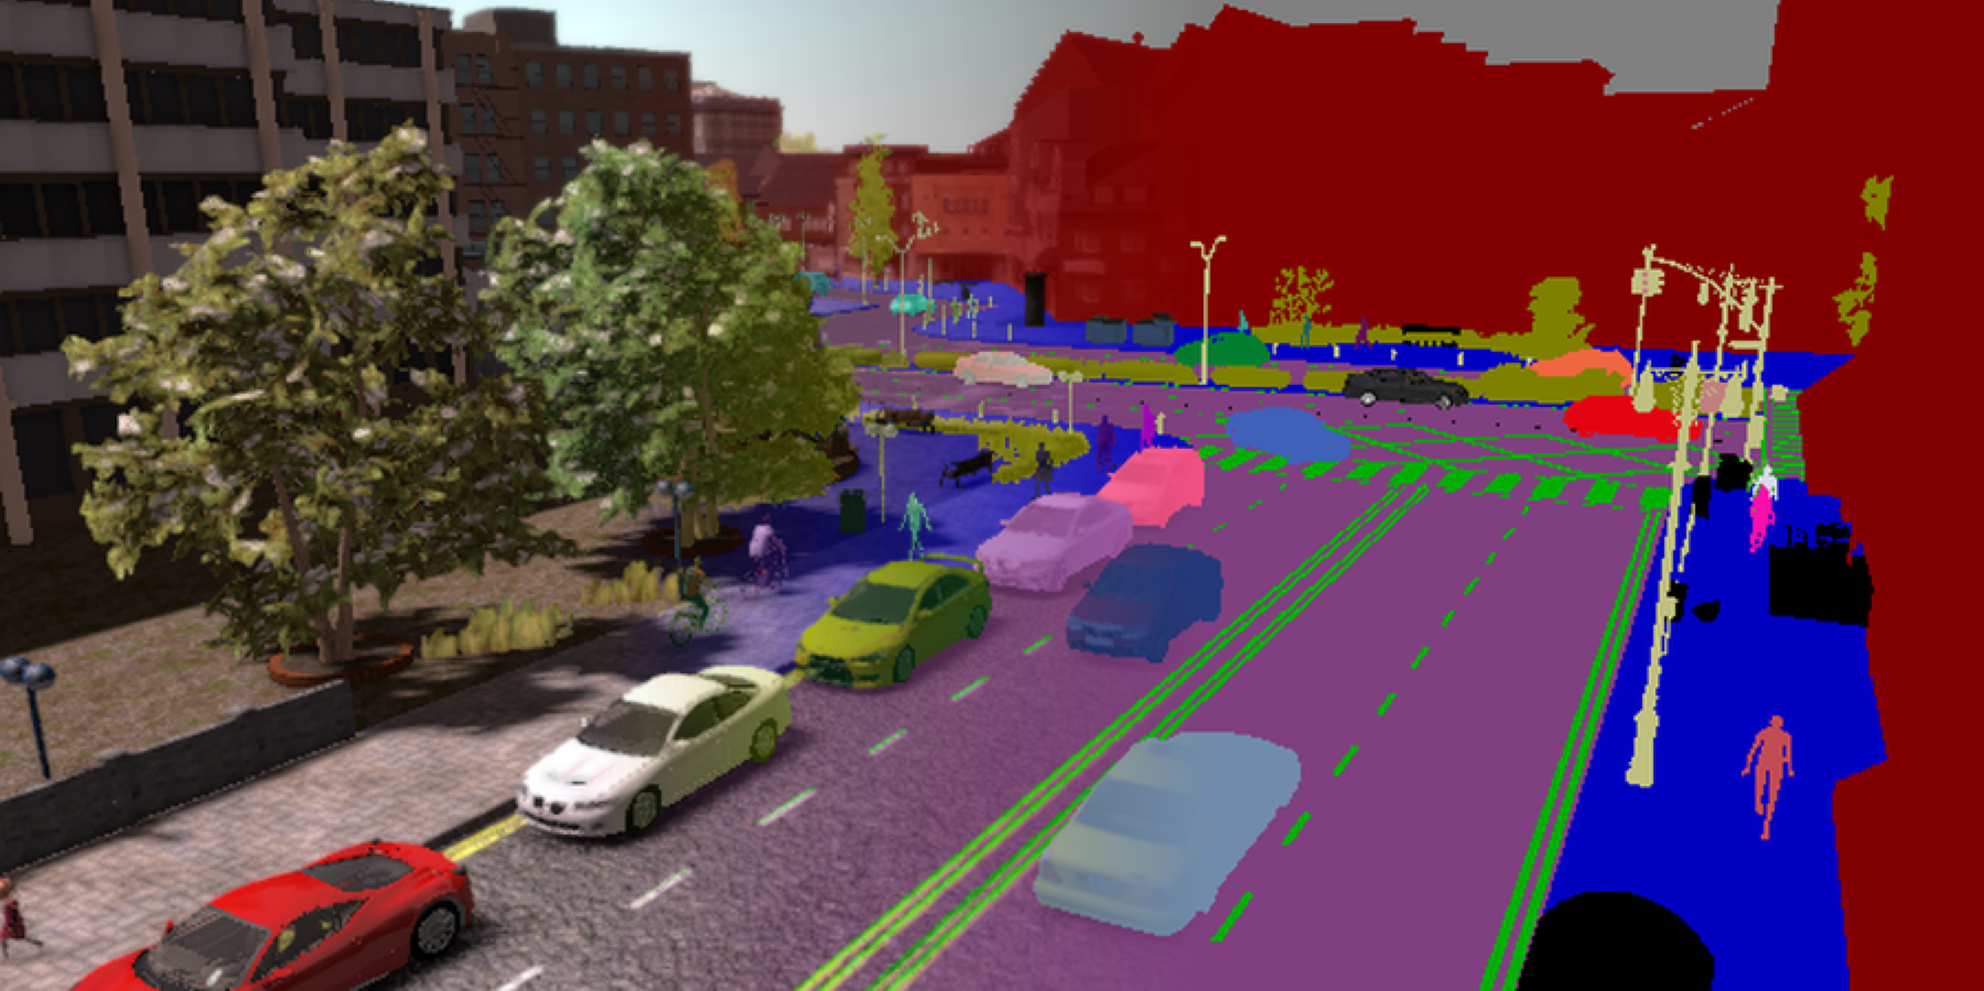
\includegraphics[width=\columnwidth]{img/2-related-work/syntia_semantic_segmentation_overlay.png}
    \caption{SYNTHIA \cite{SYNTHIA}}
    \label{fig:example-syntia}
  \end{subfigure}
  %
  \begin{subfigure}[b]{0.49\columnwidth}
    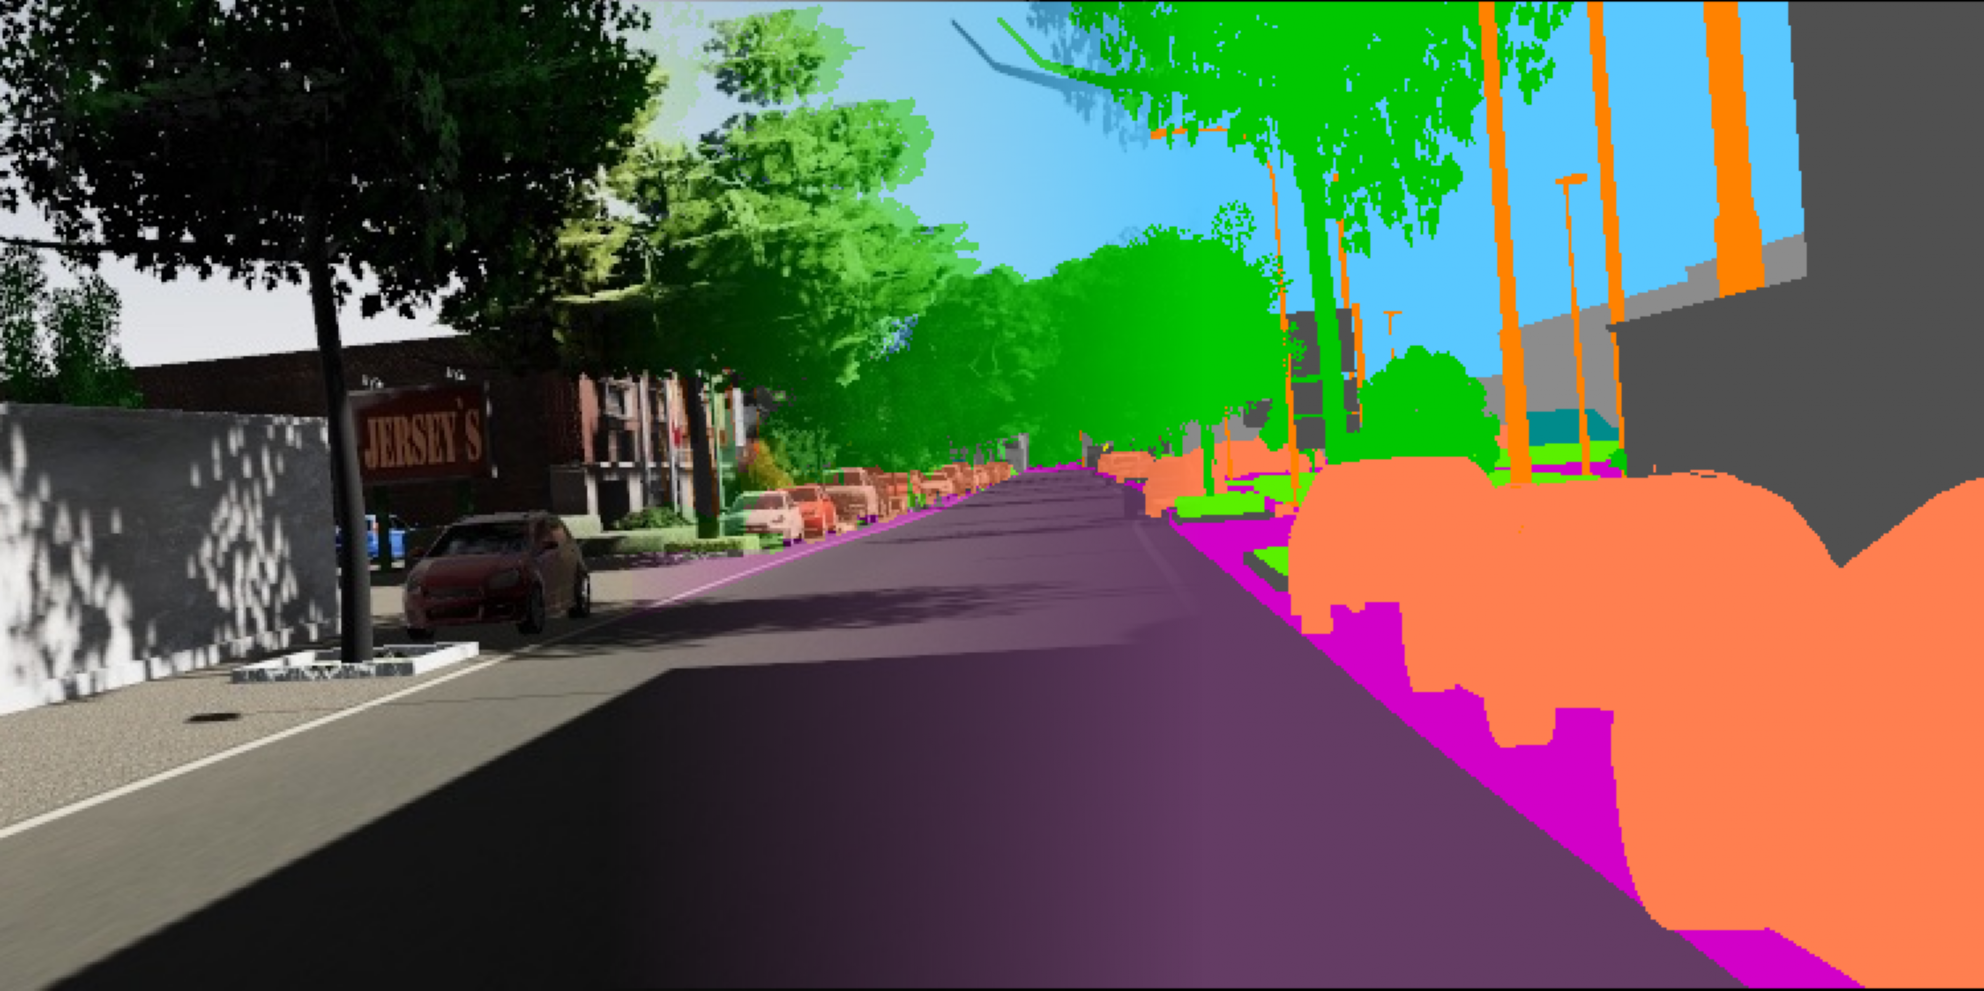
\includegraphics[width=\columnwidth]{img/2-related-work/virtual-kitti_semantic_segmentation_overlay.png}
    \caption {Virtual KITTI \cite{kitty}}
    \label{fig:example-virtual-kitti}
  \end{subfigure}

  \caption[Visual examples of synthetic datasets for urban scenes]{Visual examples of synthetic datasets for urban scenes}
    \label{fig:synthetic-datasets-examples}

\end{figure}

%%%%%%%%%%%%%%%%%%%%%%%%%%%%%%%%%%%%%%%%%%%%%%%%%%%%%%%%%%%%%%%%%%%%%%%%%%%%
%%%%%%%%%%%%%%%%%%%%%%%%%%%  GENERATIVE MODELS   %%%%%%%%%%%%%%%%%%%%%%%%%%%
%%%%%%%%%%%%%%%%%%%%%%%%%%%%%%%%%%%%%%%%%%%%%%%%%%%%%%%%%%%%%%%%%%%%%%%%%%%%

\section{Generative models}
Generative models, particularly those based on neural networks for the generation of new images, have gained significant popularity recently. Unlike discriminative models, which focus on learning the conditional distribution $P(Y|X)$ of output data Y given input data X, generative models aim to learn the joint distribution $P(X,Y)$.

For instance, consider a style transfer problem such as the one proposed in \cite{GUO2020127},  where an image from an urban environment simulator is enhanced to improve its photorealism. A generative model attempts to learn the probability distribution of $(X_i, Y_i)$ pairs, where $X_i$ is an input image and $Y_i$ is an improved version of the image. By sampling an element from the learned distribution of $Y$, a generative model can produce an image that fits within the given domain. Using this approach, generative models can be used to solve tasks such as style transfer, data augmentation, or synthetic data generation.

In contrast, discriminative models concentrate on learning the conditional distribution $P(Y|X)$ to make predictions based on input data $X$. In a classification-like problem, this is done by learning the boundary decision that separates different classes of $Y$ based on the input $X$. For example, in semantic segmentation, a discriminative model predicts the probability of semantic classes based on an input image $X_i$. Although discriminative approaches are very effective for tasks such as classification or regression, they are not suitable for generating new samples by sampling the learned distribution.

In Computer Vision, generative models have advanced significantly due to the availability of large computational resources and datasets with billions of images \cite{schuhmann2022laionb}, which have enabled the training of deep generative models. The design of models with controllable latent spaces has been a key factor in this evolution \cite{Asperti2022}. Latent spaces are low-dimensional representations learned from the input data that capture their underlying structure. By manipulating the values of these latent variables, the generative model can control specific aspects of the output or generate mixtures of output samples \cite{shen2020interpreting}.

Another significant development has been the creation of conditional generative models, which introduce a third element such as a text prompt to guide the generation of samples in a more direct way. This has led to the development of generative models that generate images \cite{rombach2022high, Dalle2}, audio \cite{liu2023audioldm}, or video \cite{ho2022imagen} based on natural language descriptions.

In the following subsections, we review the main architectures that have contributed to the development of generative models and have led to the design of diffusion models\cite{HoEtAl2020}. We pay special attention to the Stable Diffusion architecture \cite{rombach2022high}, which is the focus of this work.


\subsection{Generative architectures}

Deep generative models have achieved impressive results by learning a compact, expressive latent space that enables better synthesis or manipulation of high-dimensional data. However, developing generative architectures has been more challenging than their discriminative counterparts, given the complexity of the task. Nevertheless, machine learning's historical roots in classical architectures like Boltzmann machines \cite{ackley:boltzmann} or autoencoders \cite{rumelhart:errorpropnonote, ballard:modular} provided a foundation for the evolution of these models.

\subsubsection{Autoencoders}

\begin{figure}
    \centering
    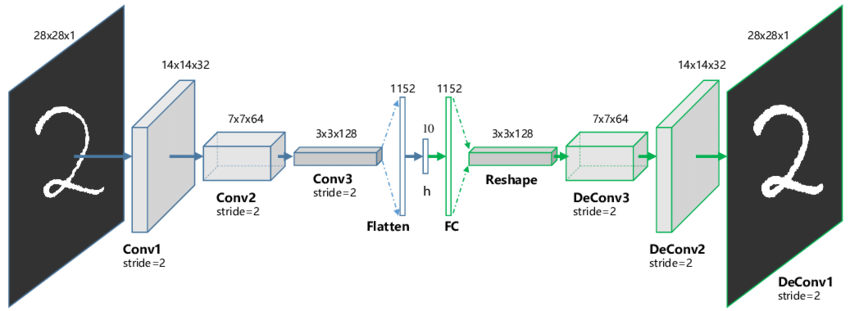
\includegraphics[width=0.8\columnwidth]{img/2-related-work/convolutional-autoencoder.png}
    \caption[Convolutional Autoencoder example]{Convolutional Autoencoder example. Source \cite{neurips/convolutionalautoencoders}.}
    \label{fig:Autoencoder}
\end{figure}


Autoencoders, which date back to the 1980s \cite{rumelhart:errorpropnonote, ballard:modular}, are neural architectures in which a bottleneck layer with a small number of neurons is introduced. In their original design, the network is trained to predict the same output example as the one given as input, but due to the bottleneck layer, a compact representation is forced to be learned. Figure \ref{fig:Autoencoder} shows an example of a Convolutional Autoencoder \cite{neurips/convolutionalautoencoders} following this scheme, which is trained to generate the same digit given as input but with a layer in the middle.

To increase the robustness of the learned representation, researchers have proposed different strategies. For example, Denoising Autoencoders \cite{conf/icml/VincentLBM08} introduce noise in the input samples, Contractive Autoencoders \cite{conf/icml/RifaiVMGB11} include penalty terms, or other works proposed the learning of more complex unsupervised tasks \cite{IEEE/Pathak2016, ieee/zhang2017, Shu_2018_ECCV}.

Autoencoders have been successfully applied to reconstruct noisy images \cite{conf/icml/VincentLBM08} and perform style transfer tasks such as image colorization \cite{zhang2016colorful}. However, when used for generating new synthetic samples using new values of the learned latent space representation in the bottleneck layer, the generated samples may lack variability. Additionally, the learned space may not exhibit desirable properties, as interpolation in the space does not always produce high-quality samples. As a result, other architectures such as Generative Adversarial Networks \cite{NIPS2014_5ca3e9b1} or Latent Diffusion models have become more popular in these types of applications.

\subsubsection{Generative Adversarial Networks (GANs)}

%\begin{figure}
%    \centering
%    \includegraphics[width=0.9\columnwidth]{img/2-related-work/gan-%design.png}
%    \caption[TDiagram of a GAN]{Diagram of a GAN.}
%    \label{fig:gan}
%\end{figure}


%\begin{figure}
%    \centering
%    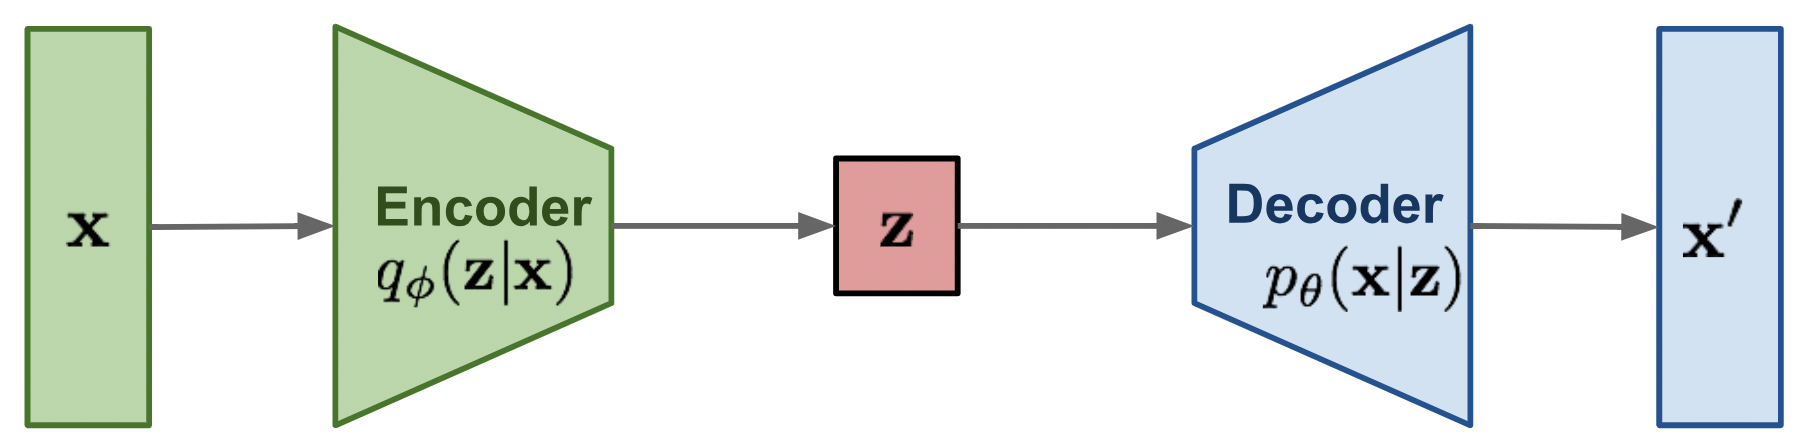
\includegraphics[width=0.9\columnwidth]{img/2-related-work/vae-design.png}
%    \caption[Variational Autoencoder architecture]{Variational Autoencoder architecture \cite{Asperti2021}}
 %   \label{fig:vae}
%\end{figure}

Generative Adversarial Networks (GANs) \cite{NIPS2014_5ca3e9b1} were proposed in 2014 as a revolutionary idea in deep learning, inspiring research in the field ever since. GANs are composed of two neural networks - a generator network $G$ and a discriminator network $D$. The generator network is trained to generate synthetic samples $x'$ from a latent vector $z$ from a known distribution, such as a Gaussian noise distribution. Meanwhile, the discriminator network is trained to classify synthetic and real samples, distinguishing between them. Figure \ref{fig:gan} provides an illustration of this architecture.

The training of GANs is formulated as a search for a Nash equilibrium in a zero-sum game, in which the discriminator seeks to minimize its cost function $J^{(D)}$, while the generator tries to maximize it. The original formulation of $J^{(D)}$ is defined as

\begin{equation}
J^{(D)}(\theta^{(D)}, \theta^{(G)}) = - \frac{1}{2} \mathbb{E}_{x \thicksim X } \log D(x) - \frac{1}{2} \mathbb{E}_{z} \log (1 - D(G(z))).
\end{equation}

However, this theoretical definition is not very practical for training, so variations of the cost functions were proposed to make the training process more stable, but with the same underlying idea \cite{journals/corr/abs-1711-10337}. Even with these modifications, GAN training is dynamic and sensitive to nearly every aspect of its setup, so additional training strategies have been proposed to make them more stable. For example, Progressive GANs \cite{karras2018progressive} have been proposed to improve the stability of GAN training, increasing iteratively the number of layers of the networks during the training epochs. Additionally, strategies to condition generation and gain control in the synthetic samples created have been proposed \cite{radford2015unsupervised, NIPS2016_8a3363ab, conf/nips/ChenCDHSSA16}.


Despite their difficult training process, GANs are one of the most widely used architectures for generative tasks today. One of the reasons for their popularity is the desirable properties of their latent space, which allows for the varied generation of new samples and their control \cite{shen2020interpreting, radford2015unsupervised}. GANs have been successfully applied to a wide range of applications in Computer Vision, including image synthesis \cite{NIPS2016_8a3363ab}, image-to-image translation \cite{Isola2017}, and generation of images from segmentation masks \cite{Wang2018, Park2019}. They have also been applied to video synthesis \cite{wang2018-video} and other applications in natural language processing and signal processing.


\subsubsection{Variational Autoencoders (VAEs)}



\begin{figure}
    \centering
    \begin{subfigure}[b]{0.9\columnwidth}
    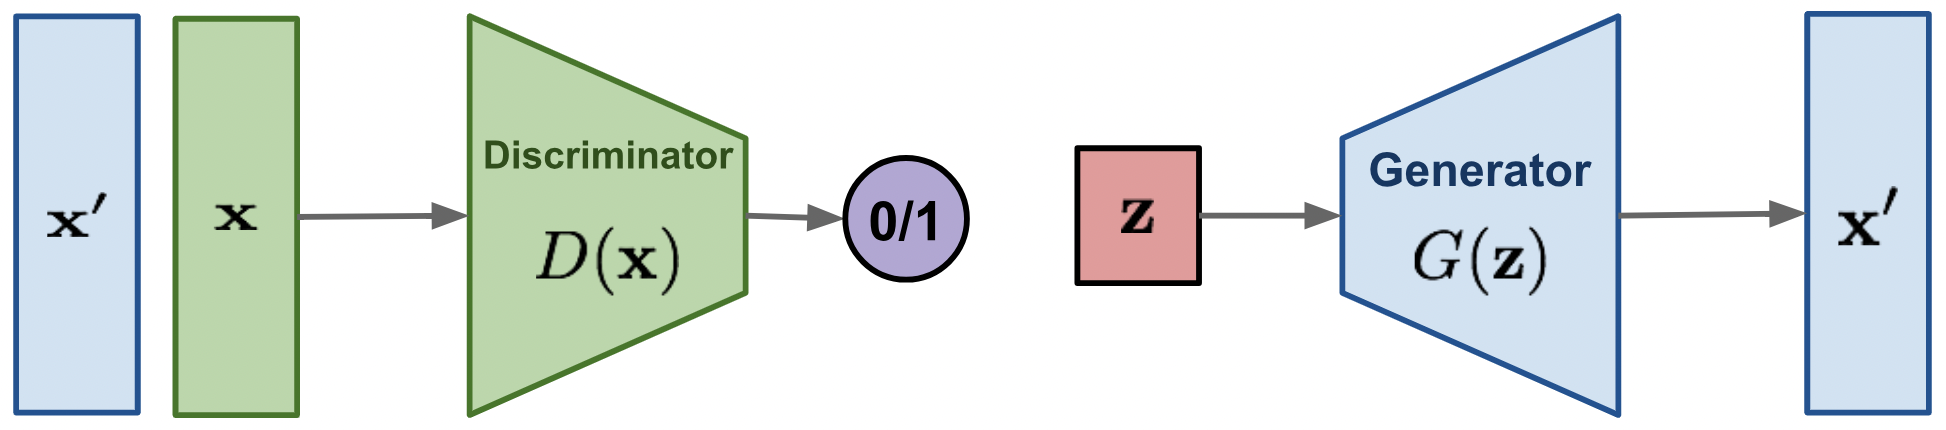
\includegraphics[width=\columnwidth]{img/2-related-work/gan-design.png}
        \caption{GAN Architecture}
        \label{fig:gan}
      \end{subfigure}

  
  \begin{subfigure}[b]{0.9\columnwidth}
    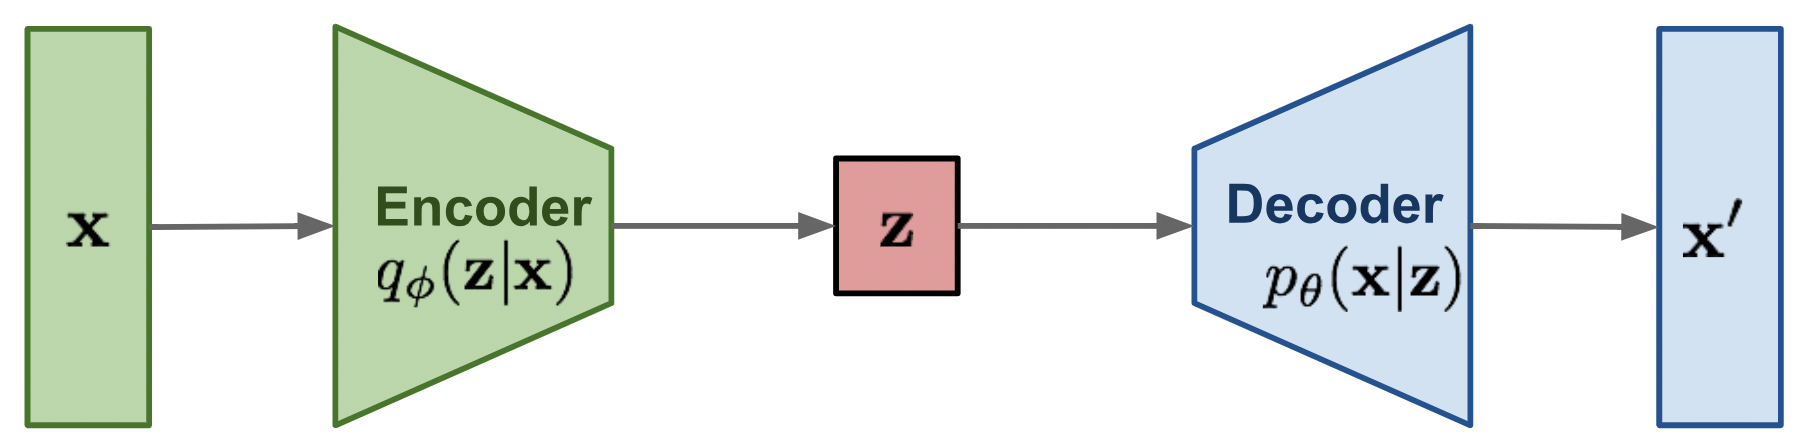
\includegraphics[width=\columnwidth]{img/2-related-work/vae-design.png}
    \caption{VAE Architecture}
    \label{fig:Vae}
  \end{subfigure}
    \caption[VAE and GAN architecture]{VAE and GAN architecture. Source \cite{lilianweng}.}
    \label{fig:gan-vae}
\end{figure}


The Variational Autoencoder (VAE) is a generative model introduced in 2014 \cite{Kingma2014}. Traditional autoencoders can encode input samples into a latent representation in the bottleneck, which can then be used to reconstruct the original input. However, they lack variability in their generated samples, making them less suitable for content generation. The VAE is an extension of traditional autoencoders with a similar encoder-decoder structure, but it adds a probabilistic layer to the encoder. The encoder transforms the input samples into the parameters of a variational distribution, allowing for the generation of new content by sampling from the learned distribution in the latent space. The decoder takes a latent value sampled from the learned distribution and transforms it into the output space.

To train the VAE, the model maximizes the Evidence Lower Bound (ELBO) of the data given the model parameters, which involves computing the reconstruction loss and the Kullback-Leibler divergence between the learned distribution and a prior distribution \cite{Asperti2021}. Thus, the training problem is defined as the maximization of the ELBO, which is formulated as:


\begin{equation}
    L_{\theta, \phi} (x) = \ln p_\phi (x) - D_{KL} (p_\phi(\cdot \, | \, x)\, \| \, q_\theta (\cdot \, | \, x)  )
\end{equation}


The VAE has played an important role in the current revolution of synthetic image generation, with important works such as the VQ-VAE \cite{NIPS2017_7a98af17}, the basis of DALL·E \cite{dalle1}, one of the text-to-image models that preceded the most popular architectures currently employed based on diffusion models \cite{Dalle2, rombach2022high}, in which is also a key component.

\subsection{Diffusion Models}
\label{sec:diffusion-models}

Diffusion Models, specifically Denoising Diffusion Probabilistic Models (DDPMs), are a type of latent generative model proposed in 2020 \cite{HoEtAl2020}. Their main purpose is to generate high-quality samples from a given distribution. DDPMs are based on an iterative process inspired by non-equilibrium thermodynamics, which involves applying a chain of diffusion steps that gradually introduce random noise to the input data. Although diffusion models based on this concept have been proposed before \cite{pmlr-v37-sohl-dickstein15}, the approach of the DDPMs proposed in \cite{HoEtAl2020} enabled the subsequent development of the recently popular text-to-image architectures.


\subsubsection{Fordward diffusion process}

\begin{figure}
    \centering
    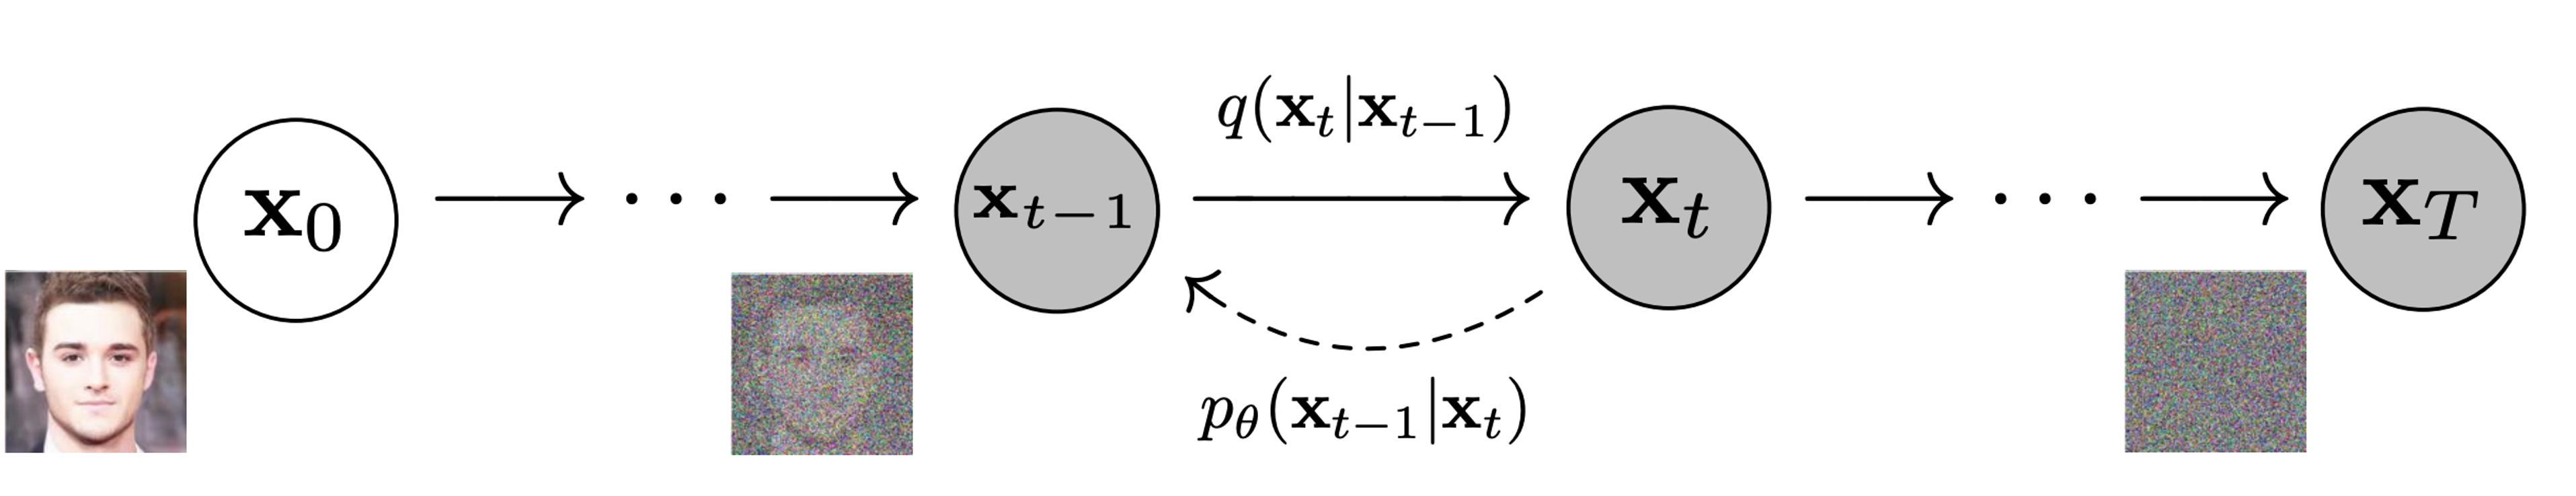
\includegraphics[width=1\columnwidth]{img/2-related-work/fordward-proccess.png}
    \caption[Forward diffusion process of a DDPM]{Forward diffusion process of a DDPM \cite{HoEtAl2020}.}
    \label{fig:fodward-diffusion-process}
\end{figure}

Figure~\ref{fig:fodward-diffusion-process} illustrates the forward diffusion process of a DDPM, in which a data point $\textbf{x}0 \sim q(x)$ from a distribution of input images is gradually transformed through a sequence of $T$ diffusion steps until the image become indistinguishable due to the noise. In its original formulation \cite{HoEtAl2020}, the diffusion process uses Gaussian noise with a predefined variance schedule $\{\beta_t \in (0, 1)\}_{t=1}^T$. When $T \rightarrow \infty$, the result of the process, $\textbf{x}_T$, is distributed as an isotropic Gaussian variable. With this formulation, for an arbitrary timestep $t$, the process $q$ is distributed as


\begin{equation}
    q(\textbf{x}_t |\textbf{x}_{t-1}) \sim \mathcal{N}\left(\sqrt{1 - \beta_t}\textbf{x}_{t-1}, \beta_t \textbf{I}\right).
\end{equation}

Employing a cumulative product of the timestep variances $\Tilde{\alpha}_t = 1 - \prod_{i=1}^t (1 - \beta_t)$, the distribution can be reparameterized in terms of the original input $\textbf{x}_0$ as


\begin{equation}
    q(\textbf{x}_t |\textbf{x}_{t-1}) \sim \mathcal{N}\left(\sqrt{1 - \Tilde{\alpha}_t}\textbf{x}_0,  \Tilde{\alpha}_t \textbf{I}\right).
\end{equation}

\subsubsection{Reverse diffusion process}
 
If we could reverse the diffusion process and sample from $q(x_{t-1}|x_t)$, we could reconstruct the original sample from a noise input $\textbf{x}_T$. However, this inverse process is intractable, thus it is not possible to estimate it directly. Instead, we can train a model $p_\theta$ to approximately perform the inverse process using the Algorithm \ref{alg:training} described in \cite{HoEtAl2020}, in which the function $\epsilon_{\theta}$ learns to predict the noise $\epsilon$ added in a timestep from $\textbf{x}_t$.


\begin{multicols}{2}

\begin{algorithm}[H]
\caption{DDPM training}\label{alg:training}
\begin{algorithmic}
\Repeat
\State $\textbf{x}_0 \sim q(\textbf{x}_0)$
\State $t \sim \text{Uniform}(\{1, \ldots, T\})$
\State $\textbf{$\epsilon$} \sim \mathcal{N}(\textbf{0}, \textbf{I})$
\State Take gradient descent step on
\State \footnotesize{$\hspace{2em}  \nabla_\theta\left\| \textbf{$\epsilon$} - \textbf{$\epsilon$}_{\theta} \left(\sqrt{1 - \Tilde{\alpha}_t}\textbf{x}_0 + \sqrt{ \Tilde{\alpha}_t}\textbf{$\epsilon$}, \,t\right) \right\|^2$ }\normalsize{}
\Until converged
\end{algorithmic}
\end{algorithm}


\begin{algorithm}[H]
\caption{DDPM sampling}\label{alg:sampling}
\begin{algorithmic}
\State
\vspace{0.7em}
\State $\textbf{x}_T \sim \mathcal{N}(\textbf{0}, \textbf{I})$ 
\For{$t=T, \ldots , 1$}
\State $\textbf{z} \sim \mathcal{N}(\textbf{0}, \textbf{I})$ if $t>1$, else $\textbf{z}=\textbf{0}$
\State $\textbf{x}_{t-1} =$ \scriptsize{$\frac{1}{\sqrt{1 - \beta_t}} \left( \textbf{x}_t  - \frac{\beta_t}{\sqrt{ \Tilde{\alpha}_t}} \textbf{$\epsilon$}_\theta(\textbf{x}_t, t)   \right) + \sqrt{\beta_t} \textbf{z}$} \normalsize{}
\EndFor
\State \Return $x_0$
\end{algorithmic}
\end{algorithm}
\end{multicols}


The training algorithm, samples an initial data point $x_0$ from the input distribution $q(x_0)$ and a random timestep $t$ between 1 and $T$. Then, it samples a random vector \textbf{$\epsilon$} from the noise distribution. It takes a gradient descent step on the difference between \textbf{$\epsilon$} and $\textbf{$\epsilon$}_{\theta}$, evaluated at $(\sqrt{1 - \Tilde{\alpha}_t}\textbf{x}_0+\sqrt{\Tilde{\alpha}_t}\textbf{$\epsilon$}_t, t)$. The sampling process (Algorithm \ref{alg:sampling}), generates a sample $\textbf{x}_T$ from the noise distribution and performs a reverse diffusion process over $T$ timesteps using $\epsilon_\theta$ to obtain the reconstructed image.

In practice, several variations of the original proposal have been developed to address specific challenges and use cases. For instance, there have been introduced mechanisms for conditional generation \cite{Dhariwal2021} and the use of text as input \cite{Dalle2, rombach2022high}. In addition, other classes of noises, schedules, and losses are employed to improve the convergence of the inverse process modeling the noise as an ODE \cite{song2021scorebased}. However, diffusion-based models that have recently gained popularity, such as DALLE·2 \cite{Dalle2} or Stable Diffusion \cite{rombach2022high}, are based on the same underlying idea as above.

\subsubsection{Stable Diffusion}


Stable Diffusion \cite{rombach2022high} is a widely used latent diffusion model for image generation. Its open-source nature has allowed for the emergence of many research works exploring the architecture and a wide range of applications. The model has gained significant traction since its launch, thanks to the release of several pre-trained versions. In this work, we focus on the Stable Diffusion 2.0 version\footnote{Stable Diffusion 2.0: \href{https://huggingface.co/stabilityai/stable-diffusion-2}{huggingface.co/stabilityai/stable-diffusion-2} (Accessed June 2023).}, a 1.1 billion parameters version pre-trained on the LAION 5-billion image dataset \cite{schuhmann2022laionb}. The architecture is highly versatile, with variations that allow it to perform image manipulation tasks such as image inpainting, outpainting, and super-resolution. However, in this work we focus on the original text-to-image sampling mode.

The architecture comprises three main components: a deep language model to generate word embeddings, a VAE that encodes and decodes latent vectors into images, and a time-conditional denoising network responsible for denoising the latent models in the diffusion process. Additionally, some versions of the model include a final classifier to filter out Not Safe for Work (NSFW) content. A diagram illustrating the components of the model can be seen in Figure \ref{fig:stable-diffusion}.

The deep language model $\tau_{\theta}$, generally a CLIP model \cite{Radford2021LearningTV}, is responsible for transforming the input text prompts in natural language into word embeddings. These embeddings are vectors of fixed size in a more appropriate space in which there are preserved structures that maintain semantic relationships between words. These vectors are then used in the diffusion process to condition the generation by guiding the generated images by means of attention mechanisms. Generally, this language component is pre-trained separately and its weights are not modified during the training of the diffusion model \cite{dosovitskiy2020vit}.

The conditional denoiser network $\epsilon_{\theta}$, generally a conditional U-NET as in Stable Diffusion 2, is in charge of performing the iterative process of inverse diffusion. Unlike the original U-NET \cite{UNET} (see Figure~\ref{fig:unet}), a variation is used in which cross-attention layers are introduced, in charge of introducing the information of the text embeddings to guide the denoising process. Later, in Section \ref{sec:explainability-dm}, we dwell on these attention mechanisms, since we extract from them the information of the semantic segmentation masks during the generation of synthetic images.

The VAE \cite{Kingma2014} is formed by an encoder $\mathcal{E}$ and a decoder $\mathcal{D}$ (see Figure \ref{fig:Vae}). The encoder $\mathcal{E}$ is in charge of transforming images to the latent space of the network where the diffusion process is applied. Although the encoder is mainly used for training the architecture, it can be used in the sampling process to initialize the diffusion process with an image. The VAE decoder $\mathcal{D}$ transforms the U-NET output after applying the inverse diffusion process to convert the denoised latent variable $z$ into an image.

\begin{figure}
    \centering
    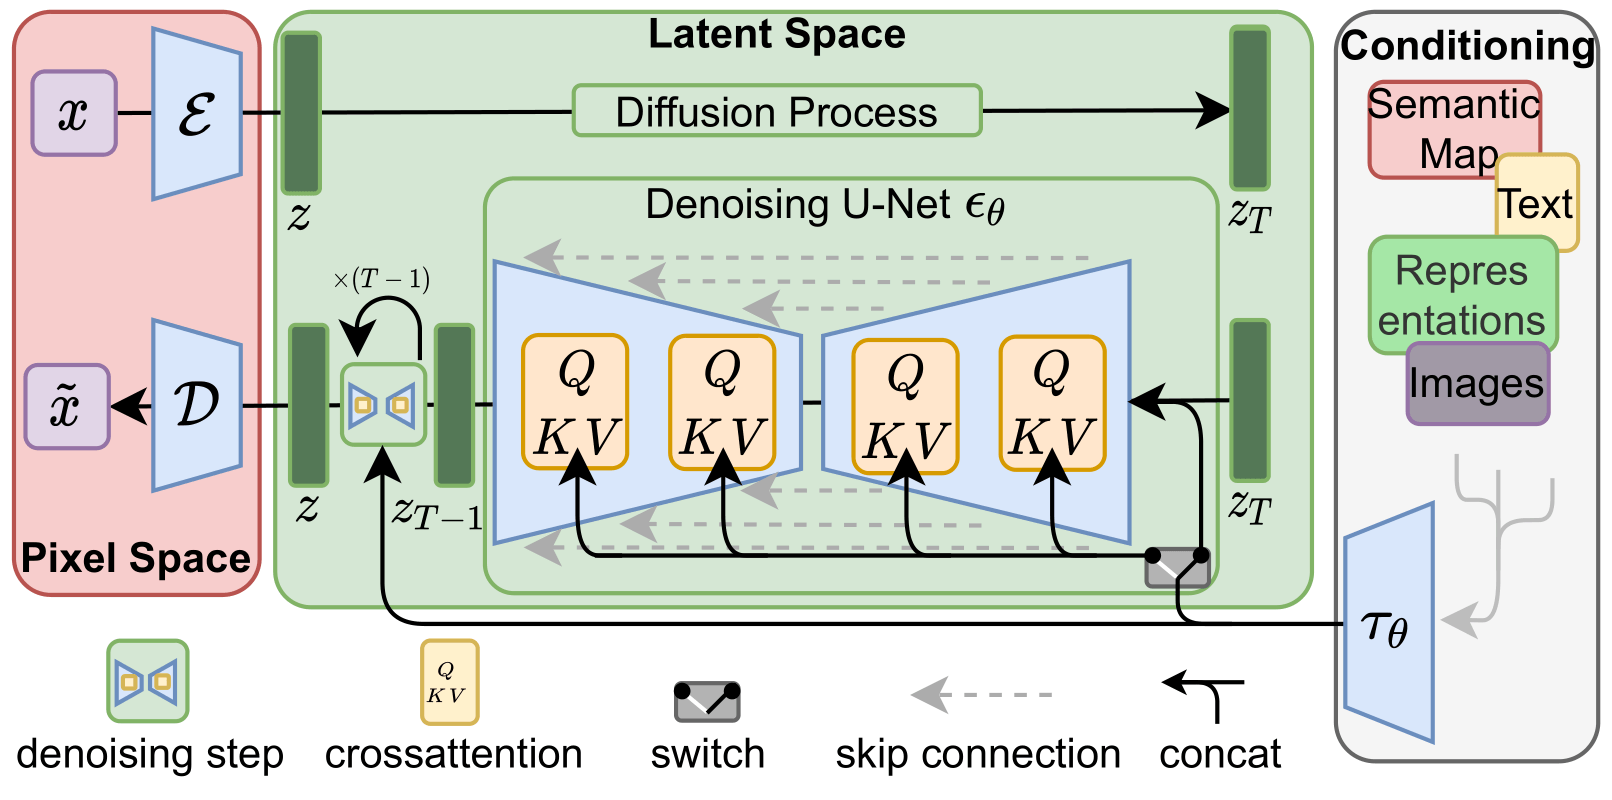
\includegraphics[width=\columnwidth]{img/2-related-work/stable-diffusion-architecture.png}
    \caption[Stable Diffusion architecture]{Stable Diffusion architecture. Source \cite{rombach2022high}.}
    \label{fig:stable-diffusion}
\end{figure}


\subsubsection{Challenges in Synthetic Data Generation using Stable Diffusion}
%Nota: En esta sección añadiré los diferentes avances que aparezcan en SD. Como text-to-video, reinforcement learning, text-to-audio, cambio de losses, etc... Como varia semana a semana lo cambiaré al final con lo que haya resultado más trascendente en los próximos meses.

Despite the progress made in text-to-image generation, there are still several challenges that need to be addressed. One major challenge is the difficulty of generating images that accurately match the input text. This is particularly challenging when dealing with too specific concepts or complex scenes that require a high level of visual understanding.

Several methods have been proposed to address this challenge, including the use of additional constraints on the architecture to respect a predefined structure, such as a given segmentation map, during image generation \cite{zhang2023adding}. Other works focus on adjusting the attention generated on the cross-attention layers during image generation to mitigate the model from discarding part of the text information given as input \cite{AttendAndExcite}.

Improving the accuracy of text prompts is also an important issue that has been addressed in recent works. The term \emph{prompt engineering} has become popular to describe the optimization of queries to improve image generation \cite{promptEngineering}. Among the lines of research focused on automating this process, we can highlight works focused on obtaining queries that generate images as similar as possible to a given image \cite{HardPromptsMadeEasy} or the use of reinforcement learning to train systems capable of generating better text prompts \cite{Promptist}. These methods can significantly improve the generation of high-quality images from text without modifying the text-to-image architecture.

All these challenges motivate the development of methods for the explainability of latent diffusion image generation. A better understanding of the underlying processes allows for the creation of text prompts that are better suited to generate images, as well as the development of more sophisticated techniques to interact with these models. 
These topics are explored in more detail in Section \ref{sec:explainability}.


%%%%%%%%%%%%%%%%%%%%%%%%%%%%%%%%%%%%%%%%%%%%%%%%%%%%%%%%%%%%%%%%%%%%%%%%%%%%
%%%%%%%%%%%%%%%%%%%%%%%%%%%%%  EXPLAINABILITY   %%%%%%%%%%%%%%%%%%%%%%%%%%%%
%%%%%%%%%%%%%%%%%%%%%%%%%%%%%%%%%%%%%%%%%%%%%%%%%%%%%%%%%%%%%%%%%%%%%%%%%%%%

\section{Explainability}
\label{sec:explainability}

The rise of Deep Learning has paved the way for remarkable advances in Computer Vision, enabling us to solve tasks that would have been difficult to tackle in the past \cite{Chai2021}. However, the increasing complexity of these models and their widespread use across various domains have brought new challenges. One such challenge is the lack of transparency and interpretability in these models, which can hinder their potential applications in real-world scenarios.

Traditionally, these models have been treated as a black box, with little attention paid to their internal workings. However, this approach presents significant limitations, as it becomes difficult to explain how the model arrived at a particular decision. Furthermore, the lack of transparency in these models poses legal and ethical risks, as accountability becomes challenging when the decision-making process is not transparent \cite{Gerlings2020ReviewingTN}.

To address these issues, the field of explainable Artificial Intelligence (\emph{XAI}) has emerged, aiming to develop methods that make these models more transparent and interpretable \cite{SALEEM2022165}. This is particularly relevant in Computer Vision \cite{QuanshiZHANG}, where interpretability and explainability can be fundamental for understanding the inner workings of models and addressing issues such as bias and fairness \cite{Kirill2022}.


While the terms explainability and interpretability are often used interchangeably due to their close relation, they are distinct tasks. Interpretability measures the extent to which a model can associate a cause with an effect, based on its input and output variables. For instance, \emph{Shapley values} can be used to assign a numeric weight to each input variable, reflecting its influence on an output prediction \cite{shapley}. On the other hand, explainability is a broader task that pertains to the ability of a model's decisions to be understood by humans, including the ability to describe the model's behavior and the factors that influence it \cite{Gerlings2020ReviewingTN}. For example, an explanation of a model's behavior might involve identifying specific features in an input image that caused the model to produce a particular output prediction \cite{extremalPerturbations}. Alternatively, it could entail identifying which features activate a certain layer or node of a neural network, providing insights into the hierarchy of features used by the network \cite{optimizationInput}, and identifying potential biases in the model.

In this section, we explore the issue of explainability in Computer Vision, focusing specifically on diffusion models. We begin by reviewing the concept of explainability in Computer Vision and the main methods currently employed. Next, we delve into the specific challenges related to the explainability of diffusion models, discussing recent developments and identifying potential avenues for future research. Finally, we discuss the relevance of explainability in the scenario of synthetic image generation for semantic segmentation, highlighting the significance of transparent and interpretable models in real-world applications.

\subsection{Explainability in Computer Vision}

\begin{figure}
\centering
 \begin{subfigure}{0.3\columnwidth}
    
\includegraphics[width=0.95\columnwidth, height=0.95\columnwidth]{img/2-related-work/bias-computer-vision-doctor.png}
    \caption{Original}
    \label{fig:biased-model-cam-image}
  \end{subfigure}
  \begin{subfigure}{0.3\columnwidth}
    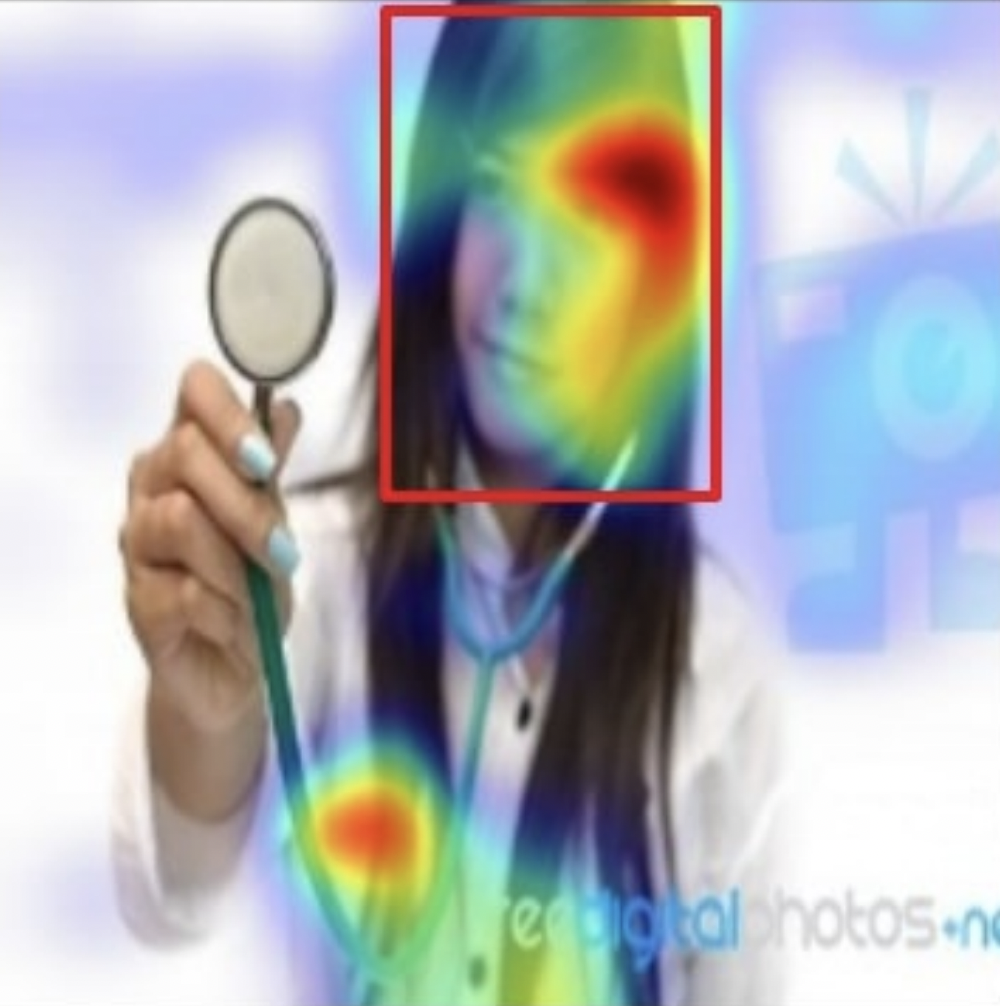
\includegraphics[width=0.95\columnwidth, height=0.95\columnwidth]{img/2-related-work/bias-computer-vision-doctor-nurse.png}
    \caption{CAM of ``Nurse''}
    \label{fig:biased-model-cam-nurse}
  \end{subfigure}
  \begin{subfigure}{0.3\columnwidth}
    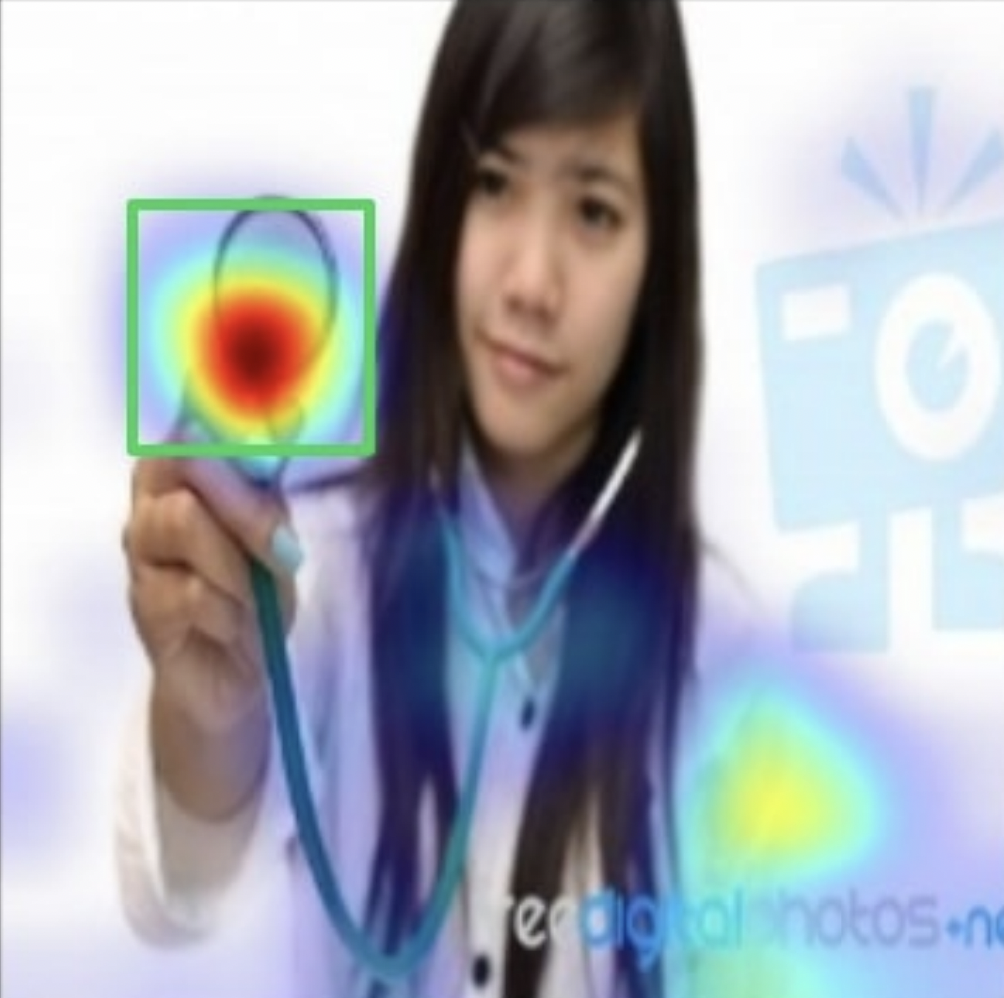
\includegraphics[width=0.95\columnwidth, height=0.95\columnwidth]{img/2-related-work/bias-computer-vision-doctor-cam.png}
    \caption{CAM of  ``Doctor''}
    \label{fig:biased-model-doctor}
  \end{subfigure}

  \caption[Class activation maps (Grad-CAM) of a biased model]{Class activation map (Grad-CAM) of a biased model. (a) A stock photo image labeled as ``Doctor''. (b) Areas on which a biased model relies to predict the ``Nurse'' class (c) and ``Doctor''. Source \cite{gradcam}.}
  \label{fig:realbiased-model}
\end{figure}


\begin{figure}
\centering
 \begin{subfigure}{0.3\columnwidth}
    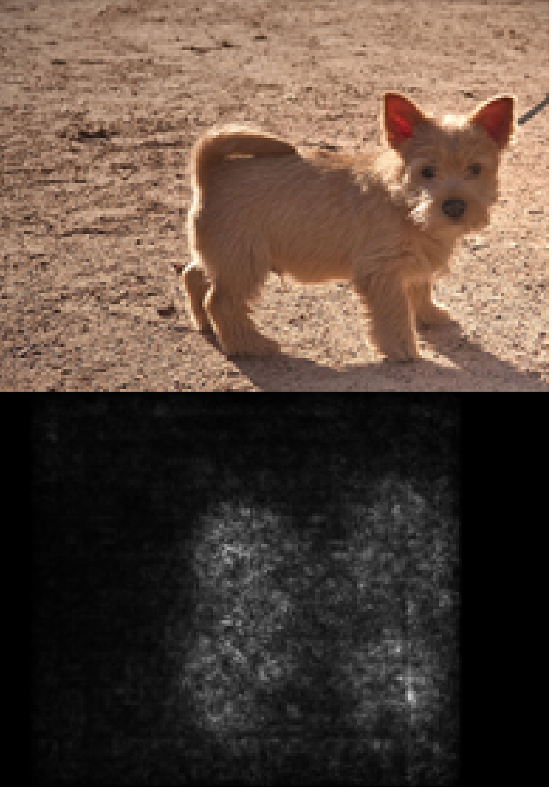
\includegraphics[width=0.95\columnwidth]{img/2-related-work/dog-saliency-map.png}
   %\caption{Saliency map \cite{Simonyan2013DeepIC}}
   \caption{}
    \label{fig:example-interpretability-1}
  \end{subfigure}
  \begin{subfigure}{0.3\columnwidth}
    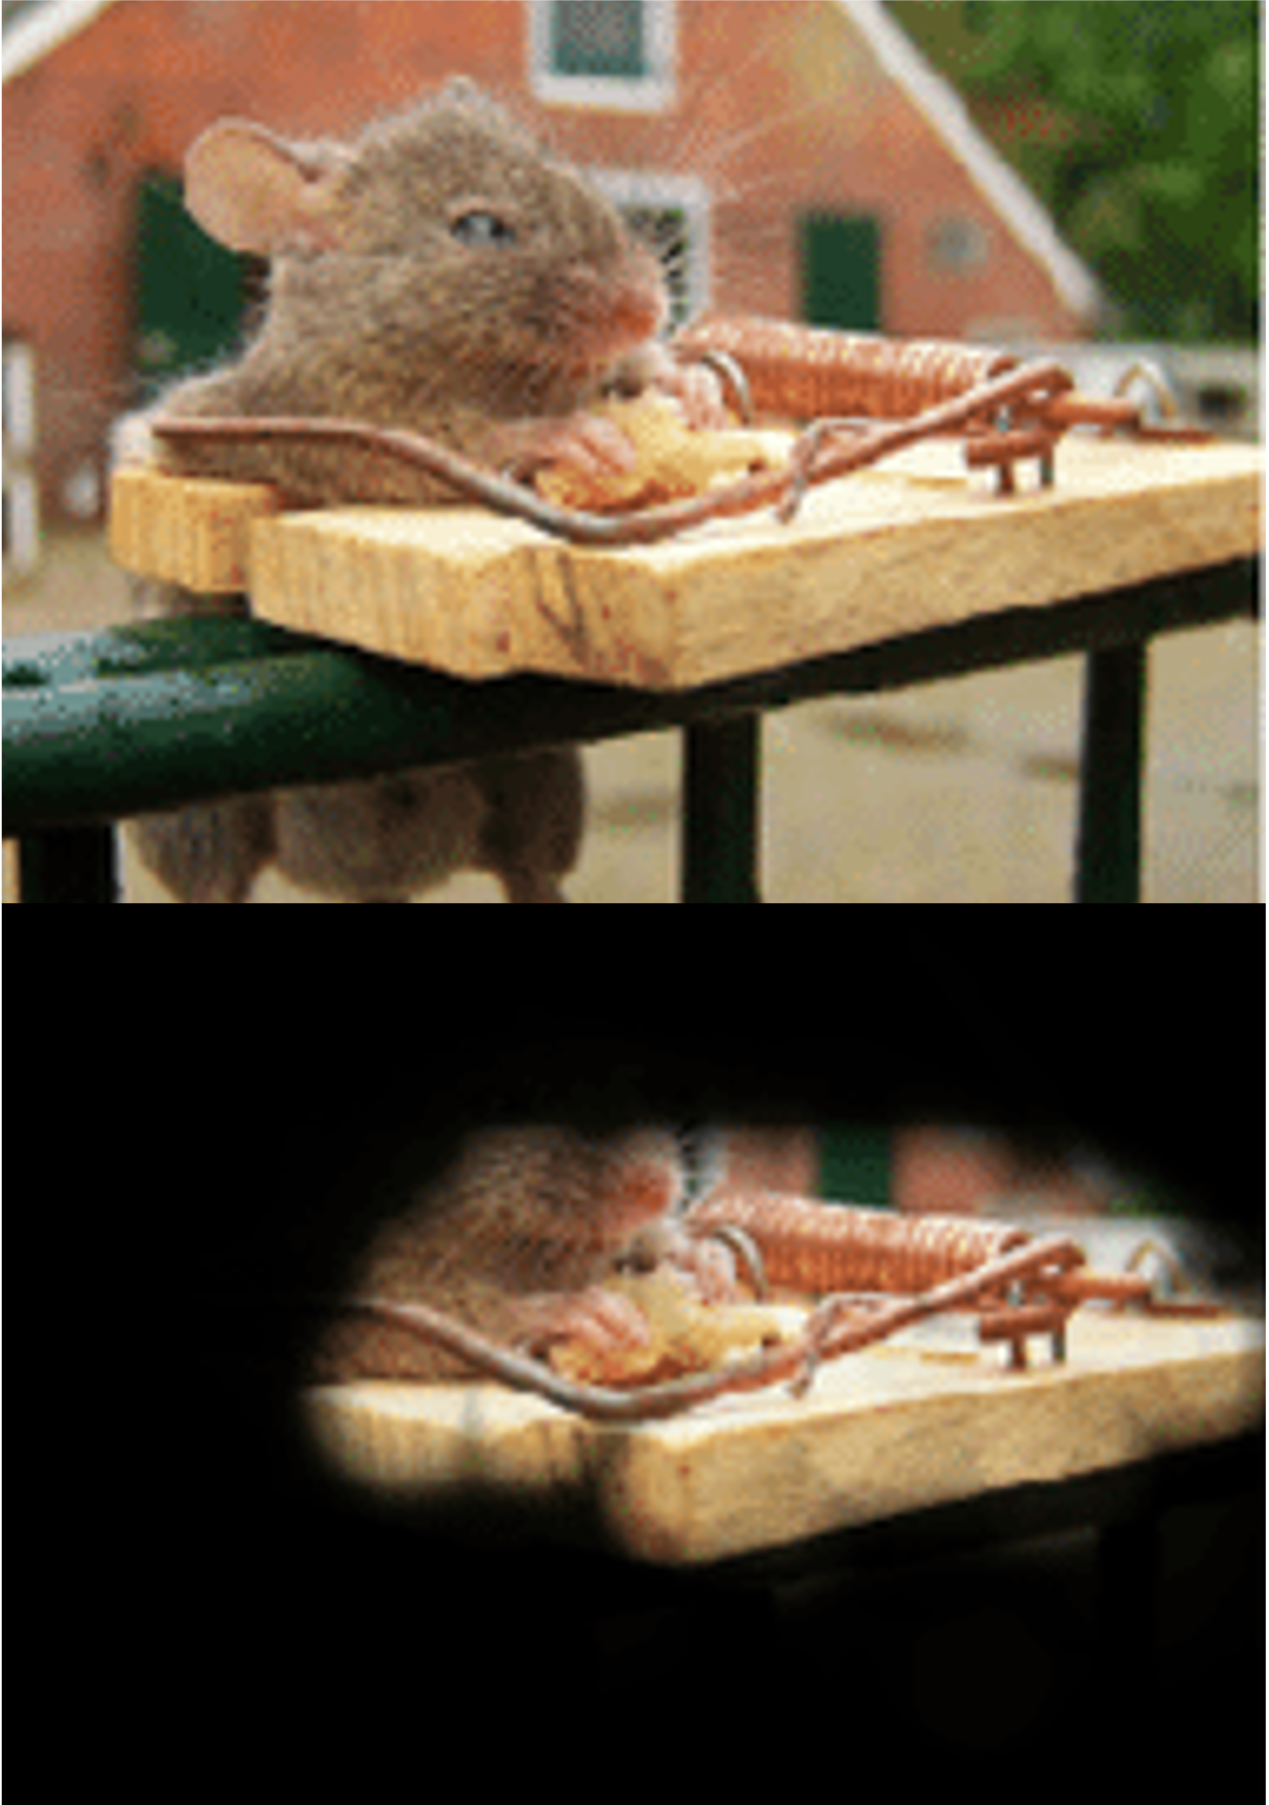
\includegraphics[width=0.95\columnwidth]{img/2-related-work/mouse-extremal-perturbations.png}
    %\caption{Extremal Perturbation \cite{Fong2019}}
    \caption{}
    \label{fig:example-interpretability-2}
  \end{subfigure}
  \begin{subfigure}{0.3\columnwidth}
    \includegraphics[width=0.95\columnwidth]{img/2-related-work/inceptionism.png}
    %\caption{Inception }
    \caption{}
    \label{fig:example-interpretability-3}
  \end{subfigure}
  \caption[Examples of explainability methods for Computer Vision]{Examples of explainability methods for Computer Vision. (a) Image of a dog and the corresponding Saliency Map \cite{Simonyan2013DeepIC} of the class ``Dog''. (b) Image of a mouse in a trap and a masked version using Extremal perturbations \cite{Fong2019} with the most discriminative part to classify the image as ``mouse trap''. (c) Feature optimization to maximize a convolutional layer response \cite{Mordvintsev2015InceptionismGD} using an image of a savanna as prior. The processed image contains more highlighted edges, indicating that the layer is activated in the presence of this type of low-level feature. Source \cite{Simonyan2013DeepIC, Fong2019, Mordvintsev2015InceptionismGD}.}
  \label{fig:example-interpretability}
  \end{figure}

Explainability methods for Computer Vision are becoming increasingly important due to regulatory requirements and the need for increased reliability \cite{Gerlings2020ReviewingTN}. Computer vision models are particularly susceptible to acquiring biases present in the datasets on which they are trained \cite{Kirill2022, GeirhosRMBWB19}. Figure \ref{fig:realbiased-model} provides a striking example of this phenomenon, where an image labeled as ``Doctor'' (\ref{fig:biased-model-cam-image}) is accompanied by the regions on which a biased model relies to classify the image as "Nurse" (\ref{fig:biased-model-cam-nurse}) and ``Doctor'' (\ref{fig:biased-model-doctor}), both sex-agnostic classes \cite{gradcam}. Notably, the biased model places a disproportionate weight on the long hair region to classify the image as ``Nurse'', and on the stethoscope to classify it as ''Doctor``. Such biases can result in harmful outcomes in various scenarios and may adversely impact the model's performance. However, explainability methods can help to detect and mitigate the impact of these biases.

To achieve explainability in Computer Vision, researchers use established methods to interpret convolutional models. These methods can be classified into three main approaches: gradient-based attribution methods, perturbation-based methods, and techniques for feature visualization using optimization techniques.

Gradient-based attribution methods are commonly used in Computer Vision to determine the contribution of each input feature to the final model prediction through the backpropagation of gradients. One such method is saliency maps \cite{Simonyan2013DeepIC}, which calculate the gradient of a class score with respect to the input image, highlighting the aspects that most influence the image's classification as that class (Figure \ref{fig:example-interpretability-1}). Other popular methods, such as Class Activation Maps (CAM) \cite{CAM} and Gradient-weighted Class Activation Mapping (GradCAM) \cite{gradcam}, use global average pooling in conjunction with gradient backpropagation to create class activation maps. These maps are heatmaps that identify the most relevant areas for classifying an image, as illustrated in Figure \ref{fig:realbiased-model}. These attribution maps can be used to detect potential biases in classification models and can even be used to perform object location and semantic segmentation of the object being classified.

Perturbation-based methods involve masking or altering input features to observe the effect on the model output. Examples of perturbation-based methods are Minimal Image Representation \cite{Zhou2014ObjectDE} and Extremal Perturbations \cite{Fong2019}, which attempt to learn a mask that removes parts of an image that have minimal impact on the output of a model, as illustrated in Figure \ref{fig:example-interpretability-2}. In contrast, other methods, such as Meaningful Perturbations \cite{Fong2017InterpretableEO}, try to blur or mask the parts of an image that most influence the model prediction.

Feature visualization methods are focused on understanding the behavior of neural networks by finding inputs that activate certain parts of the network through optimization. One commonly used technique is activation maximization, which involves maximizing the activation of a saliency map \cite{Simonyan2013DeepIC}. However, to make the obtained inputs more interpretable, additional methods like Feature Inversion \cite{featureInversion} or Inceptionism \cite{Mordvintsev2015InceptionismGD} utilize images as priors to generate more meaningful representations. By optimizing an input image that amplifies the activation of specific neurons in a neural network, we can obtain images that highlight the features that those neurons are encoding. This enables us to gain insights into whether a layer is filtering a specific texture or a semantic concept, as shown in Figure \ref{fig:example-interpretability-3}.

Explainability research in Computer Vision is currently a highly active field, with new techniques used in other domains still being explored, such as the use of counterfactual explanations \cite{conterfactual2019}, adversarial attacks \cite{Ghorbani_Abid_Zou_2019}, or causal reasoning \cite{Liu2022CausalRM}. While current methods have shown promise in detecting and mitigating biases in Computer Vision models, their application still poses several challenges. For example, there is a lack of consistency across techniques, which makes it difficult to compare and evaluate their interpretations. Measuring the effectiveness of these methods in practice is also complicated, especially when considering their impact on downstream tasks. Additionally, most established techniques are based on image classification, and extending them into generative tasks is still an emerging issue.

In recent years, explainability research has extended to other domains, such as natural language processing, where models such as transformers have been shown to achieve state-of-the-art performance on a variety of tasks but can be difficult to interpret \cite{attentionisnot,clark-etal-2019-bert}. One approach to interpretability in language models is to use attention mechanisms to visualize the words or phrases that the model is focusing on during prediction \cite{attentionisnot}. 

Overall, explainability methods are critical in ensuring the reliability and trustworthiness of machine learning models. As machine learning continues to be deployed in increasingly complex and sensitive applications, the development of effective and practical explainability methods will be essential for achieving transparency and accountability.


\subsection{Explainability of Diffusion Models}
\label{sec:explainability-dm}

The emergence of diffusion models for image generation is a relatively recent development, and research on methods for their explainability is still an emerging topic. Current research in this area focuses on text-attribution methods, which attempt to answer the question of which parts of an image are influenced most by each word in the text prompt. These methods aim to create heat maps of the influence of each word in the input text on the resulting image.

Unfortunately, early investigations in this direction found that methods based on gradients and perturbations cannot be adapted to diffusion models due to the iterative process involved in the diffusion process. Gradient methods require a backpropagation pass for every pixel for all $T$ time steps, which makes computation intractable and the process highly unstable. Perturbation-based methods result in significantly different images even with minor perturbations, making them unsuitable for diffusion models \cite{DAAM}.

As a result, the main methods being developed for explainability in diffusion models are based on ideas from natural language processing, where attention to words indicates lexical attribution \cite{clark-etal-2019-bert}. These methods exploit the conditional mechanisms based on cross-attention, where the text guides the image generation. One such method is the Diffusion Attentive Attribution Maps (DAAMs) \cite{DAAM}, whose maps are based on these attention mechanisms.

Other methods being explored for explainability in diffusion models involve modifying the attention process to highlight the attention of the tokens that need to be explained \cite{AttendAndExcite}, or by perturbing the attention \cite{deb2023atman}.

However, since this is still an emerging topic, many aspects remain to be investigated, and there are many potential issues that may expand the applications of these methods. In this work, we focus on exploring DAAMs for the extraction of semantic segmentation masks during synthetic image generation. As the DAAM method is important for our work, we provide a more detailed explanation of the process in Chapter \ref{cha:methodology}.




% https://github.com/heejkoo/Awesome-Diffusion-Models#inverse-problem			% incluir capítulo de estado del arte/state-of-art
\chapter{Proposed methods}
\label{cha:methodology}

This chapter introduces the theoretical framework that forms the core of this work, focused on the use of the attentions within LDMs for explainability purposes and their alignment with different objects in synthetically produced urban scenes.

Initially, in Section \ref{cha:methodology-daam}, we present the theory behind the DAAM explainability method \cite{DAAM}. This method allows the creation of attribution maps that relate the input text to the images generated by an LDM, further enabling the generation of segmentation masks. By attributing the influence of input tokens in the generated images, DAAM provides a valuable tool for understanding the connection between textual prompts and visual output.

Proceeding further, in Section \ref{cha:methodology-ov-daam}, we propose an extension of this explainability method, referred to as Open Vocabulary DAAM. This extension overcomes the limitation of the original DAAM by enabling the construction of attribution maps for any given text, not restricted to the tokens used during image generation. Open Vocabulary DAAM enhances the flexibility and applicability of the method, allowing for the exploration of diverse textual prompts and their influence on the generated images.

Finally, in Section \ref{cha:methodology-ov-daam-optimization}, we propose a methodology for optimizing an input text embedding to maximize the Intersection over Union (IoU) of DAAM-generated masks. This optimization process aims to align the generated masks more closely with the desired semantic segmentation masks, enhancing the fidelity and accuracy of synthetically generated ground truth.

Through this examination, we aim to cover the DAAM theoretical framework, its potential pitfalls, and paths for advancement. This foundation sets the stage for the empirical explorations presented in Chapter \ref{cha:experiments}, where we evaluate and analyze the practical implications of these methods on the task of semantic segmentation in urban scenes.

\section{Diffusion Attentive Attribution Maps}
\label{cha:methodology-daam}


The Diffusion Attentive Attribution Maps (DAAM) method represents a pioneering work in enhancing the explainability of text-to-image diffusion models \cite{DAAM}. This technique facilitates the attribution of individual input words' influence on the synthetic images generated by the model.

By leveraging the attention mechanisms activated during the diffusion process, 
DAAM constructs heatmaps corresponding to each token used as input.
These attention-based heatmaps align with semantically significant image areas, capturing not only primary objects but also abstract concepts embedded within the image, such as adjectives, verbs, or semantic relationships between words \cite{DAAM}.

For example, Figure \ref{fig:daam-example} presents an image generated with Stable Diffusion \cite{rombach2022high} using the text prompt ``A car in an urban environment'' (Figure \ref{fig:daam-example-image}), accompanied by DAAMs for each token in the prompt.  This prompt was chosen for this example after practical tests with various prompts, where it generated examples with a main object in the image within urban scenes, which aligns with the research context of this work. Each heatmap corresponds to a specific word in the input text, including the starting and ending special tokens, providing insights into how each word influences different regions of the generated image.
The following observations can be made from the heatmaps:


\begin{itemize}
\item \textlangle SOT\textrangle\ (\ref{fig:daam-example-image-1}): The heatmap primarily accumulates information from the image background, such as the city street and building. This attention pattern is common for the onset token, which tends to gather attention from regions not influenced by other tokens \cite{DAAM}.
\item ``a'' (\ref{fig:daam-example-image-2}): The heatmap exhibits a dispersed pattern across the entire image, suggesting that the word ``a'' influences various regions without a specific focus.
\item ``car'' (\ref{fig:daam-example-image-3}): The heatmap precisely outlines the shape of the car in the center of the image, highlighting the strong influence of the word ``car'' on that object.
\item ``in'' (\ref{fig:daam-example-image-4}): The heatmap focuses on the region of the car, indicating an semantic association between the word ``in'' and ``car''.
\item ``an'' (\ref{fig:daam-example-image-5}): The heatmap centers on the shape of the car but contains more noise, suggesting some ambiguity or uncertainty in the attribution.
\item ``urban'' (\ref{fig:daam-example-image-6}) and ``environment'' (\ref{fig:daam-example-image-7}): The heatmaps draw attention from various regions of the image, particularly the background building, indicating a strong association between these words and the elements of the environment.
\item \textlangle EOT\textrangle\ (\ref{fig:daam-example-image-8}): The heatmap complements the onset token's heatmap (\textlangle SOT\textrangle), with a specific focus on the car's location during the image generation process.
\end{itemize}


\begin{figure}
\centering
  % First column
  \begin{subfigure}{0.32\columnwidth}
   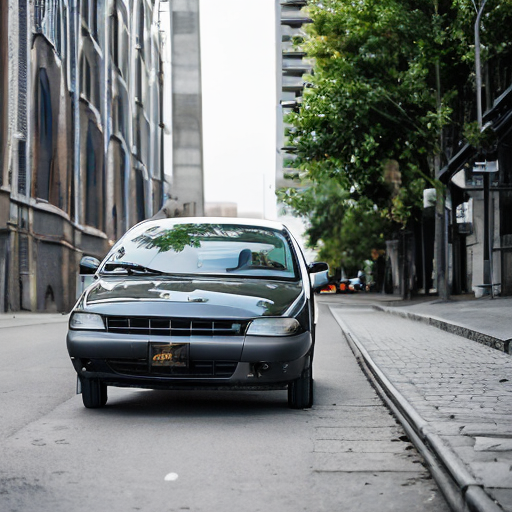
\includegraphics[width=\columnwidth]{img/3-methodology/example_daam.png}
   \caption{Image generated}
   \label{fig:daam-example-image}
  \end{subfigure}
  \begin{subfigure}{0.32\columnwidth}
   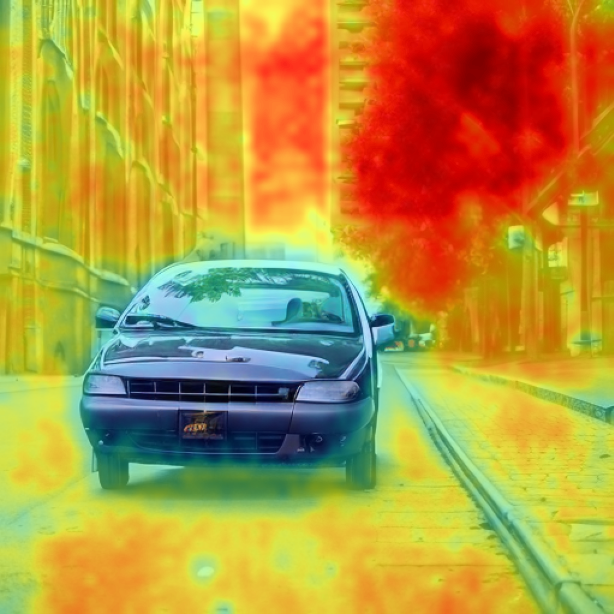
\includegraphics[width=\columnwidth]{img/3-methodology/example_daam_heatmap_SoT.png}
   \caption{\textlangle SOT\textrangle}
   \label{fig:daam-example-image-1}
  \end{subfigure}
  \begin{subfigure}{0.32\columnwidth}
   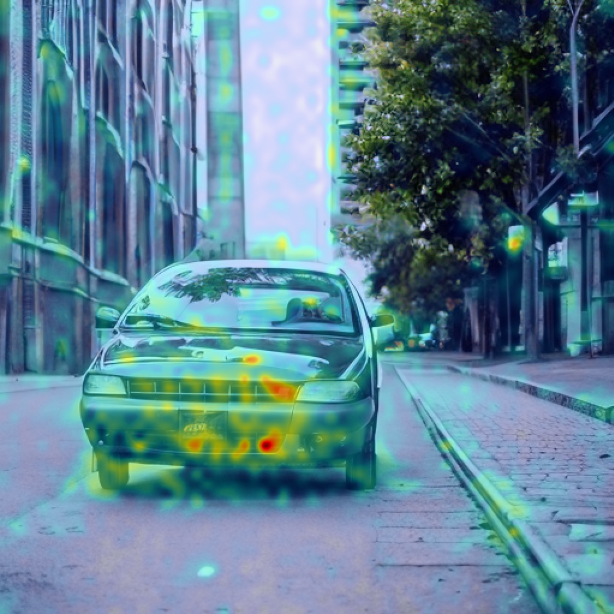
\includegraphics[width=\columnwidth]{img/3-methodology/example_daam_heatmap_a.png}
   \caption{``a''}
   \label{fig:daam-example-image-2}
  \end{subfigure}
  \par\bigskip
  % Second column
  \begin{subfigure}{0.32\columnwidth}
   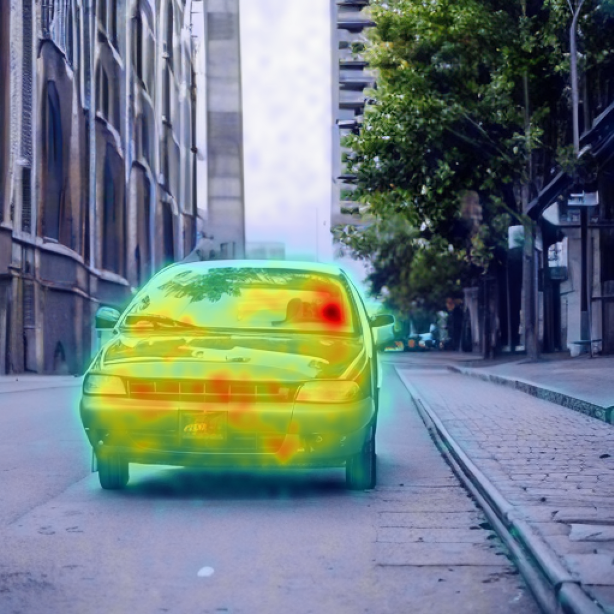
\includegraphics[width=\columnwidth]{img/3-methodology/example_daam_heatmap_car.png}
   \caption{``car''}
   \label{fig:daam-example-image-3}
  \end{subfigure}
  \begin{subfigure}{0.32\columnwidth}
   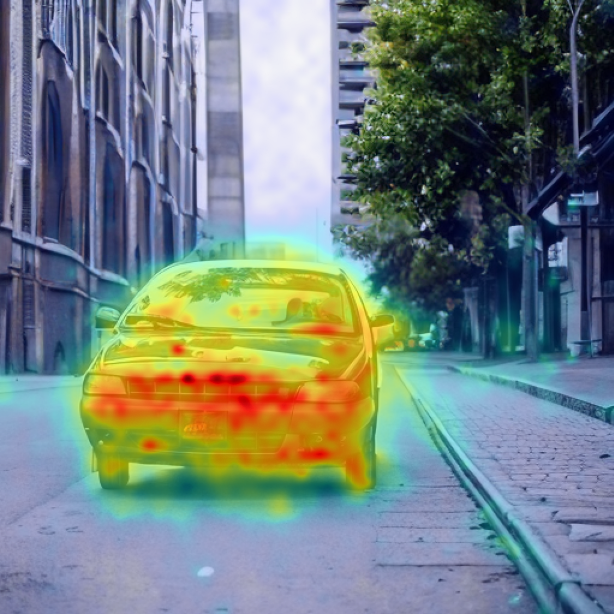
\includegraphics[width=\columnwidth]{img/3-methodology/example_daam_heatmap_in.png}
   \caption{``in''}
   \label{fig:daam-example-image-4}
  \end{subfigure}
  \begin{subfigure}{0.32\columnwidth}
   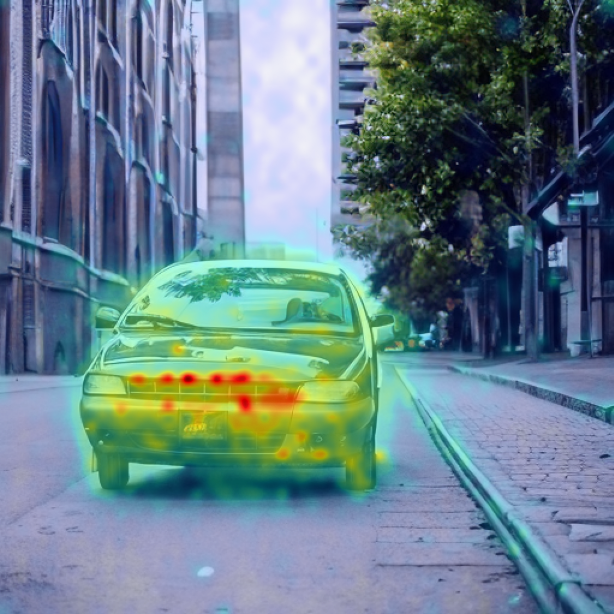
\includegraphics[width=\columnwidth]{img/3-methodology/example_daam_heatmap_an.png}
   \caption{``an''}
   \label{fig:daam-example-image-5}
  \end{subfigure}
  \par\bigskip
    % Third column
  \begin{subfigure}{0.32\columnwidth}
   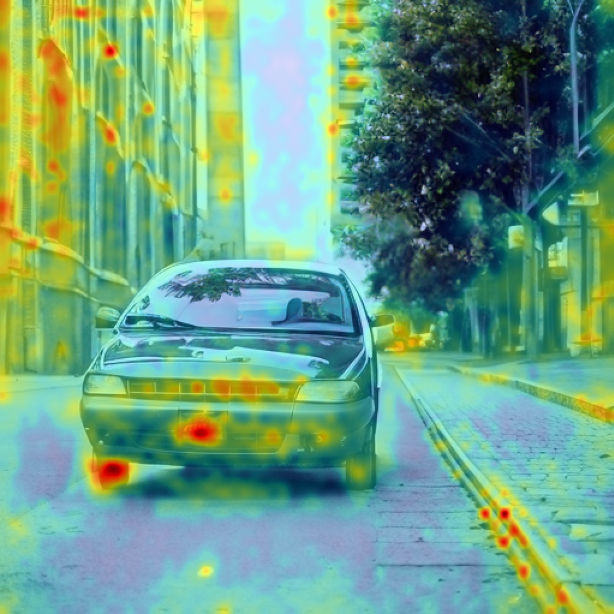
\includegraphics[width=\columnwidth]{img/3-methodology/example_daam_heatmap_urban.png}
   \caption{``urban''}
   \label{fig:daam-example-image-6}
  \end{subfigure}
  \begin{subfigure}{0.32\columnwidth}
   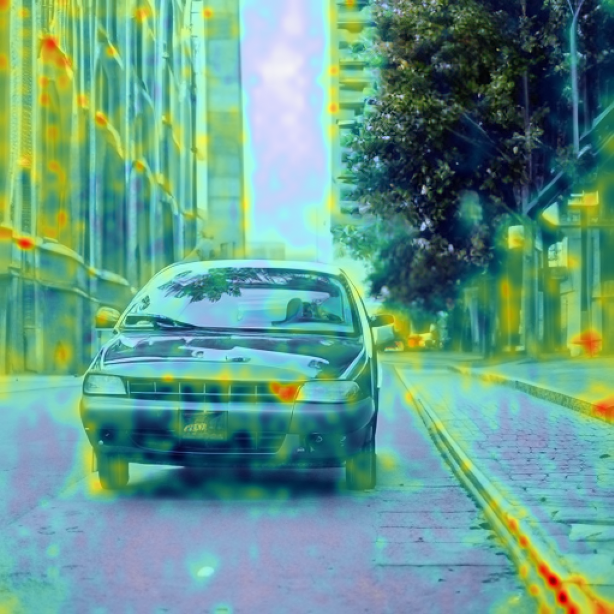
\includegraphics[width=\columnwidth]{img/3-methodology/example_daam_heatmap_environment.png}
   \caption{``environment''}
   \label{fig:daam-example-image-7}
  \end{subfigure}
  \begin{subfigure}{0.32\columnwidth}
   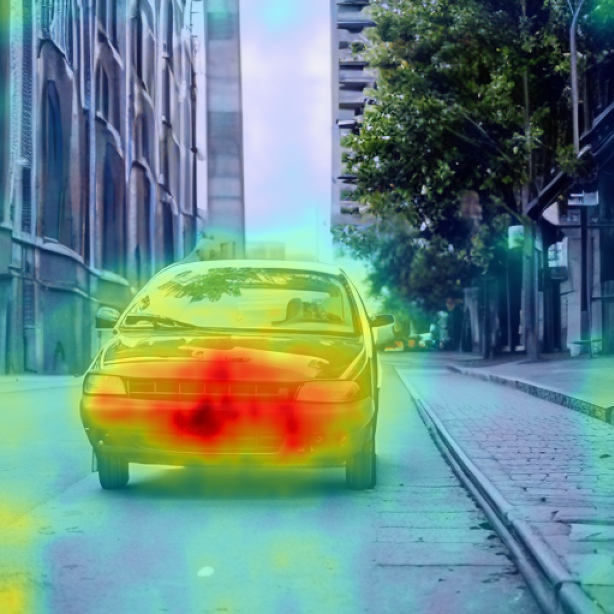
\includegraphics[width=\columnwidth]{img/3-methodology/example_daam_heatmap_EoT.png}
   \caption{\textlangle EOT\textrangle}
   \label{fig:daam-example-image-8}
   \end{subfigure}
  \caption[Example of Diffusion Attentive Attribution Maps]{An image generated using Stable Diffusion with the text ``A car in an urban environment'' along with overlayed DAAMs for each token.}
  \label{fig:daam-example}
  \end{figure}



This example illustrates the information provided by DAAM, revealing how each word influences distinct regions of the generated image. These heatmaps exhibit comparable performance to unsupervised learning techniques in segmenting primary objects within the image \cite{DAAM}. By analyzing these heatmaps, we gain a deeper understanding of the text-to-image generation process and establish a foundation for future analysis and enhancements of diffusion models through the examination of their denoising subnetwork attentions.

\begin{figure}
    \centering
    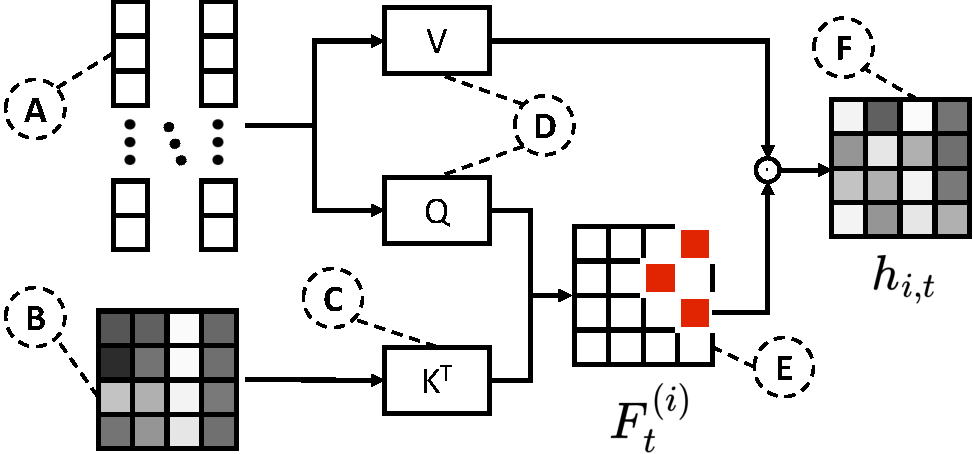
\includegraphics[width=0.75\columnwidth]{img/3-methodology/attention-diagram.pdf}
    \caption[Illustration of cross-attention mechanism]{Illustration of the cross-attention mechanism in an U-NET block: (A) the text embedding $X$; (B) the unconditioned hidden state $\hat{h}_{i,t}$;(C) the attention key $W_{k}^{(i)}\hat{h}_{i,t}$ ; (D) the attention query $W_{q}^{(i)}X$ and value $W_{v}^{(i)}X$ ; (E) the attention matrix $F_{t}^{(i)}$ (represented as red squares the activated attentions); (F) and the U-NET block output $h_{i,t}$ conditioned by the text embedding.}
    \label{fig:attention-diagram}
\end{figure}


When considering the denoising subnetwork $\epsilon_\theta$ within a Latent Diffusion Model (LDM), there are various architectural choices available. However, U-Nets \cite{UNET} have emerged as a popular option, due to their strong capabilities in image segmentation, and is the subnetwork used in Stable Diffusion (refer to Section \ref{sec:diffusion-models}). U-Nets consist of downsampling convolution blocks that preserve local context and upsampling deconvolutional blocks responsible for restoring the output to its original size \cite{DAAM}. This iterative transformation removes noise from a latent vector, ultimately producing an output image through the utilization of a Variational Autoencoder (VAE) \cite{rombach2022high}.


The denoising process operates in a lower-dimensional latent space, represented by 2D vectors denoted as $\ell_t\in \mathbb{R}^{w \times h}$ at a specific time-step $t$. In each iteration of this process, the U-NET's downsampling blocks generate a series of K intermediate states $\{ h_{i,t}^{\downarrow}\}_{i=1}^{K}$. These hidden states, with dimensions $\left \lceil \frac{w}{c^i} \right \rceil \times \left \lceil \frac{h}{c^i} \right \rceil$, gradually decrease in size as they pass through the downsampling blocks. The reduction factors $c^i$ are typically set to 1, 2, 4, and 8. Following the downsampling, the upsampling blocks scale up the downsampled hidden state $h_{K,t}^\downarrow$ to $\{ h_{i,t}^{\downarrow}\}_{i=1}^{K} \subset \mathbb{R}^{\left \lceil \frac{w}{c^i} \right \rceil \times \left \lceil \frac{h}{c^i} \right \rceil}$, effectively restoring the original dimension of the vector $\ell_t$ at the network's input. By iteratively applying this process, an approximation of the reverse diffusion process is achieved, enabling the reconstruction of an image from a noisy vector.

To incorporate textual information into the process, U-Net blocks from Stable Diffusion utilize multi-headed cross-attention layers that follow the attention mechanism proposed in the transformers architecture \cite{rombach2022high, vaswani2017attention}. This mechanism is illustrated in Figure \ref{fig:attention-diagram}. Specifically, in the case of a downsampling block, the U-Net takes a text embedding $X:= \left [ x_1; \cdots; x_{l_W}\right ] \in \mathbb{R}^{l_C \times l_W}$ consisting of $l_W$ tokens, along with the output of the fully convolutional layers of the block before conditioning, denoted as $\hat{h}_{i, t}^\downarrow$. The conditioned output $h_{i, t}^\downarrow$ of the block is then calculated as follows:


\begin{equation}
\label{eq:daam-multiscale}
\begin{gathered}
    h_{i,t}^{\downarrow} = F_t^{(i)} \left ( \hat{h}_{i, t}^{\downarrow}, X \right ) \cdot \left( W_v^{(i)\downarrow}  X \right), \\
     F_t^{(i)} \left ( \hat{h}_{i, t}^{\downarrow}, X \right ) = \text{softmax} \left( (W_q^{(i)\downarrow} \hat{h}_{i, t}^{\downarrow})  (W_k^{(i)\downarrow} X)^T / \sqrt{d} \right).
\end{gathered}
\end{equation}

In Equation \ref{eq:daam-multiscale}, the matrices $W_{k}^{(i)\downarrow}$, $W_{q}^{(i)\downarrow}$, and $W_{v}^{(i)\downarrow}$ are projection matrices with $l_{H}^{(i)}$ attention heads. These matrices transform the text embedding $X$ and $\hat{h}_{i, t}^{\downarrow}$ into vectors with dimensions $\left \lceil \frac{w}{c^i} \right \rceil \times \left \lceil \frac{h}{c^i} \right \rceil \times l_H^{(i)}$. Furthermore, the attention scores $F_{t}^{(i)\downarrow}$ have dimensions $\left \lceil \frac{w}{c^i} \right \rceil \times \left \lceil \frac{h}{c^i} \right \rceil \times l_H^{(i)} \times l_W$, which are obtained by concatenating the attention generated by each of the $l_W$ tokens.

To clarify the notation, we use $F_{t, k, h}^{(i)\downarrow}[x, y]$ to denote the attention array generated by the $k$-th token of the $h$-th multi-attention head in the $i$-th downsampling block at time $t \in \left [1, T \right]$. Similarly, in the case of upsampling blocks, we refer to their outputs as $h_{i, t}^\uparrow$ and their respective attention arrays as $F_{t, k, h}^{(i)\uparrow}[x, y]$. For brevity, when discussing an attention array that can be either from a downsampling or an upsampling block, we omit the arrow index $\downarrow$ or $\uparrow$.

In Equation \ref{eq:daam-multiscale}, it is important to note that the $\text{softmax}$ function is applied token-wise, independently for each attention head. Specifically, for each spatial coordinate $(x, y)$ and each head $h$, we have the following constraint:

\begin{equation}
    \label{eq:softmax-constraint}
    \sum_{k=1}^{l_W} F_{t, k, h}^{(i)}[x, y] = 1.
\end{equation}

This constraint ensures that, for each head and spatial point $(x, y)$, the attention is distributed among the different tokens.



To combine the attention arrays $F_{t, k, h}^{(i)} \in \mathbb{R}^{\left \lceil \frac{w}{c^i} \right \rceil \times \left \lceil \frac{h}{c^i} \right \rceil}$ from different blocks, interpolation is performed to unify them to the dimension of the original latent space $w \times h$. Due to the fully convolutional nature of the network, these arrays retain the same spatial distribution as the generated images. Therefore, scaling the attentions to different resolutions allows for their aggregation. We denote these scaled arrays as $\Tilde{F}_{t, k, h}^{(i)} \in \mathbb{R}^{w \times h}$. In the original formulation of DAAM \cite{DAAM}, the authors propose the use of bicubic interpolation for this scaling. However, in our preliminary experiments, we found that similar results in terms of IoU can be achieved using bilinear interpolation.


To create a heatmap from the scaled attention arrays, they are aggregated across all timesteps and heads using the following equation:

\begin{equation}
\label{eq:daam-summing}
    D_k^{\mathbb{R}}[x, y] := \sum_{t, i, l} \Tilde{F}_{t, k, l}^{(i) \downarrow}[x,y] + \Tilde{F}_{t, k, l}^{(i) \uparrow}[x,y].
\end{equation}

The resulting $D_k^{\mathbb{R}}$ represents a soft heat map, where higher values indicate a stronger attribution to the token $k$ (see Fig. \ref{fig:daam-example}). To convert this soft heat map into a binary mask, a threshold $\tau$ is applied relative to the maximum value of the attention map:

\begin{figure}
    \centering
    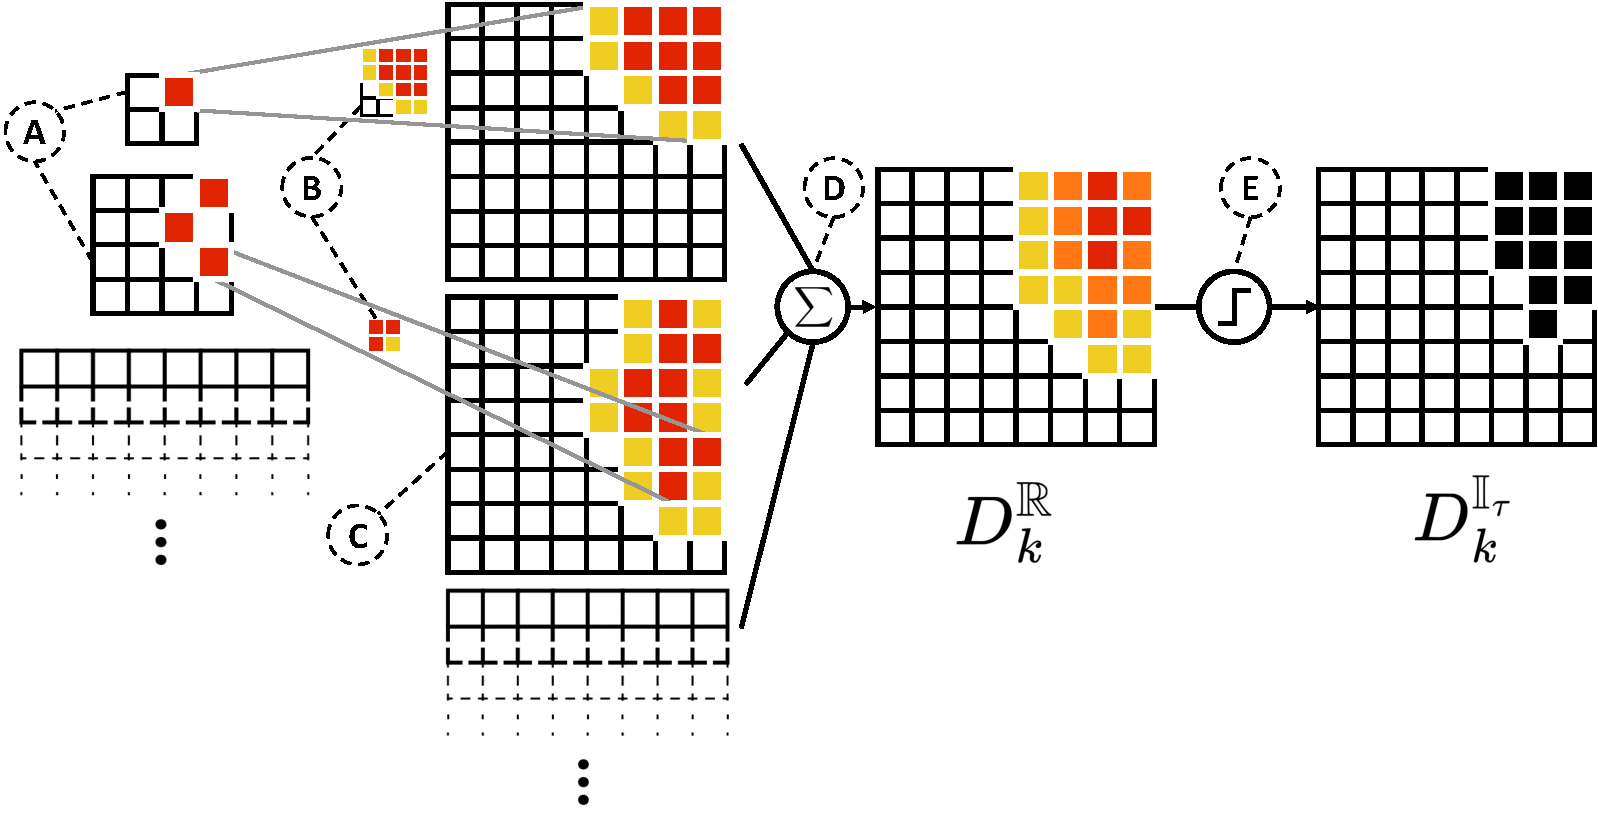
\includegraphics[width=1\columnwidth]{img/3-methodology/daam-diagram.pdf}
    \caption[Illustration of computing DAAM for some
word]{Illustration of computing DAAM for some
word: (A) the multiscale attention arrays from Eqn. \ref{eq:daam-multiscale}; (B) the bicubic interpolation  (C) resulting in expanded
maps; (D) summing the heatmaps across the layers,
as in Eqn. \ref{eq:daam-summing}; (E) and the thresholded maps. Source \cite{DAAM}.}
    \label{fig:daam}
\end{figure}


\begin{equation}
\label{eq:daam-binary}
    D_k^{\mathbb{I}_\tau}[x, y] := \mathbb{I}\left ( D_k^{\mathbb{R}}~\ge~\tau\cdot\max_{x, y}D_k^{\mathbb{R}} \right ).
\end{equation}

Here, $\mathbb{I}(\cdot)$ is the indicator function, and $\tau \in \left[0, 1 \right]$. The resulting binary mask highlights regions where the token $k$ is attributed. Figure \ref{fig:daam} provides an illustration of the DAAM construction process for a token.

DAAM serves as a powerful explainability technique for LDM, providing insights into how textual input information is synthesized and enabling the construction of semantic segmentation mechanisms. However, there are limitations to using these attention maps as ground truth for semantic segmentation tasks. For instance, binary masks depend on the threshold $\tau$, which requires further study to determine optimal values. Another limitation is that the original formulation of DAAM \cite{DAAM} does not consider generating heatmaps for tokens that are not present. This limitation prevents us from extracting masks for objects in the image, such as a tree in an urban environment, if it was not mentioned in the initial text.

Furthermore, we found that the influence area of a token does not always align with the annotation criteria of the desired semantic segmentation masks. This discrepancy arises from the semantic relationships learned by the network and the influence of the word on other parts of the scene.

These limitations make it challenging to use DAAM beyond its role as an explanation tool, especially for semantic segmentation tasks. In this work, we propose several modifications to extend the method and overcome these limitations in Sections \ref{cha:methodology-ov-daam} and \ref{cha:methodology-ov-daam-optimization}.


\section{Open Vocabulary-based DAAM}
\label{cha:methodology-ov-daam}

One of the main limitations of DAAM \cite{DAAM}, beyond its use as an explainability technique, is its restriction to generating attribution maps only for tokens present in the text prompt used to generate a sentence. This limitation becomes particularly significant when applying the method to generate semantic segmentation masks, as it would require all words to be present in the text that generated the image. In the example shown in Figure \ref{fig:daam-example}, where an image is generated with the prompt ``A car in an urban environment,'' it can be observed that besides the car, the urban scene also contains a sidewalk, a tree, and a building, for which the original method cannot generate attribution maps.

Although these tokens have not explicitly influenced the generation process, they are semantically related to elements in the generated scene. Hence, it raises the question of whether the attention they would have generated aligns with the regions corresponding to the respective objects in the image. The use of DAAM in semantic segmentation motivates the extension of the method in this regard. Furthermore, it allows for a deeper exploration of the model's internal workings, uncovering learned semantic relationships and biases.

In this section, we propose two modifications to the original formulation of 
DAAM \cite{DAAM}, which expand its capabilities by incorporating attention maps for out-of-vocabulary tokens.

First, we introduce the ``Open Vocabulary DAAM'' modification. In this approach, the original DAAM process is divided into two steps: generating the image and capturing the hidden states, followed by generating the attention matrices using an arbitrary text embedding. This modification enables the generation of heatmaps for arbitrary prompts and their tokens. However, it is important to note that the attention captured by each token is relative to the attention captured by other tokens due to the token-wise softmax operation. One limitation of this first approach is that to generate an attention heatmap for a specific word, it will be necessary to include it in a context sentence with other tokens that capture the attention of the non-interested regions.

Furthermore, we present the ``Linear Open Vocabulary DAAM'' modification. In this variant, we remove the softmax operation and directly aggregate the attention linear projections. This modification aims to explore the impact of removing the softmax operation on attention patterns and the resulting heatmaps.

We describe the procedures for generating attention maps from arbitrary sentences, addressing the challenges associated with tokens not present in the prompt.

\subsection{Open Vocabulary DAAM}
\label{sec:methodology-ov-daam-softmax}


In this subsection, we propose a modification to the construction of DAAM\cite{DAAM} to enable the evaluation of attention heatmaps for text prompts different from those used to generate the image, which guided the reverse diffusion process. To achieve this, we introduce a two-phase approach for constructing the attention maps.

In the first phase, referred to as the ``collection'' phase, a text prompt $X := [x_1; \cdots; x_{l_W}]$, referred to as the generator text embedding, is provided. An image is generated using the LDM, and during this process, the outputs of the downsampling and upsampling blocks of the U-NET prior to conditioning are saved. These outputs, denoted as $\{\hat{h}_{i,t}^{\downarrow}\}_{i=1}^{K}$ and $\{\hat{h}_{i,t}^{\uparrow}\}_{i=1}^{K}$ in equation \ref{eq:daam-multiscale}, contain spatial information about the generated image. In the original DAAM formulation \cite{DAAM}, these hidden states are used as input to the cross-attention layers of the U-NET, which incorporate the textual information and generate the attention arrays $F_{t}^{(i)}$ for constructing the DAAMs.

In the second phase, utilizing the collected hidden states $\hat{h}_{i,t}$, we construct the attention arrays based on a new text prompt. This text prompt can have different lengths and contain different tokens. Given the new text embedding $X':= [x_1; \cdots; x_{l_{W'}}] \in \mathbb{R}^{l_C \times l_{W^\prime}}$, referred to as the contextual text embedding, we generate the attribution arrays as follows:

\begin{equation}
\label{eq:daam-multiscale-ov}
\begin{gathered}
     F_{X,t}^{(i)} \left (X^\prime \right ) = \text{softmax} \left( (W_q^{(i)\downarrow} \hat{h}_{i, t}^{\downarrow})  (W_k^{(i)\downarrow} X^\prime )^T / \sqrt{d} \right).
\end{gathered}
\end{equation}

Here, $\hat{h}_{i, t}^{\downarrow}$ represents the unconditioned hidden states collected during the previous step. This computation of the attention arrays is essentially the same as the one used in the original formulation of DAAM \cite{DAAM}, utilizing the hidden states from the generator text embedding and the contextual embedding as keys in the cross-attention.
The notation $F_{X,t}^{(i)}$ is used to refer to this attention array, indicating that the hidden states $\hat{h}_{i,t}$ were generated using the text embedding $X$. Similar to Equation \ref{eq:daam-multiscale}, the $\text{softmax}$ function is applied token-wise, independently for each attention head (see the constraint in Equation \ref{eq:softmax-constraint}).

Once the new attention arrays are constructed, we can obtain the DAAMs for the text prompt $X'$ following the same methodology as in the original method \cite{DAAM}. Firstly, we rescale the spatial dimensions of the attention arrays, denoted as $\tilde{F}_{X,t}^{(i)}$, to have dimensions $w \times h \times l_{H}^{(i)} \times l_{W^\prime}$.

After constructing the rescaled attention arrays, we can generate the new heatmap based on attention by aggregating the heads from all blocks and timesteps of the process. Specifically, we have:

\begin{equation}
\label{eq:daam-summing-ov}
    D_{X,k}^{\mathbb{R}}[x, y] \left ( X^\prime \right ) := \sum_{t, i, l} \Tilde{F}_{X, t, k, l}^{(i) \downarrow}[x,y]\left ( X^\prime \right ) + \Tilde{F}_{X, t, k, l}^{(i) \uparrow}[x,y]\left ( X^\prime \right ).
\end{equation}


The entire process is illustrated in Figure \ref{fig:daam-ov-diagram}. Similar to the original version of DAAM, these modifications allow for the generation of attention heatmaps for arbitrary text prompts, providing insights into the attention patterns in the image.

  \begin{figure}
    \centering
    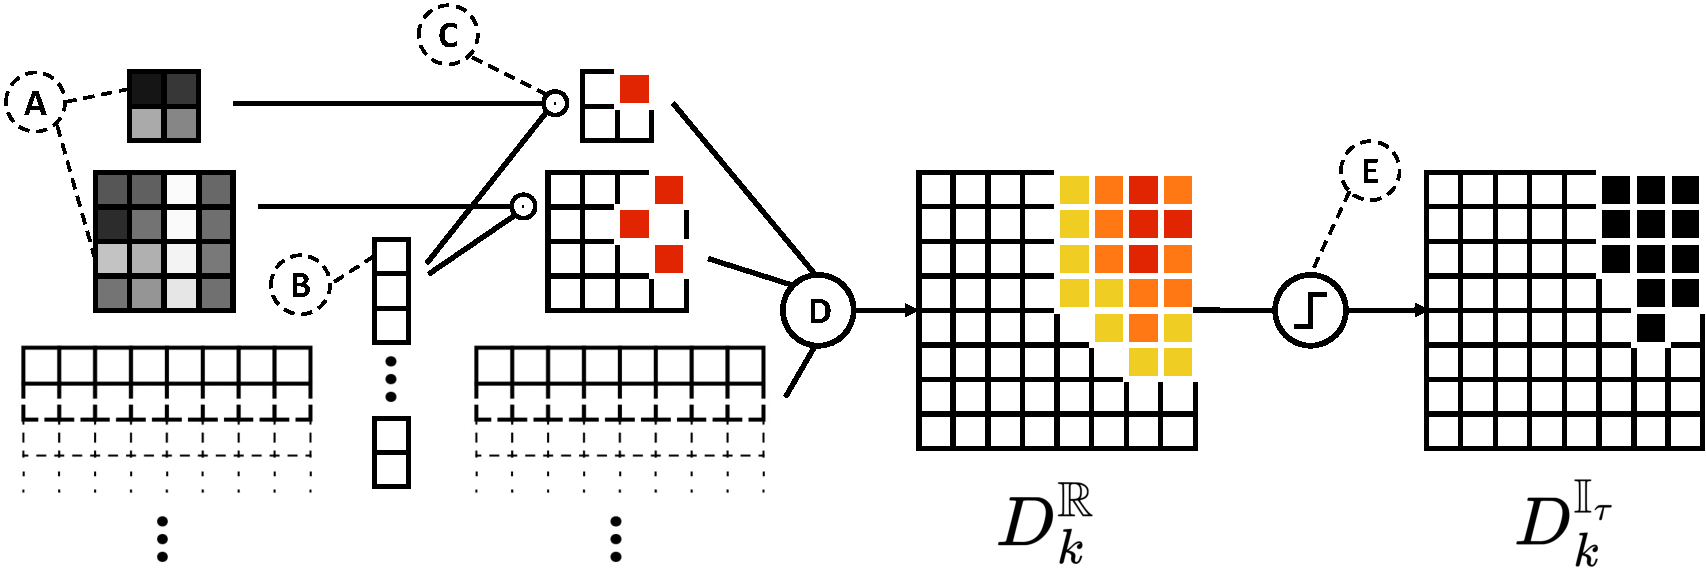
\includegraphics[width=1\columnwidth]{img/3-methodology/diagram-ov-daam.pdf}
    \caption[Illustration of computing DAAM for open
vocabulary]{Illustration of computing DAAM for open vocabulary: the hidden states $W_{q}^{(i)}\hat{h}_{i,t}^{\downarrow}$ stored during the reverse diffusion process (A); the text embedding (B); the cross-attention matrices (C) used to compute the DAAM (D); and the thresholded maps (E). Modification of figure from \cite{DAAM}.}
    \label{fig:daam-ov-diagram}
\end{figure}


Figure \ref{fig:daam-ov-example-softmax} illustrates the results of generating attention maps on the image with the prompt ``a car in an urban environment'' (see Figure \ref{fig:daam-example-image}) for the tokens ``tree,'' ``building,'' and ``sidewalk.'' As a context phrase $X'$ for extracting the attention, the phrase ``a car and a \textlangle token\textrangle\ in an urban environment'' has been used, where \textlangle token\textrangle\ represents each of the three words depicted in Figures \ref{fig:daam-ov-example-image} to \ref{fig:daam-ov-example-image-2}. The figure shows that despite not being present in the generator text prompt, the tokens are indeed related to semantically relevant areas. The attribution of the ``tree'' token is primarily focused on the tree's leaves, ``building'' is attributed to the buildings in the background, and ``sidewalk'' is attributed to the ground in the image. Therefore, it appears that the attention information successfully extends to tokens that were not present during the generation process.



\begin{figure}
\centering
  % First column
  \begin{subfigure}{0.30\columnwidth}
   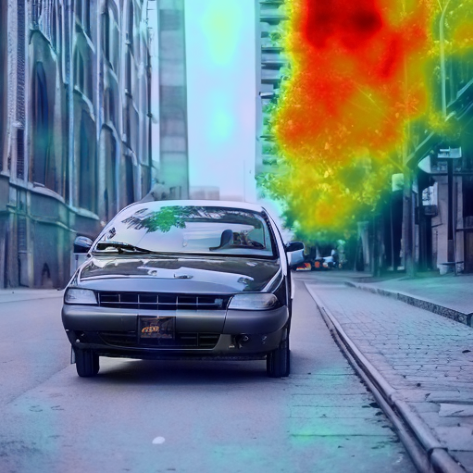
\includegraphics[width=\columnwidth]{img/3-methodology/example_ov_daam_heatmap_tree_without_special_tokens.png}
   \caption{``tree''}
   \label{fig:daam-ov-example-image}
  \end{subfigure}
  \begin{subfigure}{0.30\columnwidth}
   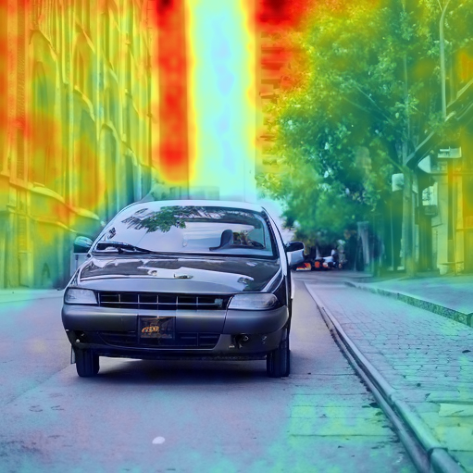
\includegraphics[width=\columnwidth]{img/3-methodology/example_ov_daam_heatmap_building_without_special_tokens.png}
   \caption{``building''}
   \label{fig:daam-ov-example-image-1}
  \end{subfigure}
  \begin{subfigure}{0.30\columnwidth}
   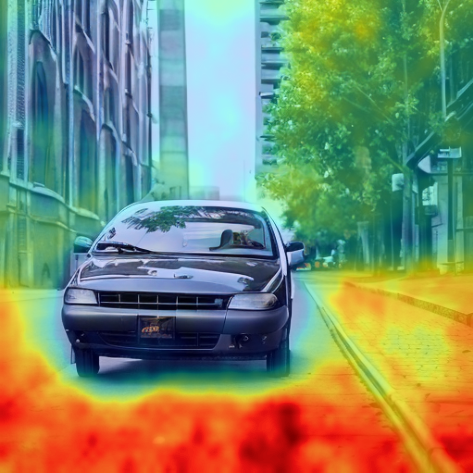
\includegraphics[width=\columnwidth]{img/3-methodology/example_ov_daam_heatmap_sidewalk_without_special_tokens.png}
   \caption{``sidewalk''}
   \label{fig:daam-ov-example-image-2}
  \end{subfigure}
  \caption[Example of Open Vocabulary DAAMs]{Example of Open Vocabulary DAAMs: An image generated with the prompt ``A car in an urban environment'' with overlaid attention maps for the tokens ``tree'' (\ref{fig:daam-ov-example-image}), ``building'' (\ref{fig:daam-ov-example-image-1}), and ``sidewalk'' (\ref{fig:daam-ov-example-image-2}). The attention maps were extracted using the contextual prompt ``A car and a \textlangle token\textrangle\ in an urban environment,'' where \textlangle token\textrangle\ represents each of the depicted words.}
  \label{fig:daam-ov-example-softmax}
  \end{figure}


This modification has significant potential as it effectively extends the attribution of different words in an image generated by an LDM to any arbitrary text prompt. However, since the attention is relative to the other tokens in the context phrase, studying the attribution of a single token becomes complex. This limitation arises when generating segmentation masks for objects in the scene. Nonetheless, it can still be valuable for other applications, such as understanding how modifications to a prompt influence image generation, enabling the construction of better prompts for LDMs.

\subsection{Linear Open Vocabulary DAAM}
\label{sec:methodology-ov-daam-linear}


One of the main limitations of the first proposed modification, the ``Open Vocabulary DAAM,'' is the requirement of defining a context phrase to extract attention maps for tokens that are not present in the prompt used to generate the image. For example, in Figure \ref{fig:daam-ov-example-softmax}, attention masks for ``tree,'' ``building,'' and ``sidewalk'' were generated using the context phrase ``A car and a \textlangle token\textrangle\ in an urban environment''. This dependence on a context phrase makes it challenging to use this extension as an explainability method for understanding the relation of standalone words in the image, as well as for generating attention masks for individual objects in synthetic images. The attribution generated by this method strongly relies on how the contextual phrase is constructed. Thus, there is a need to find a way to extract attention without considering the attention of other tokens.

After conducting several preliminary experiments to study the role of the softmax function in the attribution of different tokens in the phrase, it was found that aggregating the attentions of a single token without applying $\text{softmax}$ still resulted in attention heatmaps focused on the same areas as when using a tailored context phrase. Therefore, the second proposed variation, called ``Linear Open Vocabulary DAAM,'' is a modification of the previous method without the application of $\text{softmax}$.


To generate a Linear DAAM, the first step is to perform a collection phase. This is done by generating an image with a text prompt $X$ and capturing the hidden states $\hat{h}_{i,t}$. This collection phase is identical to the one proposed in the previous extension (see section \ref{sec:methodology-ov-daam-softmax}).


Once the hidden states have been captured, we proceed to compute the attention of an individual token without applying the softmax function, as defined in Equation \ref{eq:daam-multiscale-ov}. Specifically, for a given token embedding $x$ for which we aim to generate an attribution map, the attention is calculated as:

\begin{equation}
\label{eq:daam-multiscale-ov-linear}
\begin{gathered}
     L_{X,t}^{(i)} \left (x \right ) = (W_q^{(i)\downarrow} \hat{h}_{i, t}^{\downarrow})  (W_k^{(i)\downarrow} x )^T \, .
\end{gathered}
\end{equation}

In this context, the attention array $L_{X,t}^{(i)}\in \mathbb{R}^{\left \lceil \frac{w}{c^i} \right \rceil \times \left \lceil \frac{h}{c^i} \right \rceil \times l_{H}^{(i)}}$ corresponds to the result of computing the dot product between the query projection $W_q^{(i)\downarrow} \hat{h}_{i, t}^{\downarrow}$ and the key projection $W_k^{(i)\downarrow} x$. This computation enables us to capture the token's relevance within the image, without the incorporation of the softmax normalization utilized in Equation \ref{eq:daam-multiscale-ov}.
Subsequently, the attention arrays are rescaled to dimensions $w \times h \times l_{H}^{(i)}$, denoted as $\tilde{L}_{X,t}^{(i)}$, to facilitate their aggregation. Finally, all the attention arrays are combined into a unified heatmap by summing them together.

\begin{equation}
\label{eq:daam-summing-ov-linear}
    {LD}_{X}^{\mathbb{R}}[x, y] := \sum_{t, i, l} \Tilde{L}_{X, t, l}^{(i) \downarrow}[x,y] + \Tilde{L}_{X, t, l}^{(i) \uparrow}[x,y].
\end{equation}


\begin{figure}
\centering
  % Second column
  \begin{subfigure}{0.30\columnwidth}
   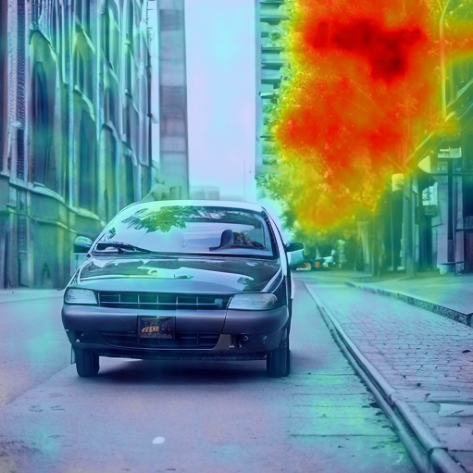
\includegraphics[width=\columnwidth]{img/3-methodology/example_ov_daam_heatmap_tree_without_context.png}
   \caption{``tree''}
   \label{fig:daam-ov-example-image-3}
  \end{subfigure}
  \begin{subfigure}{0.30\columnwidth}
   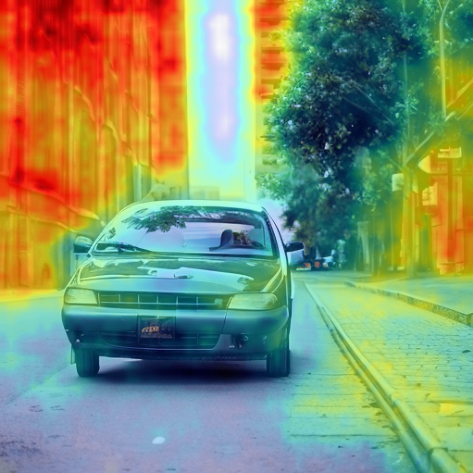
\includegraphics[width=\columnwidth]{img/3-methodology/example_ov_daam_heatmap_building_without_context.png}
   \caption{``building''}
   \label{fig:daam-ov-example-image-4}
  \end{subfigure}
  \begin{subfigure}{0.30\columnwidth}
   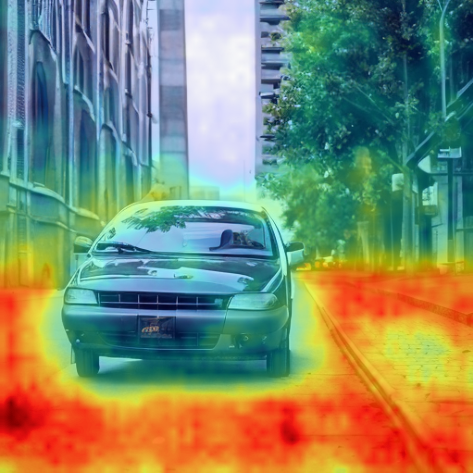
\includegraphics[width=\columnwidth]{img/3-methodology/example_ov_daam_heatmap_sidewalk_without_context.png}
   \caption{``sidewalk''}
   \label{fig:daam-ov-example-image-5}
  \end{subfigure}
  \caption[Example of Linear Open Vocabulary DAAMs]{Example of Linear Open Vocabulary DAAMs: An image generated
with the prompt ``A car in an urban environment'' with overlaid linear attention maps for the
tokens ``tree'' (\ref{fig:daam-ov-example-image-3}), ``building'' (\ref{fig:daam-ov-example-image-4}), and ``sidewalk'' (\ref{fig:daam-ov-example-image-5}).}
  \label{fig:daam-ov-example-linear}
  \end{figure}

In Figure \ref{fig:daam-ov-example-linear}, the results of three linear attention maps, denoted as ${LD}_{X}^{\mathbb{R}}$ in eq. \ref{eq:daam-summing-ov-linear}, are presented for the tokens ``tree,'' ``building,'' and ``sidewalk'' on the example image generated with the text prompt ``A car in an urban environment.'' The example demonstrates how these heatmaps generate attention in the same regions as their $\text{softmax}$ counterparts, without the need for a context phrase that interferes with their attention. This characteristic enhances their utility as an explainability method, simplifying the examination of biases acquired by a model or the generation of semantic segmentation masks based on a single word.

However, despite the potential of this method as an explainability technique for LDMs, it is still limited as a standalone approach for extracting ground truth in semantic segmentation tasks. A key limitation shared with the original DAAM approach \cite{DAAM} is that the regions attributed to a word may not align with the semantic segmentation mask assigned to the class represented by that word. For instance, in Figure \ref{fig:daam-ov-example-image-5}, it is evident that the attribution of the word ``sidewalk'' also extends attention to the road section, which is typically labeled as a distinct class in urban scene segmentation tasks. In other cases, the word may generate attention in other areas due to different learned semantic relationships within the network. To rigorously investigate this issue, an optimization approach for searching the text embedding that maximizes the Intersection over Union (IoU) with the target region is proposed in Section \ref{cha:methodology-ov-daam-optimization}.


\section{Prompt optimization via DAAM}
\label{cha:methodology-ov-daam-optimization}


The proposed extensions of DAAM for open vocabulary usage provide increased flexibility as an explainability tool. They allow us to highlight the semantic relationships learned by a Latent Diffusion Model (LDM), such as Stable Diffusion, by examining the influence of words on its internal attentions. However, initial tests showed that the attribution maps extracted for object nouns in generated images often do not align with the corresponding ground truth semantic segmentation masks. Although these maps demonstrate semantic coherence, they also include unwanted regions, which presents challenges for their application beyond explainability.

For instance, the attribution map for the word ``building'' (Figure \ref{fig:daam-ov-example-image-4}) extended its influence to the sidewalk, likely due to their semantic association within the urban context. In another case (Figure \ref{fig:daam-ov-example-image-5}), the ``sidewalk'' map also encompassed the road area, deviating from the desired segmentation. Such irregularities impede the effective use of attention maps in semantic segmentation tasks.

To address these limitations, we propose approaching the problem as a minimization problem solved through gradient descent on the extension of DAAM for Open Vocabulary proposed in this work (Fig. \ref{fig:daam-optimization-diagram} illustrates this process). We will focus on formulating the method in its simplest variant: the search for a single token, $x$, that maximizes a specific region based on its Linear DAAM.


\begin{figure}
    \centering
    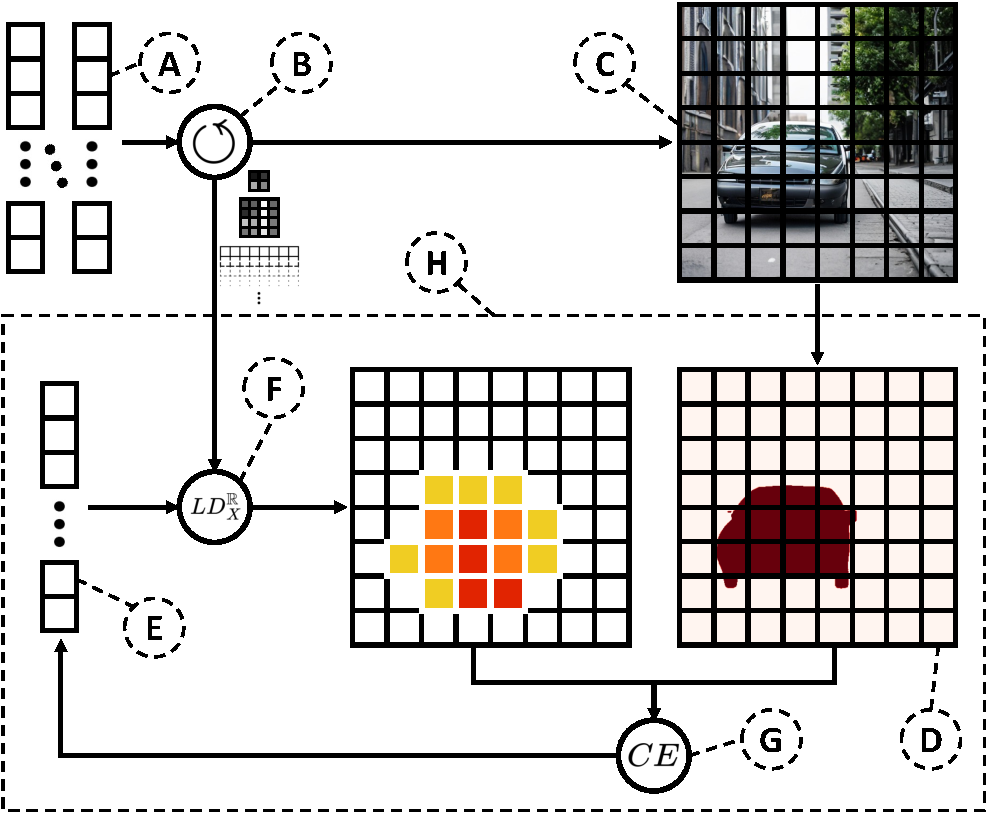
\includegraphics[width=0.8\columnwidth]{img/3-methodology/optimization-diagram.pdf}
    \caption[Prompt Optimization Process Diagram]{Prompt Optimization Process Diagram. The diagram illustrates the following steps: (A) Input of a text embedding $X$ into a LDM (B), resulting in the generation of a synthetic image (C). (D) The target mask is annotated. A token embedding $x$ (E) is utilized to generate the Open Vocabulary DAAM (F). The error between the target mask and the attention heatmap is calculated, and gradients are backpropagated (G) and $x$ is updated. (H) This process is repeated within an optimization loop.}
    \label{fig:daam-optimization-diagram}
\end{figure}

A Linear DAAM, denoted as ${LD}^\mathbb{R}_X$, can be understood as a function that takes a token embedding, $x\in \mathbb{R}^{l_C}$ and a set of hidden states, ${LD}^\mathbb{R} ( X^\prime; \hat{h}_{1, 1}^\downarrow, \cdots, \hat{h}_{T, K}^\uparrow )$, and generates an attention map. In this optimization, we keep the hidden states fixed and consider the DAAM solely as a function of $x$, indicated by the subscript $X$ to represent the text embedding that generated these states. In other words, ${LD}^\mathbb{R}_X\left ( \cdot \right):\mathbb{R}^{l_C} \to \mathbb{R}^{w \times h}$. To formulate the optimization problem, we introduce a binary mask, $G_X \in \mathbb{R}^{w \times h}$, representing the ground truth of the target influential area. Our objective is to minimize a cost function $C$, which should be differentiable, in charge of measure the divergence between the output of the Linear DAAM and the ground truth $G_X$:

\begin{equation}
\label{eq:objective-optimization}
    \hat{x} = \arg\min_{x} C \left ( {LD}_X^{\mathbb{R}}\left ( x \right ), G_X \right ) .
\end{equation}

This objective function (Eq. \ref{eq:objective-optimization}) is differentiable with respect to $x$, as ${LD}_X^{\mathbb{R}}$ is the sum of linear projections of the input token (Eq. \ref{eq:daam-multiscale-ov-linear}) and spatial interpolations of these projections (Eq. \ref{eq:daam-summing-ov-linear}). Therefore, we can optimize the objective function using gradient descent. Figure \ref{fig:daam-optimization-diagram} illustrates this iterative optimization process, where the token embedding is updated based on the gradients of the objective function.

We found that the cross-entropy loss between the soft heatmap and the ground truth worked effectively for the optimization. The cross-entropy loss is defined as:

% Nota para Roberto sobre notacion: 
% Se que la letra "x" se utiliza tanto para indicar el token siendo maximizado
% como la coordenada espacial x (de las x,y). Es notación heredada del paper
% de DAAM, la utilizan de forma repetida. La habría cambiado en esta memoria,
% pero es que no me quedan letras y no me apetece 
% meter letras griegas y cambiar la notacion del paper original XD
% Pasa lo mismo con la letra h, que se usa para la dimension w x h
% y como variable en los sumatorios que indica suma sobre multihead attentions.

\begin{equation}
\label{eq:cross-entropy}
    CE_{loss} \left ({LD}_X^{\mathbb{R}}, G_X \right ) = - \sum_{x, y} G_X [x, y]\cdot \log \left ( {LD}^{\mathbb{R}}_X [x, y] \right ) .
\end{equation}

To compute the cross-entropy loss, the heatmap needs to be normalized in the range of $[0, 1]$. Since the linear DAAM is a sum of linear projections and is not inherently normalized like softmax-based heatmaps. We employed a linear scaling, also known as min-max scaling, to resize the heatmap values to the desired range of $[0, 1]$. This normalization effectively scaled the heatmap values, ensuring consistent visualization of the heatmaps throughout the optimization process. For clarity, the normalization step has not been included in the notation of Equation \ref{eq:cross-entropy}.

\begin{figure}
\centering
  \begin{subfigure}{0.30\columnwidth}
   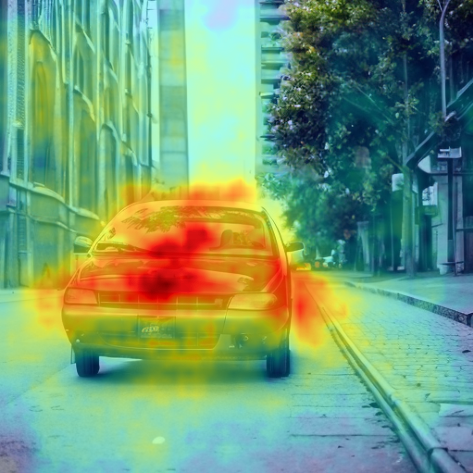
\includegraphics[width=\columnwidth]{img/3-methodology/initial_mask.png}
   \caption{Initial heatmap}
   \label{fig:optimization-initial-mask}
  \end{subfigure}
  \begin{subfigure}{0.30\columnwidth}
   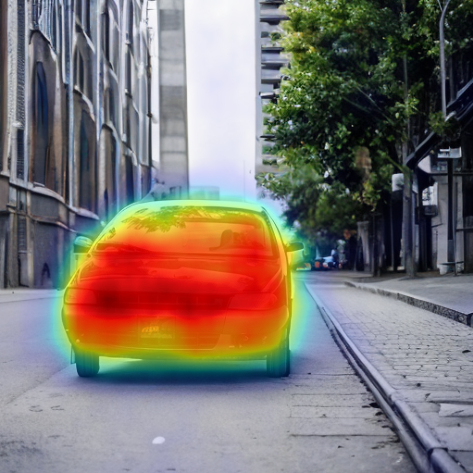
\includegraphics[width=\columnwidth]{img/3-methodology/optimized_mask.png}
   \caption{Optimized heatmap}
   \label{fig:optimization-optimized-mask}
  \end{subfigure}
  \begin{subfigure}{0.30\columnwidth}
   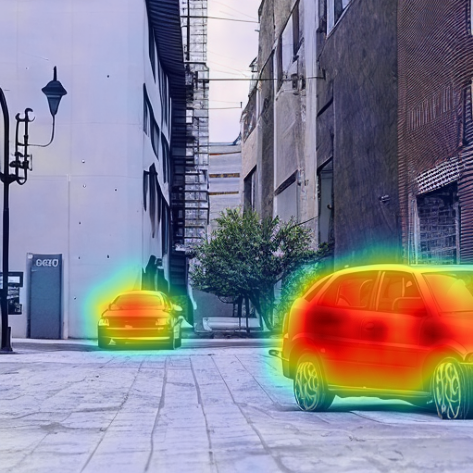
\includegraphics[width=\columnwidth]{img/3-methodology/extrapolated_mask.png}
   \caption{Transferred heatmap}
   \label{fig:optimization-extrapolated-mask}
  \end{subfigure}
  \caption[Example of Optimization via DAAM]{Example of Optimization via DAAM. The figure showcases the optimization process applied to the example image (Fig \ref{fig:daam-example-image}). It includes the initial Linear DAAM of the token ``car'' overlaid on the image (Fig. \ref{fig:optimization-initial-mask}), the optimized heatmap generated by $\hat{x}$ (Fig. \ref{fig:optimization-optimized-mask}), and the Linear DAAM of $\hat{x}$ on a different image (Fig. \ref{fig:optimization-extrapolated-mask}).}
  \label{fig:example-optimization}
  \end{figure}


Figure \ref{fig:example-optimization} visually presents the optimization results conducted on the example image discussed throughout this chapter (Fig. \ref{fig:daam-example-image}). 
In Fig. \ref{fig:optimization-initial-mask}, we observe the Linear DAAM generated for the token ``car.'' A comparison with the DAAM generated using the original non-linear method (Fig. \ref{fig:daam-example-image-3}) reveals notable differences in behavior. While the resulting mask maintains its focus on the car, it exhibits a broader influence that extends beyond the immediate region. This is because the absence of softmax normalization between tokens in a text embedding allows the attention to encompass surrounding background areas.

To tackle this issue, we utilize ``car'' as the initial token $x$ for the optimization process. The resulting heatmap generated by $\hat{x}$ after optimization is depicted in Figure \ref{fig:optimization-optimized-mask}. It can be observed that the resulting area more precisely delineates the region surrounding the car, without attracting attention from the urban environment.

To assess the semantic information encapsulated within $\hat{x}$ and its generalizability, we evaluate its performance on a different image generated by the LDM. As shown in Figure \ref{fig:optimization-extrapolated-mask}, we observe a scene featuring two cars on a street. Notably, the optimized vector effectively generates attention around both car instances, indicating the transferability of learned semantic knowledge to influence attentions in diverse image contexts.

Furthermore, this approach is also valid for optimizing Open Vocabulary DAAMs, in which we would need to jointly optimize a text embedding $X^\prime = [x_1, ...; x_{l_{W^\prime}}]$ with a segmentation mask for each token in the phrase. In this case $D^\mathbb{R}_X\left ( \cdot \right):\mathbb{R}^{l_C \times l_{W^\prime}} \to \mathbb{R}^{w \times h \times l_{W^\prime}}$. 

In the general case, where $X^\prime$ is optimized across multiple images generated with text prompts $\{X_j\}_{j=1}^N$, where the length of the tokens $X_j$ can vary, the objective function is defined as follows:

\begin{equation}
\label{eq:general-objective}
    \hat{X^\prime} = \arg\min_{X^\prime} \sum_{j=1}^N \sum_{k=1}^{l_{W^\prime}} C \left ( D_{ X_j, k}^{\mathbb{R}}\left ( X^\prime \right ), G_{X_j, k} \right ) .
\end{equation}

Where for practical experiments we use as loss $C$ the cross entropy $CE_{loss}$.
This objective function (Eq. \ref{eq:general-objective}) shares similarities with the loss function employed in training a semantic segmentation model. However, unlike traditional training with images, we utilize the attentions generated during their generation in the LDM (indexed by $j$). Instead of working with multiple semantic classes as the output objective, we focus on optimizing the activations of multiple tokens (indexed by $k$). Moreover, instead of updating the weights of the model, our optimization process revolves around refining the input text embedding ($X^\prime \in \mathbb{R}^{l_C \times l_{W^\prime}}$) . It is important to emphasize that, similar to a semantic segmentation model, we utilize binary masks as ground truth for each image and class/token in the training dataset ($G_{X_j}, k$). Figure \ref{fig:daam-general-optimization-diagram} illustrates the procedure proposed to optimize this function.
%Experiments conducted (Sec. \ref{sec:experiment-optimization}) indicate that only 1 or 2 annotated images for class are sufficient to optimize the text embedding for a simple dataset.

In the following chapter, we conduct practical experiments aimed at analyzing the potential of prompt optimization via DAAM method in generating accurate segmentation masks. These experiments explore the effectiveness of the optimization process by assessing the quality and alignment of the generated masks in comparison to the ground truth annotations. Moreover, we investigate the generalization capabilities of the optimized text embeddings across a diverse range of images generated by the LDM.

\begin{figure}
    \centering
    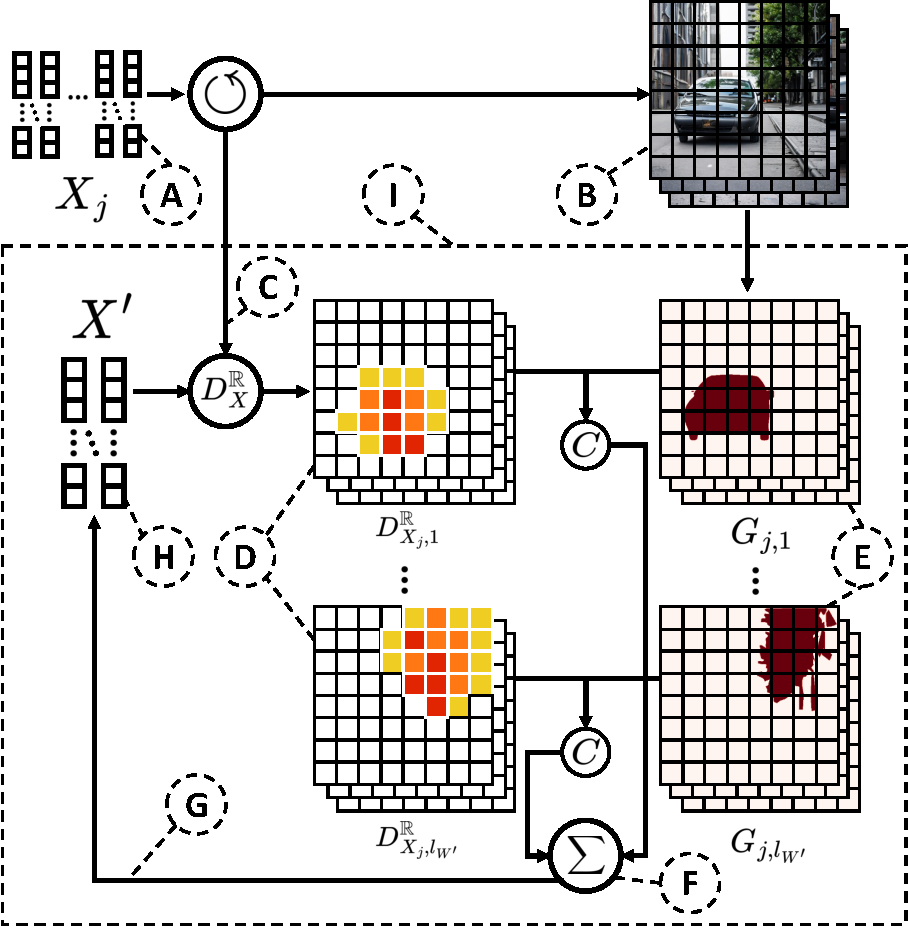
\includegraphics[width=0.8\columnwidth]{img/3-methodology/general-optimization.pdf}
    \caption[Prompt Optimization Diagram. General case.]{Optimization process of DAAM in the general case. The diagram illustrates the following steps: (A) Inputting the set of text embeddings $X_j$ into a LDM, resulting in the generation of synthetic images (B). The attentions generated by the LDM are fixed in the DAAM function (C). DAAM generates heatmaps (D) corresponding to the target masks (E), which are used to compute the loss for each image and token (F). The gradients of the loss are propagated (G) and employed to update the text embedding $X^\prime$ (H). This iterative process occurs within an optimization loop (I).}
    \label{fig:daam-general-optimization-diagram}
\end{figure}
              % incluir capítulo de evaluacion/evaluation
%%%%%%%%%%%% DISEÑO Y DESARROLLO / DESIGN & IMPLEMENTATION CHAPTER %%%%%%%%%%%%%%%%%%%%%%%%%%%%%%%%%%%%%%%%%%%
\chapter{Experiments and Results}
\label{cha:experiments}

This chapter presents a series of practical experiments aimed at exploring the potential of utilizing DAAM and the proposed extensions for object segmentation in synthetically generated images, particularly focusing on urban scenes. To conduct these experiments, a synthetic dataset was created using Stable Diffusion as the foundational model (Sec. \ref{sec:experiment-framework}). The experiments are organized into three sections, mirroring the structure of the proposed methods proposed in Chapter \ref{cha:methodology}, in order to assess the impact of each modification.

The first section, \ref{sec:experiment-daam}, evaluates the masks generated by DAAM in its original formulation \cite{DAAM} to establish a baseline for comparing the proposed modifications. Next, in section \ref{sec:experiment-daam-ov}, we measure the effects of linearizing the attention maps using Linear DAAMs (Sec. \ref{cha:methodology-ov-daam}). In section \ref{sec:experiment-optimization}, we optimize text prompts for each class in the dataset and repeat the evaluation. Finally, in Section \ref{sec:experiment-summary}, we provide a summary of the experiment and a comparison of the results.

The goal of these experiments is to analyze the limitations and potential benefits of utilizing internally generated attentions from an LDM within a simplified urban scene scenario. Additionally, we aim to identify possible directions for future research, expanding the application of DAAM beyond its initial framework.

\section{Experiment framework}
\label{sec:experiment-framework}

This section overviews the experiment framework, including the architecture used and the details of the generated dataset.

To conduct the experiments, a synthetic dataset of simple urban scene scenarios was created. The dataset was intentionally designed to emphasize simplicity, with each image featuring a single primary object class. Four commonly encountered classes \cite{Cityscapes} in urban scene semantic segmentation tasks were chosen: ``car,'' ``person,'' ``traffic light,'' and ``rider''.

The images were generated using the Stable Diffusion (2-base) architecture, which was also employed in the original DAAM paper \cite{DAAM}. However, the proposed methods and implementation are compatible with other versions of Stable Diffusion \cite{rombach2022high}. Initial tests conducted with other versions have yielded similar results.

 A dataset consisting of 200 images was created, with 50 images per class. The text prompt ``A \textlangle token\textrangle\ in an urban environment'' was utilized to generate the images, where the token corresponds to each class name. In order to generate diverse images with the same text prompt, the random seed used to generate the initial noisy latent vector was changed for each image. For more detailed information about the dataset and to access the images, please refer to Appendix \ref{chap:appendix-text-dataset}.
 
The LDM noise modeling process employs the PNDM scheduler \cite{liu2022pseudo}, which utilizes a multi-step Runge-Kutta method to model the diffusion process as an ODE and accelerate the convergence of the diffusion process. The reverse diffusion model uses 30 timesteps to generate the images. To ensure reproducibility, the random seeds used in the process were stored, allowing for the replication of the diffusion process and generation of the same images and internal attentions.



\begin{figure}
\centering
  % First column
  \begin{subfigure}{0.24\columnwidth}
   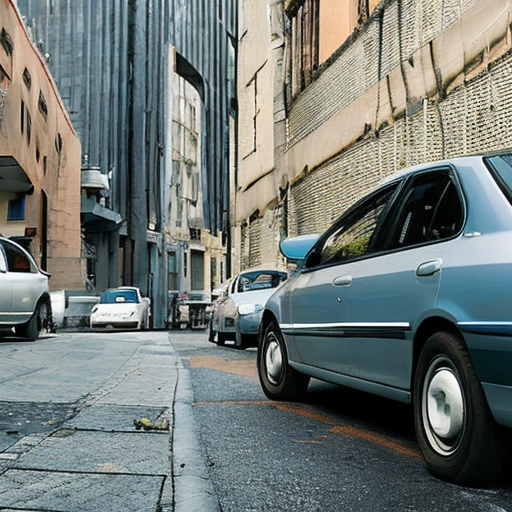
\includegraphics[width=\columnwidth]{img/4-experiments/dataset_example_car.png}
   \caption{Car}
   \label{subfig:dataset-example-car}
  \end{subfigure}
  \begin{subfigure}{0.24\columnwidth}
   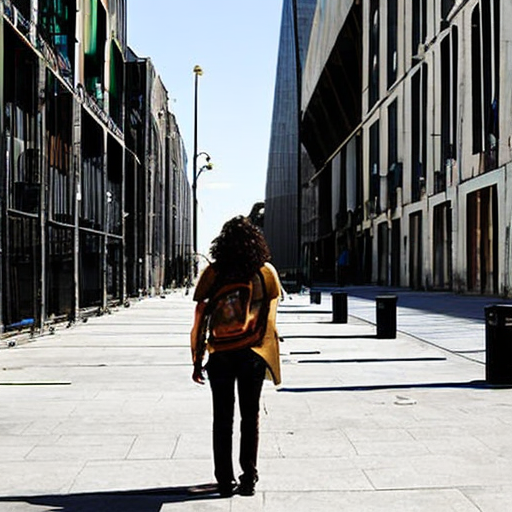
\includegraphics[width=\columnwidth]{img/4-experiments/dataset_example_person.png}
   \caption{Person}
   \label{subfig:dataset-example-person}
  \end{subfigure}
  \begin{subfigure}{0.24\columnwidth}
   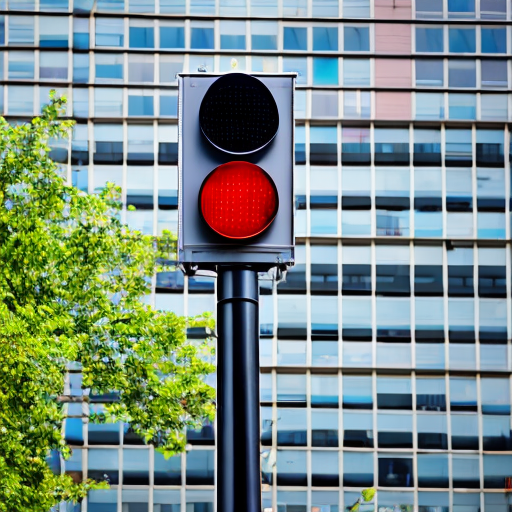
\includegraphics[width=\columnwidth]{img/4-experiments/dataset_example_traffic light.png}
   \caption{Traffic Light}
   \label{subfig:dataset-example-traffic}
  \end{subfigure}
  \begin{subfigure}{0.24\columnwidth}
   \includegraphics[width=\columnwidth]{img/4-experiments/dataset_example_rider.png}
   \caption{Rider}
   \label{subfig:dataset-example-rider}
  \end{subfigure}
  \par\bigskip
  \begin{subfigure}{0.24\columnwidth}
   \includegraphics[width=\columnwidth]{img/4-experiments/example_mask_car.png}
   \caption{Car mask}
   \label{subfig:dataset-example-car-mask}
  \end{subfigure}
  \begin{subfigure}{0.24\columnwidth}
   \includegraphics[width=\columnwidth]{img/4-experiments/example_mask_person.png}
   \caption{Person mask}
   \label{subfig:dataset-example-person-mask}
  \end{subfigure}
  \begin{subfigure}{0.24\columnwidth}
   \includegraphics[width=\columnwidth]{img/4-experiments/example_mask_traffic light.png}
   \caption{Traffic light mask}
   \label{subfig:dataset-example-traffic-mask}
  \end{subfigure}
    \begin{subfigure}{0.24\columnwidth}
   \includegraphics[width=\columnwidth]{img/4-experiments/example_mask_rider.png}
   \caption{Rider mask}
   \label{subfig:dataset-example-rider-mask}
  \end{subfigure}
  \caption[Synthetic dataset examples]{Visual examples of images and corresponding segmentation masks in the dataset. The first row showcases four distinct scenes, each representing one of the classes: ``car'', ``person'', ``traffic light'', and ``rider''. In the second row, the same images are presented with their respective ground truths overlayed.}
  \label{fig:dataset-examples}
  \end{figure}
  
Figure \ref{fig:dataset-examples} showcases an example image for each of the four classes in the dataset (Figs. \ref{subfig:dataset-example-car} to \ref{subfig:dataset-example-rider}). The images illustrate the simplicity of the scenes, with a clear focus on a single primary object from each class.

Ground truth annotations were created for each of the 200 images based on their corresponding primary class, following the standards used in Cityscapes \cite{Cityscapes}. The SAM (Segment Anything Model) \cite{SAM} was employed to generate accurate segmentation masks, with manual supervision to ensure precise annotations. These segmentation masks serve as the reference for measuring the Intersection over Union (IoU) between the binary heatmaps generated by DAAM and its proposed extensions.

The latent space dimensions of Stable Diffusion 2-base (referred to as $w \times h$ in Chapter \ref{cha:methodology}), and therefore the dimensions of the generated attention maps, are 64 x 64. However, the images are generated at a resolution of 512 x 512, due to the VAE final step \cite{rombach2022high}. To measure the IoU, the heatmaps are rescaled using bicubic interpolation to match the size of the images.


Examples of the binary masks can be seen in Figs. \ref{subfig:dataset-example-car-mask} to \ref{subfig:dataset-example-rider-mask}. Notably, for the traffic light class (\ref{subfig:dataset-example-traffic-mask}), the post is excluded, as it is typically labeled as class ``pole'' in urban scene segmentation datasets. Similarly, the rider class includes only the person riding the motorcycle, without including the motorcycle itself (\ref{subfig:dataset-example-rider-mask}).




\section{DAAM baseline}
\label{sec:experiment-daam}

\begin{figure}
\centering
  % First column
  \begin{subfigure}{0.24\columnwidth}
   \includegraphics[width=\columnwidth]{img/4-experiments/dataset_example_daam_heatmap_car.png}
   \caption{Car}
   \label{subfig:dataset-example-car-daam}
  \end{subfigure}
  \begin{subfigure}{0.24\columnwidth}
   \includegraphics[width=\columnwidth]{img/4-experiments/dataset_example_daam_heatmap_person.png}
   \caption{Person}
   \label{subfig:dataset-example-person-daam}
  \end{subfigure}
  \begin{subfigure}{0.24\columnwidth}
   \includegraphics[width=\columnwidth]{img/4-experiments/dataset_example_daam_heatmap_traffic light.png}
   \caption{Traffic light}
   \label{subfig:dataset-example-traffic-daam}
  \end{subfigure}
  \begin{subfigure}{0.24\columnwidth}
   \includegraphics[width=\columnwidth]{img/4-experiments/dataset_example_daam_heatmap_rider.png}
   \caption{Rider}
   \label{subfig:dataset-example-rider-daam}
  \end{subfigure}
  \caption[Examples of DAAM-generated soft heatmaps]{Examples of DAAM-generated soft heatmaps. Each subfigure displays an image for each class with the overlayed soft heatmap generated using DAAM.}
  \label{fig:dataset-examples-daam}
  \end{figure}

In this initial experiment, we evaluate the masks generated by the original DAAM method \cite{DAAM}. These findings establish a baseline for understanding the performance of DAAM's attention in semantic segmentation tasks and identifying the key challenges that arise when using this explainability technique in such contexts.

To evaluate the masks, we generated soft heatmaps, $D^{\mathbb{R}}_k$, following Eq. \ref{eq:daam-summing}, using the original implementation of DAAM. The token corresponding to the class name was extracted from the text prompt ``A \textlangle token\textrangle\ in an urban environment'' for each class, except for the ``traffic light'' class, which consisted of two tokens. To prevent attention from being dispersed throughout the entire scene due to the semantic association with the word ``traffic,'' we specifically considered the token ``light'' for this class.

Figure \ref{fig:dataset-examples-daam} displays the soft heatmaps for each example image of the four classes. We observe distinct issues in each class, which can be explained from a semantic perspective of the generated attention:

\begin{itemize}
\item In the example of the ``car'' class (Fig. \ref{subfig:dataset-example-car-daam}), the attention attributed to the word ``car'' correctly focuses on the cars. However, the attention within these cars is irregular, and in this specific example, there is minimal attention given to the cars in the background of the scene.
\item For the ``person'' class (Fig. \ref{subfig:dataset-example-person-daam}), the attention is dispersed throughout the image, as the semantic relationship learned by the network for the word ``person'' influences the entire scene.
\item In the ``traffic light'' class (Fig. \ref{subfig:dataset-example-traffic-daam}), where we considered the attention generated by the word ``light,'' the attention correctly focuses on the red light of the traffic signal (see Fig. \ref{subfig:dataset-example-traffic}). However, the segmentation does not cover the entire expected area according to the annotation criteria (\ref{subfig:dataset-example-traffic-mask}).
\item For the ``rider'' class (Fig. \ref{subfig:dataset-example-rider-daam}), the attention is primarily concentrated on the motorcycle. This could be interpreted as the network learning that the presence of a motorcycle gives semantic meaning to the concept rider. However, our goal is to obtain a mask that specifically segments the person riding the motorcycle.
\end{itemize}

\begin{figure}
    \centering
    \includegraphics[width=1\columnwidth]{img/4-experiments/daam-threshold-iou-experiment-min-max.pdf}
    \caption[Comparison of mIoU per class using DAAM]{Comparison of mean Intersection over Union (mIoU) for each class at different threshold values. The graph illustrates the mIoU values for the ``car,'' ``light,'' ``person,'' and ``rider'' classes, along with the 5th and 95th percentile values. The curves demonstrate distinct profiles for each class, highlighting the varying performance of DAAM in segmenting different object classes.}
    \label{fig:miou-class-curves}
\end{figure}


To assess the performance in terms of mIoU, we employed a fixed threshold to binarize the heatmaps (as per Eq. \ref{eq:daam-binary}). Considering that mIoU is dependent on the threshold, we varied it from 0 to 1 to examine the curves' behavior. The results of the experiment are shown in Figure \ref{fig:miou-class-curves}, revealing four distinct patterns for each class. The figure showcases the mIoU (per-pixel) for each class and includes the 5th and 95th percentile mIoU values for individual class examples. It is noteworthy that the behavior of mIoU across different thresholds remains consistent within each class. The curves' profiles can be explained by the challenges illustrated in the previous examples, which are prevalent throughout the dataset:

\begin{itemize}
\item The ``car'' class is segmented correctly, reaching a maximun mIoU of 82.5.
\item The ``light'' class achieves an mIoU of 71.1, as the attention generated only relates to the light part of the traffic light.
\item The ``person'' class reaches an mIoU of 36.2, as the attention is centered on the persons' silhouettes but generates dispersed attention throughout the scenes.
\item The ``rider'' class has a maximum IoU of 31.0 because the network's concept aligns with the object ``motorcycle'' rather than the rider.
\end{itemize}

These results underscore the limitations of utilizing DAAM as a direct means of extracting ground truth, even in a straightforward scenario. The challenge lies in effectively controlling the attention's focus, which is constrained by the choice of words in the prompt used to generate the image. In the subsequent experiments, we examine this same scenario using the proposed modifications of the method, aiming to extend its applicability beyond its original purpose of explainability.


\section{Linear Open Vocabulary DAAM}
\label{sec:experiment-daam-ov}


\begin{figure}
\centering
  % First column
  \begin{subfigure}{0.24\columnwidth}
   \includegraphics[width=\columnwidth]{img/4-experiments/example-linear-daam-overlay-car.png}
   \caption{Car}
   \label{subfig:dataset-example-car-daam-linear}
  \end{subfigure}
  \begin{subfigure}{0.24\columnwidth}
   \includegraphics[width=\columnwidth]{img/4-experiments/example-linear-daam-overlay-person.png}
   \caption{Person}
   \label{subfig:dataset-example-person-daam-linear}
  \end{subfigure}
  \begin{subfigure}{0.24\columnwidth}
   \includegraphics[width=\columnwidth]{img/4-experiments/example-linear-daam-overlay-traffic light.png}
   \caption{Traffic light}
   \label{subfig:dataset-example-traffic-daam-linear}
  \end{subfigure}
  \begin{subfigure}{0.24\columnwidth}
   \includegraphics[width=\columnwidth]{img/4-experiments/example-linear-daam-overlay-rider.png}
   \caption{Rider}
   \label{subfig:dataset-example-rider-daam-linear}
  \end{subfigure}
  \caption[Examples of Linear DAAM-generated soft heatmaps]{Examples of Linear DAAM-generated soft heatmaps. Each subfigure displays an image for each class with the overlayed soft heatmap generated using Linear DAAM.}
  \label{fig:dataset-examples-daam-linear}
  \end{figure}


\begin{figure}
    \centering
    \includegraphics[width=1\columnwidth]{img/4-experiments/daam-threshold-iou-experiment-min-max-linear.pdf}
    \caption[Linear DAAM mIoU curves]{Mean Intersection over Union (mIoU) between ground truth masks and Linear DAAM heatmaps for each class at varying threshold values. The graph depicts the mIoU values for the ``car,'' ``light,'' ``person,'' and ``rider'' classes, providing insights into the pixel-wise segmentation performance. The shaded regions represent the 5th and 95th percentile values, offering a range of mIoU performance across different examples within each class.}
    \label{fig:miou-class-curves-linear}
\end{figure}


In this experiment, our objective is to assess the impact of removing the $\text{softmax}$ non-linearities in the original DAAM method \cite{DAAM} and instead utilizing Linear DAAMs (Section \ref{sec:methodology-ov-daam-linear}). It is worth noting that this experiment is not performed for the Open Vocabulary DAAM version (Section \ref{cha:methodology-ov-daam}), as evaluating it with tokens present in both the generator and the query sentence is equivalent to the original DAAM method, and thus equivalent to the previous experiment.

The $\text{softmax}$ normalization in DAAM ensures that the extracted attention is relative to the importance among different tokens in a prompt. However, by eliminating this normalization, we can construct heatmaps using a single token without the need to extract the attentions from an entire sentence, which can interfere with the attention of the target token. This provides us with more flexibility in generating ground truth based on a single word, such as the name of the object we want to segment. However, it also changes the nature of the generated heatmap as it is no longer relative to a contextual sentence.

To assess the impact of this change, we repeat the mIoU measurements on the same set of 200 dataset images, following the same threshold variation $\tau$ as in the previous experiment (Section \ref{sec:experiment-daam}). During image generation using the original text prompt ``A \textlangle token\textrangle\ in an urban environment,'' we store the attentions $\hat{h}_{t, i}$, which are then used to construct the linear soft heatmaps ${LD}^{\mathbb{R}}_X$ (see Eq. \ref{eq:daam-summing-ov-linear}). Although the proposed extension for generating Linear DAAMs allows for the evaluation of any arbitrary token, we extract the maps for the same tokens present in the prompt that generated the image to enable a meaningful comparison with the previous experiment.

Figure \ref{fig:dataset-examples-daam-linear} illustrates the resulting heatmaps for each example image. It is evident that there is a decline in performance as the generated maps exhibit more generalized attribution throughout the surroundings of the objects. For example, in Figure \ref{subfig:dataset-example-car-daam-linear} depicting an example from the "car" class, attention is now directed towards the road due to the semantic relationship between the car and that particular area of the scene. In contrast, the original method (Fig. \ref{fig:dataset-examples-daam}) produced masks that were more aligned with the actual cars. This change can be attributed to the removal of the $\text{softmax}$ with the \textlangle SOT\textrangle\ token, which typically absorbs the influence of the background areas not influenced by the primary object \cite{DAAM}. This behavior is exemplified in Figure \ref{fig:daam-example-image-1}, where the attention map of the sentence start token captures attention from the entire image background.

Analyzing Figure \ref{fig:miou-class-curves-linear}, which illustrates the threshold vs. mIoU curves, a significant reduction in performance can be observed compared to the results obtained with the original method (Fig. \ref{fig:miou-class-curves}). This can be attributed to the aforementioned behavior (Figure \ref{fig:daam-example-image-1}). Especially in the ``Car'' class, the maximum mIoU reached is 41.7, whereas with the original method we obtained 82.5.

Despite this decline in performance, these findings serve as a valuable baseline for the subsequent experiment. In the next phase, we optimize the tokens to identify the most suitable word for accurately segmenting the main object while minimizing the influence on other parts of the image. By searching for a token that precisely aligns with the desired region, we aim to mitigate this issue. Additionally, we aim to analyze how the semantic information from these optimized tokens transfers when evaluating the masks on other images that have not been specifically optimized.

\section{Text Prompt optimization}
\label{sec:experiment-optimization}


\begin{figure}
    \centering
    \includegraphics[width=0.98\columnwidth]{img/4-experiments/experiment-diagram.pdf}
    \caption[Experiment Design: Text Prompt Optimization for Linear DAAMs]{Experiment Design: Text Prompt Optimization for Linear DAAMs. The diagram depicts the workflow of the experiment, comprising four main steps: Train set, Optimization, Test set, and Evaluation. In the Train set phase, synthetic images are generated and manually annotated. The Optimization phase iteratively optimizes a token ``x'' to improve alignment. The Test set consists of a separate set of images. Finally, in the Evaluation phase, the optimized token is used with test attentions, and the IoU values between the test heatmaps and segmentation masks are measured.}
    \label{fig:experiment-design}
\end{figure}



\begin{figure}
\centering
  % First column
  \begin{subfigure}{0.24\columnwidth}
   \includegraphics[width=\columnwidth]{img/4-experiments/example_daam_heatmap_car_2_epochs500.png}
   \caption{Car}
   \label{subfig:dataset-example-car-daam-linear-optimized}
  \end{subfigure}
  \begin{subfigure}{0.24\columnwidth}
   \includegraphics[width=\columnwidth]{img/4-experiments/example_daam_heatmap_person_2_epochs500.png}
   \caption{Person}
   \label{subfig:dataset-example-person-daam-linear-optimized}
  \end{subfigure}
  \begin{subfigure}{0.24\columnwidth}
   \includegraphics[width=\columnwidth]{img/4-experiments/example_daam_heatmap_light_2_epochs500.png}
   \caption{Traffic light}
   \label{subfig:dataset-example-traffic-daam-linear-optimized}
  \end{subfigure}
  \begin{subfigure}{0.24\columnwidth}
   \includegraphics[width=\columnwidth]{img/4-experiments/example_daam_heatmap_rider_2_epochs500.png}
   \caption{Rider}
   \label{subfig:dataset-example-rider-daam-linear-optimized}
  \end{subfigure}
  \caption[Examples of Linear DAAM-generated soft heatmaps]{Examples of Linear DAAM-generated soft heatmaps. Each subfigure displays an image for each class with the overlayed soft heatmap generated using DAAM.}
  \label{fig:dataset-examples-daam-linear-optimized}
  \end{figure}




In this third experiment, we measure the impact of using an optimized token via DAAM for segmenting the classes. To optimize these tokens, we follow the method proposed in Section \ref{cha:methodology-ov-daam-optimization}. This optimization can be understood as "finding the most suitable word for segmenting an object," for example, representing the concept of a car $\hat{x}_{\text{car}}$ instead of using the generated attentions for the token "car".

Firstly, we conduct the optimization of the Linear DAAMs. To do this, we follow the experimental design illustrated in Figure \ref{fig:experiment-design}. We create a training set for optimization, and the remaining images are used as a test set to measure the performance curves. To evaluate the importance of the number of images used to optimize the query, we perform the experiment with 1, 2, and 5 images in the training set. For more detailed information on this optimization process, including the loss vs. epoch curves (Figure \ref{fig:apendix-loss-curves}), please refer to Appendix \ref{chap:appendix-text-prompt}.


Figure \ref{fig:dataset-examples-daam-linear-optimized} illustrates the resulting masks obtained by using the optimized tokens $\hat{x}$ with two images as the training set (different from the examples provided). The generated masks show a higher level of alignment with the targeted objects for segmentation. This is in contrast to the non-optimized Linear DAAMs (Fig. \ref{fig:dataset-examples-daam-linear}), which exhibited more dispersed attention around the objects. From a semantic perspective, this finding suggests that the optimized tokens $\hat{x}$ capture information about the objects' silhouettes while disregarding information about their surroundings.


The trend of improvement is consistently observed in the mIoU vs. threshold curves (Figure \ref{fig:miou-class-curves-linear-optimized}) when using two images to optimize the tokens.

The optimization of these tokens shows promising results in terms of their effectiveness, even with a limited number of training samples. The maximum mIoU values achieved by the curves for different training set sizes are summarized in Table \ref{tab:linear-daam-max-iou-train-test} (Figs. \ref{fig:miou-optimized-ious}). Notably, the experiment utilizing only 2 test images per class demonstrates the best performance, and in some cases, the test sets outperform the training sets. These findings suggest that the tokens $\hat{x}$ may possess semantic information that allows them to represent objects independently of their surroundings, facilitating knowledge transfer across images.



\begin{table}[ht]
\centering
\begin{tabular}{l|cc|cl|lc|}
\cline{2-7}
\multirow{2}{*}{}                   & \multicolumn{2}{c|}{1 train sample} & \multicolumn{2}{c|}{2 train samples} & \multicolumn{2}{l|}{5 train samples} \\ \cline{2-7} 
                                    & \multicolumn{1}{c|}{Train}  & Test  & \multicolumn{1}{c|}{Train}   & Test  & \multicolumn{1}{l|}{Train}   & Test  \\ \hline
\multicolumn{1}{|l|}{Car}           & \multicolumn{1}{c|}{88.4}   & 85.9  & \multicolumn{1}{c|}{86.1}    & 86.0  & \multicolumn{1}{l|}{86.3}    & \textbf{86.6}  \\
\multicolumn{1}{|l|}{Person}        & \multicolumn{1}{c|}{65.1}   & 70.0  & \multicolumn{1}{c|}{65.5}    & \textbf{71.8}  & \multicolumn{1}{l|}{65.7}    & 70.9  \\
\multicolumn{1}{|l|}{Traffic Light} & \multicolumn{1}{c|}{88.3}   & 69.7  & \multicolumn{1}{c|}{70.3}    & \textbf{72.2}  & \multicolumn{1}{l|}{70.3}    & 70.3  \\
\multicolumn{1}{|l|}{Rider}         & \multicolumn{1}{c|}{41.1}   & 38.6  & \multicolumn{1}{c|}{50.7}    & \textbf{47.8}  & \multicolumn{1}{l|}{47.4}    & 38.7  \\ \hline
\multicolumn{1}{|l|}{All}           & \multicolumn{1}{c|}{69.8}   & 63.1  & \multicolumn{1}{c|}{69.8}    & \textbf{67.3}  & \multicolumn{1}{l|}{63.6}    & 65.4  \\ \hline
\end{tabular}
\caption[Linear DAAM optimization. Comparison train and test]{Linear DAAM optimization. Comparison train and test.}
    \label{tab:linear-daam-max-iou-train-test}
\end{table}


 \begin{figure}
    \centering
    \includegraphics[width=1\columnwidth]{img/4-experiments/heatmap-optimized-iou-2-500-test-large.pdf}
    \caption[Optimized Linear DAAM mIoU curves]{Optimized Linear DAAM, mIoU vs threshold curves. Performance of the test set optimized with 2 images per class as train set.}
    \label{fig:miou-class-curves-linear-optimized}
\end{figure}

Finally, we repeated this experiment by optimizing the non-linear version of DAAM for open vocabulary (Sec. \ref{cha:methodology-ov-daam}). Unlike the linear version, in this variant, the attention is normalized across the tokens in the phrase. To perform this optimization, we followed the procedure illustrated in Figure \ref{fig:daam-general-optimization-diagram}. We used an embedding $X^\prime = [x_1, x_2]$ with two tokens. The first token was used to segment the area of the main object (e.g., car), and the second token was used to segment the background (complementary mask). The details of the optimization process can be found in Appendix \ref{chap:appendix-text-prompt}, including the loss vs. epoch curves (Fig. \ref{fig:miou-optimized-ious-daam}). The curves of mIoU vs. thresholds (Fig. \ref{fig:miou-class-curves-daam-optimized}) and examples of the masks (Fig. \ref{fig:dataset-examples-daam-optimized}) are also included in the appendix because they visually resemble the results obtained with the optimization of the linear DAAMs. This outcome indicates that optimizing a token separately or using a phrase where one token represents the background and another token represents the object produce similar results, reaffirming our hypothesis that optimizing the tokens separately converges to a token that represents the object in the text space without information about its surroundings.

In the next section, we summarize the results of the four measurements performed in the experiments: DAAM and Linear DAAM with and without optimization. This summary allows for a better understanding of the results without having to interpret the mIoU curves.

\section{Experiment Summary}
\label{sec:experiment-summary}

In summary, this chapter presents a comparison of the four measurements conducted: DAAM and Linear DAAM with and without optimization, supplemented by visual examples for qualitative comparison. To ensure an objective evaluation of segmentation performance, we utilize two metrics derived from the mIoU vs. threshold curves: the maximum IoU attained and the AUC (Area Under the Curve). The evaluations were conducted on a test set comprising 48 images per class, with the two remaining images dedicated to the prompt optimization.


The comparison of maximum mIoU values is presented in Table \ref{tab:summary-iou-results}. The results clearly indicate that the experiments using optimized tokens outperform their non-optimized counterparts for all classes. Among the optimized query versions, the non-linear variant achieves the highest maximum mIoU of 67.3 across the entire dataset, surpassing the linear version, which achieves a maximum mIoU of 66.6 for the entire dataset.

To evaluate the performance of the different versions without being affected by the chosen threshold, Table \ref{tab:summary-iou-results-auc} showcases the Area Under the Curve (AUC) instead of the maximum value. Consistently, the experiments with optimized queries outperform their non-optimized counterparts. Notably, the optimized Linear DAAM experiment achieves the highest AUC of 39.5 for the entire dataset, primarily driven by its strong performance in the "Person" class.

For a qualitative comparison of these results, Figure \ref{fig:final-examples} presents several examples from each class, illustrating a consistent pattern observed in the tables. In the ``traffic light'' class, all versions exhibit similar performance, with masks centered around the traffic lights. However, in the ``Person'' and ``Car'' classes, the non-optimized Linear DAAMs amplify the scattered attention observed in the original DAAM version. On the other hand, in the ``Rider'' case, where the attention naturally aligns with the bicycle, the optimization successfully focuses the attention on the rider, aligning with the intended ground truth.

These preliminary findings provide support for the hypothesis that by ``searching'' for a more suitable word to describe an object, it is feasible to guide the attention of a text-to-image LDM and extract segmentation masks for specific object classes. In the next chapter, we present our conclusions and initiate a discussion on potential directions for further investigation in this study, as well as explore potential applications in various tasks.


\begin{table}[ht]
\centering
\begin{tabular}{l|cc|cc|}
\cline{2-5}
\multirow{2}{*}{}                   & \multicolumn{2}{c|}{Non-Optimized} & \multicolumn{2}{c|}{Optimized}             \\ \cline{2-5} 
                                    & \multicolumn{1}{c|}{DAAM}  & LDAAM & \multicolumn{1}{c|}{DAAM}          & LDAAM \\ \hline
\multicolumn{1}{|l|}{Car}           & \multicolumn{1}{c|}{82.5}  & 41.7  & \multicolumn{1}{c|}{\textbf{86.0}} & 85.8  \\
\multicolumn{1}{|l|}{Person}        & \multicolumn{1}{c|}{36.2}  & 37.4  & \multicolumn{1}{c|}{\textbf{71.6}} & 71.3  \\
\multicolumn{1}{|l|}{Traffic Light} & \multicolumn{1}{c|}{71.1}  & 68.2  & \multicolumn{1}{c|}{\textbf{72.5}} & 72.3  \\
\multicolumn{1}{|l|}{Rider}         & \multicolumn{1}{c|}{31.0}  & 21.3  & \multicolumn{1}{c|}{\textbf{47.6}} & 43.1  \\ \hline
\multicolumn{1}{|l|}{All}           & \multicolumn{1}{c|}{53.2}  & 38.3  & \multicolumn{1}{c|}{\textbf{67.3}} & 66.6  \\ \hline
\end{tabular}
\caption[Summary of experiments: mIoU]{Summary of experiments: maximun mIoU}
    \label{tab:summary-iou-results}
\end{table}



\begin{table}[ht]
\centering
\begin{tabular}{l|cc|cc|}
\cline{2-5}
\multirow{2}{*}{}                   & \multicolumn{2}{c|}{Non-Optimized} & \multicolumn{2}{c|}{Optimized}                     \\ \cline{2-5} 
                                    & \multicolumn{1}{c|}{DAAM}  & LDAAM & \multicolumn{1}{c|}{DAAM}          & LDAAM         \\ \hline
\multicolumn{1}{|l|}{Car}           & \multicolumn{1}{c|}{39.7}  & 23.7  & \multicolumn{1}{c|}{\textbf{51.6}} & 51.5          \\
\multicolumn{1}{|l|}{Person}        & \multicolumn{1}{c|}{13.8}  & 15.4  & \multicolumn{1}{c|}{36.6}          & \textbf{41.3} \\
\multicolumn{1}{|l|}{Traffic Light} & \multicolumn{1}{c|}{43,3}  & 38.3  & \multicolumn{1}{c|}{\textbf{42.8}} & 42.7          \\
\multicolumn{1}{|l|}{Rider}         & \multicolumn{1}{c|}{15.6}  & 11.0  & \multicolumn{1}{c|}{\textbf{23.5}} & 22.5          \\ \hline
\multicolumn{1}{|l|}{All}           & \multicolumn{1}{c|}{28.1}  & 22.1  & \multicolumn{1}{c|}{38.6}          & \textbf{39.5} \\ \hline
\end{tabular}
\caption[Summary of experiments: AUC]{Summary of experiments: AUC}
    \label{tab:summary-iou-results-auc}
\end{table}




\begin{figure}
    \centering
    \includegraphics[width=0.93\columnwidth]{img/4-experiments/final_examples_2.pdf}
   \caption[Experiments examples]{Experiments examples. By columns: Ground truth, DAAM, Linear DAAM, DAAM with prompt optimized, Linear DAAM Optimized.}
    \label{fig:final-examples}
\end{figure}
                  % incluir capítulo de diseño-y-desarrollo/design-and-development
%%%%%%%%%%%%%%%%%%%% CONCLUSIONES Y TRABAJO FUTURO / CONCLUSIONS AND FUTURE WORK CHAPTER %%%%%%%%%%%%%%%%%%%%%%
\chapter{Conclusions and Future Work}
\label{cha:conclusions}

\section{Conclusions}

This master's thesis aimed to explore the question: ``Is it possible to use recent text-to-image Latent Diffusion Models (LDMs) to generate synthetic datasets for semantic segmentation?'' Specifically, we focused on the context of urban scenes for training Computer Vision applications related to driving.

To tackle this question, we proposed the use of Diffusion Attentive Attribution Maps (DAAM) as base for our problem. DAAM \cite{DAAM} is an explainability method that leverages the attention mechanisms of LDMs to establish the relationship between tokens in the input text and the corresponding areas in the generated images.

In order to extend the usage of DAAM beyond its explainability formulation, two extensions were proposed. First, ``Open Vocabulary DAAM'' was introduced to evaluate text prompts different from those used to generate the image. Second, a simplified version called ``Linear DAAM'' was developed, which allows the evaluation of individual words without the need for attention to be relative to other tokens in the prompt. This simplification facilitates the use of the method to generate masks for specific objects based on a semantically representative word.

During preliminary experiments with these methods, one of the initial limitations observed was that words used to describe an object did not consistently result in aligned masks for the target area. To address this challenge, an optimization problem in the text-embedding space was formulated to identify the most suitable word that accurately describes the target region, thereby improving the segmentation masks. This optimization was approached as a gradient descent problem on the text embedding, leveraging the differentiability of Open Vocabulary DAAM. By adopting this approach, the potential and limitations of DAAM could be assessed, mitigating the impact of word selection on the segmentation results.

In summary, the experiments conducted on a simple dataset generated with Stable Diffusion demonstrated the effectiveness of optimizing text embeddings and utilizing DAAM for semantic segmentation. The results showed that optimizing tokens for segmenting objects in one or two images led to the transfer of this information to other images. This finding supports our hypothesis that the discovered tokens contain semantic information about the objects to be segmented. For instance, while the word ``car'' can describe the general concept of vehicle, the optimized tokens provide a more precise description of the object without considering its surroundings.

In conclusion, this research contributes to the field in two significant ways. Firstly, it advances the field of LDM explainability through the development of Open Vocabulary DAAMs. This tool holds great potential for enhancing our understanding of LDMs, unraveling learned semantic relationships, and exploring issues such as acquired biases or the mechanisms responsible for synthesizing different parts of generated images. Secondly, it contributes to the progress of Open Vocabulary-based segmentation models. The proposed methodology enables the search for words that accurately describe target objects, resulting in improved generated masks without requiring model retraining. Although this work represents an early exploration of using DAAM for segmentation in a simplified scenario, it unveils the potential of attention maps in segmenting generated objects.

To finalize, in the following section, we discuss potential future directions for this research, exploring the possibilities for further exploration and applications of the proposed methods in various tasks.

\section{Future work}

% La idea es ordenar esta discusión de más relacionado con el tema planteado a líneas más alejadas
% (de menos a más interesante jejej)

Given the broad scope of this work and the exploratory nature of the research question, it has opened up a multitude of avenues for future investigation. To provide a comprehensive discussion of potential directions, we have structured this section into three parts. In Section \ref{sec:future-segmantic-segmentation}, we present several potential lines of investigation to extend the proposed methods for semantic segmentation in more complex scenarios. In Section \ref{sec:future-explainability}, we explore potential applications for enhancing the explainability of text-to-image LDMs, leveraging the methodologies introduced in this work. Lastly, Section \ref{sec:future-modalities} presents potential applications of the proposed methods in LDMs that integrate diverse signal modalities.

\subsection{Enhancing Semantic Segmentation with DAAM}
\label{sec:future-segmantic-segmentation}

While the main focus of this work has been the study of DAAM applied to semantic segmentation, the exploratory nature of the research and the experimental setup have primarily addressed a simplified scenario. However, this scenario serves as a means to validate the proposed methods, assess their potential and limitations, and establish a baseline for future investigations.

% Improve heatmaps generated
\subsubsection{Improving Heatmaps Generated by DAAM}
\label{sec:future-heatmaps}

While the proposed method for optimizing text tokens has shown effectiveness in controlling the generated segmentation masks, its performance in terms of mIoU is limited compared to state-of-the-art algorithms for urban scene semantic segmentation. One of the sources of this limitation stems from the small size of the latent space in LDMs. In the case of Stable Diffusion 2, the attention maps are generated in a 64x64-dimensional space, while the generated images have a resolution of 512x512. To perform segmentation, the attention maps are scaled to match the image size, which compromises their ability to capture fine details.

One potential approach to address this limitation is to scale the attention maps using the VAE of Stable Diffusion \cite{rombach2022high}. The VAE transforms the latent variable resulting from the reverse diffusion process (64x64) into a larger image size, such as 512x512. Exploring the use of this mechanism to scale the attention maps could enhance their granularity and precision.

The precision of the masks is also significantly influenced by the aggregation of attention maps from different layers. Due to the downsampling performed in the U-Net of Stable Diffusion, not all attention arrays have a dimension of 64x64 (as shown in Fig. \ref{fig:daam}). Deeper blocks generate attention maps at resolutions of 32x32 or even 16x16, which are then scaled up to 512x512. An analysis in Appendix \ref{chap:appendix-c1} reveals that this directly impacts the generated masks, as low-resolution attention maps exhibit lower precision and alignment with the objects. Investigating the selection of the most suitable layers for extracting segmentation masks and exploring different aggregation strategies can directly improve the results obtained. The impact of these layers is clearly observed in the examples presented in Fig. \ref{fig:final-examples}, where the heatmaps of the optimized masks exhibit a halo effect around the segmented object silhouettes due to the contribution of low-resolution attention maps.

Lastly, to evaluate the contribution of synthetic data generated by LDMs and DAAM to semantic segmentation models, it is necessary to assess their impact on the performance of models trained with these datasets. Evaluating the performance of DAAM in more complex scenarios and measuring the improvement achieved by the models would be a valuable direction for future research within the scope of the initial research question.

\subsubsection{Open Vocabulary-based Semantic Segmentation}
\label{sec:future-ov-segmentation}

Beyond using the heatmaps directly as segmentation masks, the proposed methods hold great potential as features for segmentation models. An example of a successful approach in this regard is presented in \cite{xu2022odise} for open-vocabulary panoptic and semantic segmentation tasks. Similar to DAAM, the model described in that work extracts attention maps generated by the cross-attention mechanisms of Stable Diffusion. However, instead of utilizing these maps as masks, they are employed as features within a segmentation model. The methodology proposed in this master's thesis, which focuses on identifying tokens that align with specific concepts, could have a significant impact on open-vocabulary segmentation models \cite{xu2022odise} or object tracking \cite{ovtrack}, enabling finer control over open-vocabulary labels for describing specific objects, without the need of retraining these models.


\subsection{Advancing the Explainability of Text-to-Image LDMs}
\label{sec:future-explainability}

While this work is framed within the context of urban scene segmentation, a significant portion of the contributions made focus on extending methods for the explainability of text-to-image LDMs. Therefore, several potential research directions can be pursued in this field.

\subsubsection{Mask-To-Text Explainability method}

The methodology proposed for finding tokens that align with a given target region in an image (Section \ref{cha:methodology-ov-daam-optimization}) can be leveraged as a method to transform a mask image into a text embedding. This is precisely the inverse problem of open-vocabulary object segmentation. From an explainability standpoint, this method can be highly valuable for studying the textual space used as input in text-to-image LDMs, enabling the analysis of the semantic relationships associated by the network with each object. 

One potential research direction would involve studying optimization mechanisms for finding these tokens that optimize a mask. It would be necessary to investigate the convergence behavior of these tokens and analyze whether they converge to semantically similar points in the text embedding regardless of the initialization of the optimization. For example, starting from different object masks representing a car in different images, understanding if they all converge to a point in the text embedding related to the concept of a vehicle. Furthermore, a deeper exploration of how these discovered points generalize can be conducted by directly using them to generate new images and studying how the network represents them.

\subsubsection{Further Study of LDM mechanisms}

Expanding on the mask-to-text methods can also serve as valuable tools for studying the internal mechanisms of LDMs. For example, they can be applied to investigate the biases acquired by the models. To illustrate the potential of continuing this work in studying biases, synthetic images with people in various situations can be generated. Experiments can then be conducted to analyze the tokens attributed to the silhouettes and examine their relationship with different semantic concepts in the text embedding.

Additionally, to gain a better understanding of the synthesis mechanisms in LDMs, the proposed optimization methodology can be employed on a subset of the attention blocks and heads of the U-Net in Stable Diffusion (see Eq. \ref{eq:daam-summing-ov}). This approach would enable a more detailed examination of the semantic information synthesized at different layers. Preliminary analysis presented in Appendix \ref{chap:appendix-c1} suggests that shallower layers contain coarse-grained semantic information, while deeper layers capture fine-grained semantic details. This line of research can contribute to a deeper understanding of diffusion architectures and provide valuable insights for designing more efficient architectures in the future.


\subsection{Exploring Multi-Modal Extensions of DAAM}
\label{sec:future-modalities}

While DAAM \cite{DAAM} and this work focus on text-to-image models, the theoretical framework presented in Chapter \ref{cha:methodology} is applicable to LDMs that employ cross-attention mechanisms to guide the internal denoising process. To conclude this discussion on potential future research directions, we can explore how this work could be extended to LDMs based on modalities other than text and image.

\subsubsection{Text-to-$\mathcal{S}$ LDMs}

For models that take text as input, the application of Open Vocabulary DAAM could be extended to open-vocabulary tasks in Text-to-$\mathcal{S}$ LDMs. One notable advantage of this approach is the intuitive nature of the text space as an input, which facilitates the study of attribution in the $\mathcal{S}$ space. While there are already models capable of achieving high precision in image segmentation, applying this approach to other modalities where such models are not available presents significant potential.

This extension can be particularly relevant for recently developed text-to-audio LDMs like AudioLDM \cite{liu2023audioldm}. AudioLDM proposes a Stable Diffusion-like architecture that employs a U-Net with similar attention mechanisms to generate high-fidelity audio from text descriptions. By expanding Open Vocabulary DAAM to incorporate this type of model, it would be possible to investigate how the model attributes different aspects of the generated audio. Many of the research directions discussed in this section can be effectively extended to this context.


\subsubsection{$\mathcal{S}$-to-Image LDMs}

Lastly, in the case of $\mathcal{S}$-to-Image LDMs, the intuitive nature of the image space can be leveraged. By extending the proposed optimization methodology in Section \ref{cha:methodology-ov-daam-optimization} to this type of LDMs, it becomes possible to study the space $\mathcal{S}$ by analyzing how object masks project onto it from the image space.

For example, this approach could be particularly interesting when applied to fMRI-to-image models, such as the one presented in \cite{Takagi2023HighresolutionIR}. This work introduces a variation of Stable Diffusion for image reconstruction from fMRI scans that capture the brain activity of a person viewing an image. They propose replacing the text encoder in Stable Diffusion \cite{rombach2022high, Radford2021LearningTV} with a module that takes fMRI signals as input. In this architecture, the input space, fMRI, is highly complex and challenging to study. Therefore, exploring how objects in an image are influenced by the input fMRIs could be a valuable research direction. Understanding these mechanisms could shed light on whether there is any correlation between the patterns used by the network for image reconstruction from this signal and the biological function of brain activity.            % incluir capítulo de conclusiones/conclusions

\bibliographystyle{ieeetr}
\bibliography{bibliography}

\begin{appendices}
%%%%%%%%%%%%%%%%%%%% ANEXOS / APPENDIX %%%%%%%%%%%%%%%%%%%%%%
\appendix           % appendix starts from here
\appendixpage  		% add a blank page to start the appendix
\addappheadtotoc 	% add appendix to the TOC

\chapter{DAAM Layers Analysis}
\label{chap:appendix-c1}

As part of the study on the attention arrays of DAAM, an exploration was conducted to observe how the attentions from different blocks and epochs aligned, in terms of mIoU, with the objects of the dataset generated. Due to the scope of the project, this line of investigation was left as a direction for future work. This appendix provides a summary of several results from the experiment conducted.

In the original version of DAAM \cite{DAAM}, to construct the heatmap for a token, $D^\mathbb{R}_k$, all attention arrays from different blocks, heads, and timestamps are aggregated (\ref{eq:daam-summing}), meaning that they are summed along the $i, l,$ and $t$ dimensions before aggregation.

To study the variations in attention arrays between different blocks, the mIoU of the objects in the generated dataset was measured without aggregating these dimensions. Specifically, three variants were studied: aggregating only the multi-attention heads ($l$), aggregating the attention heads of each block across all epochs ($l, t$), and aggregating the attention heads and blocks for a single epoch ($l, i$). In other words:

\begin{equation}
\label{eq:daam-not-aggregated}
\begin{gathered}
D_{X,k,t, i}^{\mathbb{R}}[x, y] := \sum_{l} \Tilde{F}_{X, t, k, l}^{(i) \downarrow}[x,y] + \Tilde{F}_{X, t, k, l}^{(i) \uparrow}[x,y]\ , \\
D_{X,k, i}^{\mathbb{R}}[x, y] := \sum_{t, l} \Tilde{F}_{X, t, k, l}^{(i) \downarrow}[x,y] + \Tilde{F}_{X, t, k, l}^{(i) \uparrow}[x,y]\ ,\  \text{and} \\ 
D_{X,k, t}^{\mathbb{R}}[x, y] := \sum_{t, l} \Tilde{F}_{X, t, k, l}^{(i) \downarrow}[x,y] + \Tilde{F}_{X, t, k, l}^{(i) \uparrow}[x,y].
\end{gathered}
\end{equation}

In Figure \ref{fig:heatmap-blocks-epochs-all-05}, we present the preliminary results obtained from this experiment. The main matrix in the figure shows the mIoU scores when evaluating the heatmaps $D_{X,k,t, i}^{\mathbb{R}}$ on the entire generated dataset, including the classes ``car,'' ``person,'' ``traffic light,'' and ``rider.''

The U-Net architecture of Stable Diffusion 2-base comprises 15 blocks with resolutions ranging from 16x16 to 64x64. In the figure, the blocks are arranged vertically, indicating whether they are upsample or downsample blocks. The images are generated through a process involving 31 iterations, represented along the horizontal axis.

A distinct pattern is observed in the blocks. The blocks with higher resolutions, such as 64x64, exhibit better alignment with the objects in the network, resulting in higher mIoU scores. In contrast, the deeper layers show mIoU scores close to 0. This discrepancy may be attributed to the Softmax operation with the other tokens in the text embedding (Eq. \ref{eq:daam-multiscale}) not being effectively activated in lower layers. Further investigation is required, including a visual analysis of the heatmaps from these layers, to precisely determine the cause.

Regarding the aggregation of a complete block within a single epoch (additional row on top of the matrix in Figure \ref{fig:heatmap-blocks-epochs-all-05}), it is noticeable that the attention maps from the first and last epochs exhibit poorer alignment with the ground truth described by the token. This discrepancy may stem from the fact that, in the early epochs, the latent space is filled with noise, and the object has not yet fully formed. Similarly, in the last epochs, the attention maps may not prioritize the object as much, since the images are already close to their final state.


\begin{figure}
    \centering
    \includegraphics[width=0.8\columnwidth]{img/4-experiments/heatmap_all_05.pdf}
    \caption[Heatmap Analysis of DAAM Blocks and Epochs.]{Heatmap Analysis of DAAM Blocks and Epochs. The matrix illustrates the mIoU scores obtained from evaluating the heatmaps $D_{X,k,t, i}^{\mathbb{R}}$ on the generated dataset for different blocks and epochs. The vertical axis represents the U-Net blocks, ordered by their location in the U-net (downsample to upsample), while the horizontal axis corresponds to the epochs during the generation process. The additional top row shows the mIoU scores when aggregating all blocks in one epoch, and the additional right column displays the mIoU scores when aggregating a block across all epochs. The results reveal the variation in alignment between attention maps and ground truth objects across different blocks, epochs, and aggregation strategies.}
    \label{fig:heatmap-blocks-epochs-all-05}
\end{figure}

After examining the results disaggregated by layers in Figure \ref{fig:heatmap-blocks-epochs-all-05}, it becomes evident that aggregating layers leads to higher mIoU scores for the resulting heatmaps. This observation suggests that different blocks contain complementary information, and choosing a single block would result in the loss of object-related information during segmentation. To assess the information shared among blocks, linear correlations were calculated between the aggregated heatmaps across all epochs ($D_{X,k, i}^{\mathbb{R}}$, subfigure \ref{fig:block-correlation}) and across all blocks ($D_{X,k, t}^{\mathbb{R}}$, subfigure \ref{fig:block-correlation}).

In the block correlation analysis (subfigure \ref{fig:block-correlation}), it can be observed that blocks with higher resolutions (64x64 and 32x32) exhibit significant linear correlations. The strong correlation among the 64x64 blocks aligns with the high mIoU scores observed in the previous figure (\ref{fig:heatmap-blocks-epochs-all-05}). If these blocks are activated in the regions where the objects are located (resulting in high mIoU scores), they will be activated in the same regions, thus explaining their linear correlation. However, the 32x32 blocks require further analysis, as they have low mIoU scores with the objects in the dataset but still exhibit moderate correlations (around 0.6) among themselves and with the 64x64 blocks. A more in-depth study is needed to determine the regions activated by these blocks.

Regarding the linear correlations between epochs (subfigure \ref{subfig:epoch-correlation}), a clear pattern emerges: heatmaps from nearby epochs are highly similar. This suggests that the focus of attention gradually shifts during the process, attending to different parts of the image. In the original work of DAAM \cite{DAAM}, a brief ablation study was conducted, demonstrating that removing the attention maps from the first and second halves of the epochs resulted in lower mIoU scores. Although a more detailed analysis is required, this suggests that the attention maps across epochs are complementary, and aggregating all of them provides a more comprehensive mask for object segmentation.

It is worth noting that in the figure, the scale used to represent correlations ranges from 0 to 1 (rather than -1 to 1). This is because no results exhibited correlations below 0.

\begin{figure}
\centering
\begin{subfigure}{0.4452\columnwidth}
    \centering
    \includegraphics[width=\columnwidth]{img/4-experiments/heatmap_correlations.pdf}
    \caption{Block correlations}
    \label{fig:block-correlation}
\end{subfigure}
\begin{subfigure}{0.545\columnwidth}
    \centering
    \includegraphics[width=\columnwidth]{img/4-experiments/epoch_correlations.pdf}
    \caption{Epoch correlations}
    \label{subfig:epoch-correlation}
\end{subfigure}
    \caption[Linear correlation analysis of block and epoch heatmaps]{Linear correlations among different elements in the DAAM heatmaps. Subfigure \ref{fig:block-correlation} shows the linear correlations between the aggregated heatmaps across all epochs ($D_{X,k, i}^{\mathbb{R}}$) for each block, while Subfigure \ref{subfig:epoch-correlation} presents the linear correlations between the aggregated heatmaps across all blocks ($D_{X,k, t}^{\mathbb{R}}$) for each epoch. The color scale represents the correlation values, ranging from 0 to 1, where 0 indicates no correlation and 1 represents a perfect linear correlation.}
    \label{fig:correlations}
\end{figure}

%%%%%%%%%%%%%%%%% Text prompt optimization
\chapter{Text prompt optimization}
\label{chap:appendix-text-prompt}

This appendix includes additional figures related to the DAAM optimization experiment described in Section \ref{sec:experiment-optimization}.

Specifically, it presents the loss vs epoch curves for the optimization of Linear DAAMs with different numbers of training samples (Figure \ref{fig:apendix-loss-curves}) and for the non-linear DAAM optimization (Figure \ref{fig:miou-optimized-ious-daam}).

For the optimization process, we conducted 500 epochs, saving checkpoints of the embedding to be optimized every 30 steps. The final epoch, which yielded the best results in terms of mIoU on the test set, was selected. A learning rate of $lr=3$ was utilized.

Additionally, IoU vs threshold curves for the training with different numbers of training samples are included (Figure \ref{fig:apendix-loss-curves}), as well as examples excluded from the main body of the work due to their similar results (Figure \ref{fig:dataset-examples-daam-optimized}).

The optimization experiments were conducted on an Apple M1 Max laptop with 64GB of memory and a GPU with 32 cores. The optimization process required approximately 0.5 seconds per epoch per image.

\begin{figure}
\centering
  % First column
  \begin{subfigure}{0.24\columnwidth}
   \includegraphics[width=\columnwidth]{img/4-experiments/dataset_example_daam_heatmap_car-full-optimized.png}
   \caption{Car}
   \label{subfig:dataset-example-car-daam-optimized}
  \end{subfigure}
  \begin{subfigure}{0.24\columnwidth}
   \includegraphics[width=\columnwidth]{img/4-experiments/dataset_example_daam_heatmap_person-full-optimized.png}
   \caption{Person}
   \label{subfig:dataset-example-person-daam-optimized}
  \end{subfigure}
  \begin{subfigure}{0.24\columnwidth}
   \includegraphics[width=\columnwidth]{img/4-experiments/dataset_example_daam_heatmap_traffic light-full-optimized.png}
   \caption{Traffic light}
   \label{subfig:dataset-example-traffic-daam-optimized}
  \end{subfigure}
  \begin{subfigure}{0.24\columnwidth}
   \includegraphics[width=\columnwidth]{img/4-experiments/dataset_example_daam_heatmap_rider-full-optimized.png}
   \caption{Rider}
   \label{subfig:dataset-example-rider-daam-optimized}
  \end{subfigure}
  \caption[Examples of DAAM-generated soft heatmaps optimized]{Examples of DAAM-generated soft heatmaps with a optimized prompt. Each subfigure displays an image for each class with the overlayed soft heatmap generated using DAAM.}
  \label{fig:dataset-examples-daam-optimized}
  \end{figure}


\begin{figure}
\centering
\begin{subfigure}{0.9\columnwidth}
    \centering
    \includegraphics[width=\columnwidth]{img/6-appendix/optimization-curve-1-images.pdf}
    \label{fig:apendix-loss-curves-1-image}
    \caption{Optimization with 1 image per class}
\end{subfigure}
\begin{subfigure}{0.9\columnwidth}
    \centering
    \includegraphics[width=\columnwidth]{img/6-appendix/optimization-curve-2-images.pdf}
    \label{fig:apendix-loss-curves-2-image}
    \caption{Optimization with 2 images per class}
\end{subfigure}
\begin{subfigure}{0.9\columnwidth}
    \centering
    \includegraphics[width=\columnwidth]{img/6-appendix/optimization-curve-5-images.pdf}
    \label{fig:apendix-loss-curves-5-image}
    \caption{Optimization with 5 images per class}
\end{subfigure}
    \caption[Linear DAAM optimization loss curves]{Linear DAAM optimization loss curves}
    \label{fig:apendix-loss-curves}
\end{figure}


\begin{figure}
    \centering
    \includegraphics[width=0.8\columnwidth]{img/6-appendix/optimization-curve-2-images-daam.pdf}
    \caption[DAAM optimization]{DAAM optimization loss curves with 2 images as train. The token embedding optimized contains 2 words: The main token (car/Person/Light/Rider) and a background token (with the complementary target mask).}
    \label{fig:miou-optimized-ious-daam}
\end{figure}


\begin{figure}
    \centering
    \includegraphics[width=1\columnwidth]{img/4-experiments/full-heatmap-optimized-iou-2-500-test-large.pdf}
    \caption[Optimized DAAM mIoU curves]{Optimized DAAM (Non-linear Open Vocabulary DAAM), mIoU vs threshold curves. Performance of the test set}
    \label{fig:miou-class-curves-daam-optimized}
\end{figure}


%%%%%%%%%%%%%%%%%%% Curves
\begin{figure}
\centering
  % First column
  \begin{subfigure}{0.49\columnwidth}
   \includegraphics[width=\columnwidth]{img/4-experiments/heatmap-optimized-iou-1-300-train.pdf}
   \caption{Train (1 sample / class)}
   \label{fig:miou-optimized-ious-train-1}
  \end{subfigure}
  \begin{subfigure}{0.49\columnwidth}
   \includegraphics[width=\columnwidth]{img/4-experiments/heatmap-optimized-iou-1-300-test.pdf}
   \caption{Test (1 sample / class)}
   \label{fig:miou-optimized-ious-test-1}
  \end{subfigure}
  % Second column
  \begin{subfigure}{0.49\columnwidth}
   \includegraphics[width=\columnwidth]{img/4-experiments/heatmap-optimized-iou-2-300-train.pdf}
   \caption{Train (2 samples / class)}
   \label{fig:miou-optimized-ious-train-2}
  \end{subfigure}
  \begin{subfigure}{0.49\columnwidth}
   \includegraphics[width=\columnwidth]{img/4-experiments/heatmap-optimized-iou-2-300-test.pdf}
   \caption{Test (2 samples / class)}
   \label{fig:miou-optimized-ious-test-2}
  \end{subfigure}
  % Third column
  \begin{subfigure}{0.49\columnwidth}
   \includegraphics[width=\columnwidth]{img/4-experiments/heatmap-optimized-iou-5-300-train.pdf}
   \caption{Train (5 samples / class)}
   \label{fig:miou-optimized-ious-train-5}
  \end{subfigure}
  \begin{subfigure}{0.49\columnwidth}
   \includegraphics[width=\columnwidth]{img/4-experiments/heatmap-optimized-iou-5-300-test.pdf}
   \caption{Test (5 samples / class)}
   \label{fig:miou-optimized-ious-test-5}
  \end{subfigure}
  
  \caption[Linear DAAM with Optimized prompt IoU]{Linear DAAM with Optimized prompt IoU}
  \label{fig:miou-optimized-ious}
  \end{figure}



%%%%%%%%%%%% DATASET
\chapter{Dataset}
\label{chap:appendix-text-dataset}
 
This appendix includes the 200 images of the dataset used in the experiments, which were generated synthetically for this purpose. The dataset consists of four classes: "car" (Figs. \ref{fig:dataset-car}), "person" (Figs. \ref{fig:dataset-person}), "traffic light" (Figs. \ref{fig:dataset-traffic}), and "rider" (Figs. \ref{fig:dataset-rider}).

The images were generated using the Stable Diffusion 2-base architecture trained by StabilityAI \footnote{\href{https://huggingface.co/stabilityai/stable-diffusion-2-base}{https://huggingface.co/stabilityai/stable-diffusion-2-base}, accessed June 2023}. Specifically, revision d28fc8045793886e512c5389771d3b3d560f9575 of the model was utilized.

To produce images with different outcomes while using the same text prompt per class, a random seed was varied. A total of 50 numbers were randomly generated and used as seeds to generate the images for each of the four classes. The same set of seeds was applied to different classes intentionally to maintain similar spatial complexity across classes and minimize external factors that could influence the results. Images generated with the same seed (and therefore initialized with the same random noise vector) tend to exhibit similar spatial compositions. In the dataset images, one can observe how images in the same position within the image matrix of their class share similarities with images from other classes, occasionally featuring common elements such as a specific building or even a watermark.

The dataset was generated using an Apple M1 Max laptop with 64GB of memory and a GPU with 32 cores. The generation process required approximately 30 seconds per image.

\begin{figure}
    \centering
    \includegraphics[width=1\columnwidth]{img/6-appendix/dataset_example_car.pdf}
    \caption[Dataset images 1-50]{Images 1-50. Class ``car''. Images generated with the prompt ``A car in an urban environment`` varying the random seed.}
    \label{fig:dataset-car}
\end{figure}


\begin{figure}
    \centering
    \includegraphics[width=1\columnwidth]{img/6-appendix/dataset_example_person.pdf}
    \caption[Dataset images 51-100]{Dataset images 51-100. Class ``Person''. Images generated with the prompt ``A person in an urban environment`` varying the random seed.}
    \label{fig:dataset-person}
\end{figure}


\begin{figure}
    \centering
    \includegraphics[width=1\columnwidth]{img/6-appendix/dataset_example_traffic light.pdf}
    \caption[Dataset images 101-150]{Dataset images 101-150. Class ``Traffic Light''.  Images generated with the prompt ``A traffic light in an urban environment`` varying the random seed.}
    \label{fig:dataset-traffic}
\end{figure}


\begin{figure}
    \centering
    \includegraphics[width=1\columnwidth]{img/6-appendix/dataset_example_rider.pdf}
    \caption[Dataset images 151-200]{Images 151-200. Class ``Rider''.  Images generated with the prompt ``A rider in an urban environment`` varying the random seed.}
    \label{fig:dataset-rider}
\end{figure}

\end{appendices}

\end{document}